\documentclass[12pt, a4paper, margin=1in]{tudelft-report}
%\usepackage[utf8]{inputenc}
\usepackage{newtxtext}
\usepackage{geometry}
\usepackage{graphicx}
\usepackage{listings}
\usepackage{xcolor}
\definecolor{codegreen}{rgb}{0,0.6,0}
\definecolor{codegray}{rgb}{0.5,0.5,0.5}
\definecolor{codepurple}{rgb}{0.58,0,0.82}
\definecolor{backcolour}{rgb}{0.95,0.95,0.92}
\lstdefinestyle{mystyle}{
    backgroundcolor=\color{backcolour},   
    commentstyle=\color{codegreen},
    keywordstyle=\color{magenta},
    numberstyle=\tiny\color{codegray},
    stringstyle=\color{codepurple},
    basicstyle=\ttfamily\footnotesize,
    breakatwhitespace=false,         
    breaklines=true,                 
    captionpos=b,                    
    keepspaces=true,                 
    numbers=left,                    
    numbersep=5pt,                  
    showspaces=false,                
    showstringspaces=false,
    showtabs=false,                  
    tabsize=2
}
\usepackage{lscape}
\usepackage{pdflscape}
\usepackage{longtable}
\usepackage{rotating} % 用于表格旋转
\usepackage{tabularx} % 用于自动换行和宽度自动调整的表格
\usepackage{booktabs} % 优化表格线条
\usepackage{algorithm}
\usepackage{algpseudocode}
\usepackage{setspace}
\usepackage{array}
\usepackage{afterpage}
\usepackage{parskip}
\usepackage{comment}
\usepackage{amsmath}
\usepackage{makecell}
%\usepackage[table,xcdraw]{xcolor}
%\usepackage{colortbl}
\graphicspath{{figures/}}
\newcommand\VERYHuge{\fontsize{120}{100}\selectfont} 
\newcommand\blankpage{%
    \null
    \thispagestyle{empty}%
    \addtocounter{page}{-1}%
    \newpage}
%% Set up the bibliography
\usepackage[backend=biber, style=authoryear, labelnumber, maxcitenames=1, mincitenames=1, uniquelist=false, uniquename=false]{biblatex}
\addbibresource{report.bib}  % 确保使用正确的文件名

\DeclareFieldFormat{labelnumberwidth}{\mkbibbrackets{#1}}

\defbibenvironment{bibliography}
  {\list
     {\printtext[labelnumberwidth]{\printfield{labelnumber}}}
     {\setlength{\labelwidth}{\labelnumberwidth}%
      \setlength{\leftmargin}{\labelwidth}%
      \setlength{\labelsep}{\biblabelsep}%
      \addtolength{\leftmargin}{\labelsep}%
      \setlength{\itemsep}{\bibitemsep}%
      \setlength{\parsep}{\bibparsep}}%
      \renewcommand*{\makelabel}[1]{##1\hss}}
  {\endlist}
  {\item}

% 在所有其他宏包之后加载 hyperref
\usepackage{hyperref}

%% Additional packages and commands

\setlist{itemsep=-2pt} % Reducing white space in lists slightly
\renewcommand{\deg}{\si{\degree}\xspace} % Use \deg easily, everywhere

%\url{https://dzwaneveld.github.io/report/} for the full documentation.}
%% ----------------------------------------------------------------------
%%    Begin of document + Frontmatter (Roman page numbering)
%% ----------------------------------------------------------------------
\titlespacing*{\chapter}{0pt}{50pt}{40pt}

\titlespacing*{\section}{0pt}{12pt}{10pt}

\titleformat{\chapter}[block] % 使用block而非display来允许编号后换行
{\normalfont\huge\bfseries\filleft} % 右对齐且使用huge大小的粗体
{\VERYHuge\thechapter} 
% 章节编号
{1em} % 编号与标题文本之间的水平距离
{\\[20pt]} % 在编号和标题文本之间换行
\titleformat{\section}
  {\normalfont\Large\bfseries}{\thesection}{1em}{}
\titleformat{\subsection}
  {\normalfont\large\bfseries}{\thesubsection}{1em}{}
\titleformat{\subsubsection}
  {\normalfont\normalsize\bfseries}{\thesubsubsection}{1em}{}
  
\begin{document}
\setstretch{1.3}

\frontmatter

%% Define the main parameters
\title{\textbf{A particle filter approach for real-time queue length estimation}}
\subtitle{CIE 5060-09: Msc Thesis}
\author{Sijie Zeng}

%\subject{CIE 5060-09: Msc Thesis} % Cover only
\affiliation{Delft University of Technology} % Cover only
\coverimage{cover.jpg} % Aspect ratio of 2:3 (portrait) recommended
\definecolor{title}{HTML}{4884d6} % Color for cover title

\makecover
\afterpage{\blankpage}
\begin{titlepage}

\begin{center}

%% Print the title
{\makeatletter
\largetitlestyle\fontsize{35}{45}\selectfont\@title
\makeatother}

%% Print the subtitle
{\makeatletter
\ifdefvoid{\@subtitle}{}{\bigskip\titlestyle\fontsize{20}{20}\selectfont\@subtitle}
\makeatother}

\bigskip
\bigskip

by

\bigskip
\bigskip

%% Print the name of the author
{\makeatletter
\largetitlestyle\fontsize{25}{25}\selectfont\@author
\makeatother}

\bigskip
\bigskip

to obtain the degree of Master of Science in Civil Engineering
%ter verkrijging van de graad van Master of Science

at the Delft University of Technology,
%aan de Technische Universiteit Delft,

to be defended publicly on September 30, 2024 at 3:00 PM.
%in het openbaar de verdedigen op maandag 1 januari om 10:00 uur.



%% Print table with names and student numbers
%\setlength\extrarowheight{2pt}
%\begin{tabular}{lc}
   % Sijie Zeng & 5377846 \\\midrule
    %Sijie & 1234567 \\
%\end{tabular}

\vfill

%% Print some more information at the bottom

\begin{center}
    

\begin{tabular}{lll}
Student Number:   & 5377846                   &                                                      \\
Project Duration: & July, 2023 - September, 2024   &                                                      \\
Thesis Committee: & Dr.ir. A. (Andreas) Hegyi & CiTG, TU Delft, chair, daily supervisor              \\
                  & Dr.ir. H. (Henk) Taale    & CiTG, TU Delft, senior consultant at Rijkswaterstaat \\
                  & Dr. Y. (Yufei) Yuan       & CiTG, TU Delft                                      
\end{tabular}
\end{center}
\bigskip
\bigskip

%% Add a source and description for the cover and optional attribution for the template


\end{center}

%% Insert the TU Delft logo at the bottom of the page
\begin{tikzpicture}[remember picture, overlay]
    \node[above=10mm] at (current page.south) {%
        
\includegraphics{figures/logo-black}
    };
\end{tikzpicture}

\end{titlepage}

\afterpage{\blankpage}
\chapter*{Preface}
\addcontentsline{toc}{chapter}{Preface}


Undertaking this master's thesis has been both an intellectually enriching and personally transformative journey. I entered the world of Particle Filter-Based Signalized Intersection Queue Estimation (PF-SIQE) without prior knowledge of particle filters, but I felt a strong connection with my supervisor, Andreas, from our very first meeting. His enthusiasm for the topic and supportive approach made me feel comfortable venturing into a new and unfamiliar field. I treasure this opportunity, not only for the academic insights gained but also for the chance to work under such a dedicated and inspiring mentor.

Though I have always enjoyed research, I quickly realized that managing a complex project like this one required skills I had not yet fully developed. Time management, project planning, risk control, and the ability to respond to unexpected challenges were constant tests of my resolve. These elements, I learned, are as critical as the research itself. I deeply appreciate Andreas for his guidance, particularly his insistence on three principles: being honest with myself and others, constantly challenging myself, and addressing feedback thoroughly. These principles have become cornerstones of my approach to research and will undoubtedly continue to shape my future work.

Reflecting on the journey, it was the process of pushing through discomfort and stepping outside my comfort zone that fostered the most personal growth. Balancing what I wanted to do with what I had to do taught me invaluable lessons about perseverance and adaptability. This growth was not confined to academic learning; it extended to self-awareness. I now understand that life, like research, is a balance between exploration of the external world and introspection. It’s this combination that allows for meaningful progress.

My research in transportation and planning has spanned eight years, initially driven by a sense of social responsibility. Over time, my curiosity about human nature grew, leading me to focus on human-oriented research—particularly how humans make decisions and process information. The novel decision-making model developed in this thesis is a key step toward my future research goals in understanding human cognition, especially in the context of driving. Moreover, working with the particle filter algorithm has equipped me with new tools and perspectives, offering a glimpse into how probability theory can explain complex real-world phenomena and providing a structured, modular framework for future problem-solving.

Throughout this process, I have received invaluable support from many people. I am deeply grateful to Andreas for his mentorship and guidance. His ability to adapt his supervisory style to suit my needs as a student has been crucial to my success. I would also like to thank the members of my assessment committee, Henk and Yufei, for their thoughtful feedback and encouragement. I am especially grateful to my study advisor, Jorieke, who supported me not only in the academic aspects but also helped me navigate personal challenges and project management. Jing, my psychologist, provided me with a reflective space to process my thoughts and emotions, enabling me to grow as both a researcher and a person. And of course, I must mention my cat, Du-du, whose quiet companionship often made me feel as though he was my true supervisor during long hours of work. Last but not least, I want to thank my family, friends, and my boyfriend for their unwavering support throughout this journey.

The technical goals of my research—building a predictive framework, conducting sensitivity analysis, and running simulations—proved more ambitious than I initially anticipated. Although the project is not perfect, it has laid a strong foundation. I developed a novel traffic light decision model and made significant strides in understanding measurement noise distributions from loop detectors. While some results were obtained and validated, there is still room for further exploration. Even as this chapter closes, I remain deeply interested in refining this work. I look forward to continuing this research and seeing it fully realized in the future.


\begin{flushright}
{\makeatletter\itshape
    \@author \\
    Delft, \monthname{} \the\year{}
\makeatother}
\end{flushright}

\afterpage{\blankpage}
\chapter*{Abstract}
\addcontentsline{toc}{chapter}{Abstract}

\emph{}

Urban traffic congestion, particularly at signalized intersections, poses a critical challenge for modern transportation systems, driving the need for real-time, high-resolution solutions. This thesis presents the Particle Filter-Based Signalized Intersection Queue Estimator (PF-SIQE), a novel and flexible framework designed to estimate vehicle queues at signalized intersections in real-time. Unlike existing models that rely on macroscopic metrics such as traffic flow and density, the PF-SIQE operates at a microscopic level, estimating individual vehicle dynamics including position, velocity, acceleration, and decision-making behavior.

A key innovation of the PF-SIQE is its ability to perform second-by-second vehicle queue estimations, offering a finer resolution compared to the cycle-by-cycle approach typically used in traditional models. The framework leverages a particle filter approach, allowing it to handle non-Gaussian noise distributions that better reflect real-world traffic conditions than the Gaussian assumptions employed in conventional Kalman filter-based models. Additionally, a novel traffic light decision model is introduced to capture acceleration and deceleration behaviors, particularly in dilemma zones encountered during signal transitions.

The model is designed with modularity and scalability, using real-time data from loop detectors embedded in the road surface. A key contribution of this thesis is the development of a tailored noise probability distribution specifically for loop detectors, which enhances state estimation accuracy. Moreover, the PF-SIQE can be extended to integrate vehicle-based data sources such as GPS, CAN-bus, or navigation data, improving its applicability for future intelligent transportation systems (ITS).

Preliminary validation of the PF-SIQE demonstrates its potential for accurate real-time queue estimation under varying traffic conditions. However, further comprehensive testing is required to fully validate the model’s performance. The research concludes with potential applications in Vehicle-Road Collaboration (V2I/I2V), adaptive traffic signal control, and Green Light Optimal Speed Advisory (GLOSA) systems, as well as opportunities for future research, including the incorporation of lateral vehicle dynamics and alternative resampling techniques for particle filters.




\tableofcontents
\afterpage{\blankpage}
%\listoffigures
%\afterpage{\blankpage}
%\listoftables
%\afterpage{\blankpage}
%\listofalgorithms
%\afterpage{\blankpage}

\chapter*{Nomenclature}
\addcontentsline{toc}{chapter}{Nomenclature}

\emph{This section contains comprehensive tables of all abbreviations and symbols utilized throughout the thesis.}

\section*{Abbreviations}

\begin{longtable}{p{2.5cm}p{8cm}}
    \toprule
    Abbreviation & Definition \\
    \midrule\endhead % Add abbreviations alphabetically here:
    PF-SIQE & Particle Filter-Based Signalized Intersection Queue Estimator \\
    IDM & Intelligence Driver Model\\
    CV & Connected vehicles\\
    RV& Regular vehicles\\
    \bottomrule
\end{longtable}

\section*{Symbols}
\begin{longtable}{p{2.5cm}p{10cm}p{2.5cm}}
    \toprule
    Symbol & Definition & Unit \\
    \midrule\endhead % Add Latin symbols alphabetically here:
    $k$ & time step index & $k = 1, 2, ...$ \\
    $T$ & time step & s \\
    $i$ & vehicle index & - \\
    $j$ & particle index & - \\
    \toprule
    \textbf{PF Algorithm}  & Definition & Unit \\
    \midrule
    $p(x_k | x_{k-1})$ & probability distribution of the state at time step $k$ given the state at time step $k-1$ & - \\
    $p(z_k^{i} | x_k^{i})$ & likelihood function of observing $z_k^{i}$ given the state $x_k^{i}$, it represents how probable the new measurement is for each possible state of the system  & - \\
    $q(x|x_{k-1}^{i},z_k^i)$ & importance density & - \\
    $z_k$  &  measurement of all the vehicles at time step $k$ & - \\
    $w_k^{j}$ & weight or mass of $j^{th}$ particle at time step $k$ & - \\
    \toprule
    \textbf{State}  & Definition & Unit \\
    \midrule
    $x_k$ & system state & - \\
    $d_k^i$  & longitudinal position of the $i^{th}$ vehicle & m \\
    $v_k^i$  & instantaneous speed of the $i^{th}$ vehicle & m/s \\
    $a_k^i$  & instantaneous acceleration rate of the $i^{th}$ vehicle & m/s$^2$ \\
    $D_{k}^i$ & decision of stop or go of the $i^{th}$ vehicle & - \\
    $i_k^{\text{lane}}$ & the index number of which lane the vehicle is & -\\
    $n_k^\text{s}$  & state noise at time step $k$ & m/s$^2$ \\
    $\Delta v_k^i$ & relative speed to the predecessor of the $i^{th}$ vehicle & m/s \\
    $\bar a_k^i$  & instantaneous acceleration rate involving car-following model of the $i^{th}$ vehicle & m/s$^2$ \\
    $s_k^i$ & current gap to the predecessor of the $i^{th}$ vehicle & m \\
    $s_k^{i,*}(v_k^i, \Delta v_k^i)$ & desired gap of the $i^{th}$ vehicle & m \\
    $d_{a,k}^i$ & dilemma zone downstream boundary of the $i^{th}$ vehicle & m\\
    $T_k$ & the remaining yellow time of the yellow signal & s\\
    $T_{\text{elapsed},k}$ & the elapsed yellow time of the yellow signal & s\\
    $d_{b,k}^i$ & dilemma zone upstream boundary of the $i^{th}$ vehicle & m \\
    $\tilde a_k^i$  & instantaneous acceleration rate involving traffic signal status of the $i^{th}$ vehicle & m/s$^2$ \\
    $S_{k}$ & signal status ($S_{\text{red}}$, $S_{\text{green}}$, $S_{\text{yellow}}$) of the $k$ time step & - \\
    $C_{s,k}$ & number of required time steps for the vehicle to fully stop at the stop line & - \\
    $T$ & discrete time step & s \\
    $n_k^{a,i}$ & acceleration noise at time step $k$ of the $i^{th}$ vehicle, $n_k^\text{a} \sim \mathcal{U}[-\frac{v_k}{T}n^\text{a}, n^\text{a}]$ & m/s$^2$ \\
    $n_k^{d,i}$ & decision-making noise at time step $k$ of the $i^{th}$ vehicle & - \\
    $p^i(a_{k+1} | a_{k})$ & probability distribution of the acceleration noise at time step $k+1$ given the acceleration at time step $k$ of the $i^{th}$ vehicle & - \\
    $p^i(D_{k+1} | D_{k})$ & probability distribution of the decision-making noise at time step $k+1$ given the decision at time step $k$ of the $i^{th}$ vehicle & - \\
    $p(x_{k+1} | x_{k})$ & probability distribution of the state noise at time step $k+1$ given the state at time step $k$ & - \\
    \toprule
    \textbf{Measurement}  & Definition & Unit \\
    \midrule
    $z_k$ & measurement & - \\
    $n_k^\text{m}$  & measurement noise term& - \\
    $\tilde d_k^i$ & observed longitudinal position of the $i^{th}$ vehicle from in-car GPS at time step $k$ & m \\
    $c_k$ & vehicle count, i.e. number of vehicles passing loop 1 at time step $k$ & -\\
    $\tilde c_k$ &  observed vehicle count, i.e. number of vehicles passing loop 1 at time step $k$ & -\\
    $ o_k$ & vehicle presence from loop 2 at time step $k$ & 0/1 \\
    $\tilde o_k$ & observed vehicle presence from loop 2 at time step $k$ & 0/1 \\
    $ v_k$ & average vehicle speed from loop 3 at time step $k$ & m/s\\
    $\tilde v_k$ &observed average vehicle speed from loop 3 at time step $k$ & m/s\\
    $n_k^{\text{GPS},i}$ & GPS noise at time step $k$ of the $i^{th}$ vehicle: $n_k^{\text{GPS},i} \sim \mathcal{N}(d_k^i, {\sigma_\text{GPS}}^2) $  & m\\ 
    $n_k^\text{loop 1}$ & vehicle count noise at time step $k$ of loop 1: \( n_k^\text{loop 1} \sim \mathcal{N}(c_k, (10.2 \times \sqrt{\frac{c_k}{1,000}})^2) \) & -\\ 
    $n_k^\text{loop 2}$& vehicle presence noise at time step $k$ of loop 2 & -\\
    $n_k^\text{loop 3}$& vehicle speed noise at time step $k$ of loop 3 & m/s\\
    $p^\text{loop 1}(\tilde c_k | c_{k})$ & probability distribution of the observed vehicle count noise at time step $k$ given the true vehicle count of loop 1 & - \\
    $p^\text{loop 2}(\tilde o_k | o_{k})$ & probability distribution of the observed vehicle presence noise at time step $k$ given the true vehicle presence of loop 2 & - \\
    $p^\text{loop 3}(\tilde v_k | v_{k})$ & probability distribution of the observed vehicle average speed noise at time step $k$ given the true vehicle average speed of loop 3 & - \\
    $p(z_k^\text{loop}| x_k)$ & probability distribution of the loop measurement noise at time step $k$ given the state at time step $k$ & - \\
    $p^\text{GPS}(\tilde d_k^i | d_k^i)$ & probability distribution of the observed vehicle position noise at time step $k$ given the true vehicle position of the $i^{th}$ vehicle & - \\
    $p(z_k^\text{GPS}| x_k)$ & probability distribution of the GPS measurement noise at time step $k$ given the state at time step $k$ & - \\
    $p(z_k | x_{k})$ & probability distribution of the measurement noise at time step $k$ given the state at time step $k$ & - \\
    \toprule
    \textbf{Estimation}  & Definition & Unit \\
    \midrule
    $\hat{e}_k^i$ & state estimates & - \\
    $\hat d_k^i$  & estimated longitudinal position of the $i^{th}$ vehicle & m \\
    $\hat v_k^i$  & estimated instantaneous speed of the $i^{th}$ vehicle & m/s \\
    $\hat a_k^i$  & estimated instantaneous acceleration rate of the $i^{th}$ vehicle & m/s$^2$ \\
    $\hat D_{k}^i$ & estimated decision of stop or go of the $i^{th}$ vehicle & - \\
    $\hat n_k$ & estimated number of vehicles that below a certain speed at time step $k$ & - \\
    \bottomrule
\end{longtable}

\section*{Parameters}
\begin{longtable}{p{2.5cm}p{10cm}p{2.5cm}}
    \toprule
    parameters  & Definition & Tunable, Unit \\
    \midrule\endhead % Add Latin symbols alphabetically here:
    $v_{\text{desired}}$ & desired speed approaching the traffic signal & 15 m/s \\
    $a_{\text{max}}$ &  maximum acceleration rate  &  1 m/s$^2$ \\
    $\delta$ & the free flow exponent & 4 \\
    $s_0$ & minimum gap & 2.0 m \\
    $h_s$ & safe time headway  & 1.0 s \\
    $b$ & comfortable deceleration rate & 1.5 m/s$^2$ \\
    $d_0$ & the upstream boundary of the study area & 0 m\\
    $D_h$ & the upstream boundary of the decision-making process  & 150 m \\
    $d_\text{stop line}$ & the downstream boundary of the decision-making process & 300 m\\
    $T_{\text{yellow}}$ & total yellow time  & 3.5 s \\
    $T_{\text{green}}$ & total green time  & 20 s \\
    $T_{\text{red}}$ & total red time  & 20 s \\
    $T_{\text{reaction}}$  & braking reaction time  & 1.0 s \\
    $a'$ & comfortable acceleration rate & 1.0 m/s$^2$ \\
    $p_\text{stop}$ & probability that the vehicle chooses to stop within the dilemma zone & - \\
    $n^a$ & acceleration noise parameter & m/s$^2$ \\
    $d^\text{loop 1}$ & position of loop 1& m \\
    $d^\text{loop 2}$ & position of loop 2& m \\
    $p^\text{loop 2}$ & accuracy of loop 2 & - \\
    $d^\text{loop 3}$ & position of loop 3& m \\
    $\sigma_\text{GPS}$ &  standard deviation & 3 $\sim$ 10 m\\
    $v_\text{threshold}$ & threshold speed used to differentiate between stationary and moving vehicles & m/s\\
    \bottomrule
\end{longtable}

%% ----------------------------------------------------------------------
%%    Mainmatter (Arabic page numbering)
%% ----------------------------------------------------------------------

\mainmatter

\chapter{Introduction}
\label{chapter:introduction}

This chapter introduces the background of the research topic and the problem definition.
Several research questions are proposed according to the research problem defined. The
scope and overall structure of the study are also described at the end.
\section{Introduction}
The past few decades have seen a rapid increase in the number of vehicles on road traffic. In the Netherlands, the number of registered motor vehicles surged by over 2 million between 2005 and 2020 according to \textcite{ceicwebsite}, resulting in severe traffic congestion in numerous regions. Additionally, \textcite{panayotis2012roadcongestion} shows that the financial burden of traffic congestion cost the EU an estimated 110 billion euros per year which is more than 1 \% of the EU's GDP. Traffic congestion poses a serious challenge that undermines the efficiency of the transportation system. While one possible solution to alleviate traffic congestion is to expand existing capacity by adding new lanes and roads to meet growing traffic demands, this approach is often hindered by substantial costs and spatial constraints. Another solution is to lower the demand through traffic management strategies. This can be achieved by influencing people's travel choices, such as implementing congestion charges on high-traffic area during peak hours, encouraging the use of public transportation, and promoting carpooling and car-sharing services, etc. A more effective way to address traffic congestion is to enhance traffic management strategies through the use of advanced technologies and algorithms. Intelligent Transportation Systems (ITSs) are among the cutting-edge technologies recently employed for this purpose. For example, in the Netherlands, there are more than 700 smart traffic lights, known as intelligent traffic control systems (iVRIs). The traffic lights are connected via the regular cellular telecommunication network and provide information such as time to green to road users. 


Real-time queue estimation plays a critical role in monitoring and managing traffic at intersections, which is essential for improving the performance of regular VRI (Vehicle-actuated Regulation and Control) or iVRIs (intelligent VRIs) and for mitigating traffic congestion. Queue length is a key indicator of traffic conditions at signalized intersections and provides valuable information for assessing signal performance and optimizing signal parameters such as cycle length, phase sequence, and phase split \textcite{gazis1964optimum}.

Accurately estimating queue length allows for more informed decisions on traffic signal timing, enabling smoother traffic flow and reducing delays. However, queue length is inherently stochastic due to unpredictable vehicle arrivals and various uncertainties, such as detector errors, unknown vehicle speeds, acceleration and deceleration rates, lane changes, and incomplete sensor coverage \textcite{cheng2016review}. These factors make real-time queue estimation challenging but crucial for adaptive traffic management.

Given the importance of accurate queue length estimation in real-time traffic management, this thesis introduces a Particle Filter-based Signalized Intersection Queue Estimator (PF-SIQE). The PF-SIQE provides a modular and flexible approach to estimate queue lengths at signalized intersections, accommodating the inherent uncertainties of traffic flow and sensor data. The ultimate goal is to enhance traffic signal performance and contribute to more efficient intersection management.

\section{Problem Statement}\label{section:Problem Statement}
To develop a PF-SIQE that is versatile enough to be applicable across all types of detection technologies, various road configurations, and traffic signal control systems, this thesis aims for a highly generalized solution.

Firstly, the integration and analysis of diverse detection technologies play a pivotal role. These technologies encompass roadside sensors (e.g., loop detectors, roadside cameras, push buttons for signal control) and floating sensors (e.g., GPS data from connected and probe vehicles). Loop detectors track vehicle count, presence, and speed, while roadside cameras monitor traffic flow, detect accidents, and count vehicles. Signal push buttons gauge pedestrian and cyclist presence and demand. Connected vehicles offer vehicle-to-vehicle (V2V) and vehicle-to-infrastructure (V2I) data, including location, speed, and traffic signal timing. Probe vehicles supply information on traffic flow and velocity.

Secondly, the decision-making process during yellow time is still a black box and unrevealed. This lack of understanding poses a significant challenge because drivers' behavior during yellow time directly impacts traffic flow efficiency and safety. Unclear driver responses—whether to stop or accelerate—can lead to unsafe driving conditions, such as red-light running or abrupt stops, and contribute to traffic congestion. Modeling drivers' responses to traffic signals during this period is not only intriguing but also crucial, as it can significantly aid in optimizing traffic signal control by providing a more precise understanding of vehicle movements and improving overall intersection performance.


Moreover, to study lateral lane change behaviors and uncertain turn fractions through different road layouts, a detailed examination of various intersection designs is crucial. This includes exploring a range of layouts such as T-intersections, cross intersections, and roundabouts. Due to the limitations of this thesis, the study of different road layouts and configurations is not included. However, the developed PF-SIQE sets a solid foundation for further research. A standard cross-intersection layout, illustrated in Figure \ref{fig: standard layout}, is used in this thesis.

The proposed estimator should address uncertainties, including observation noise and inherent detection errors and data variability from different technologies.

  \begin{figure}[htp]
  \centering
    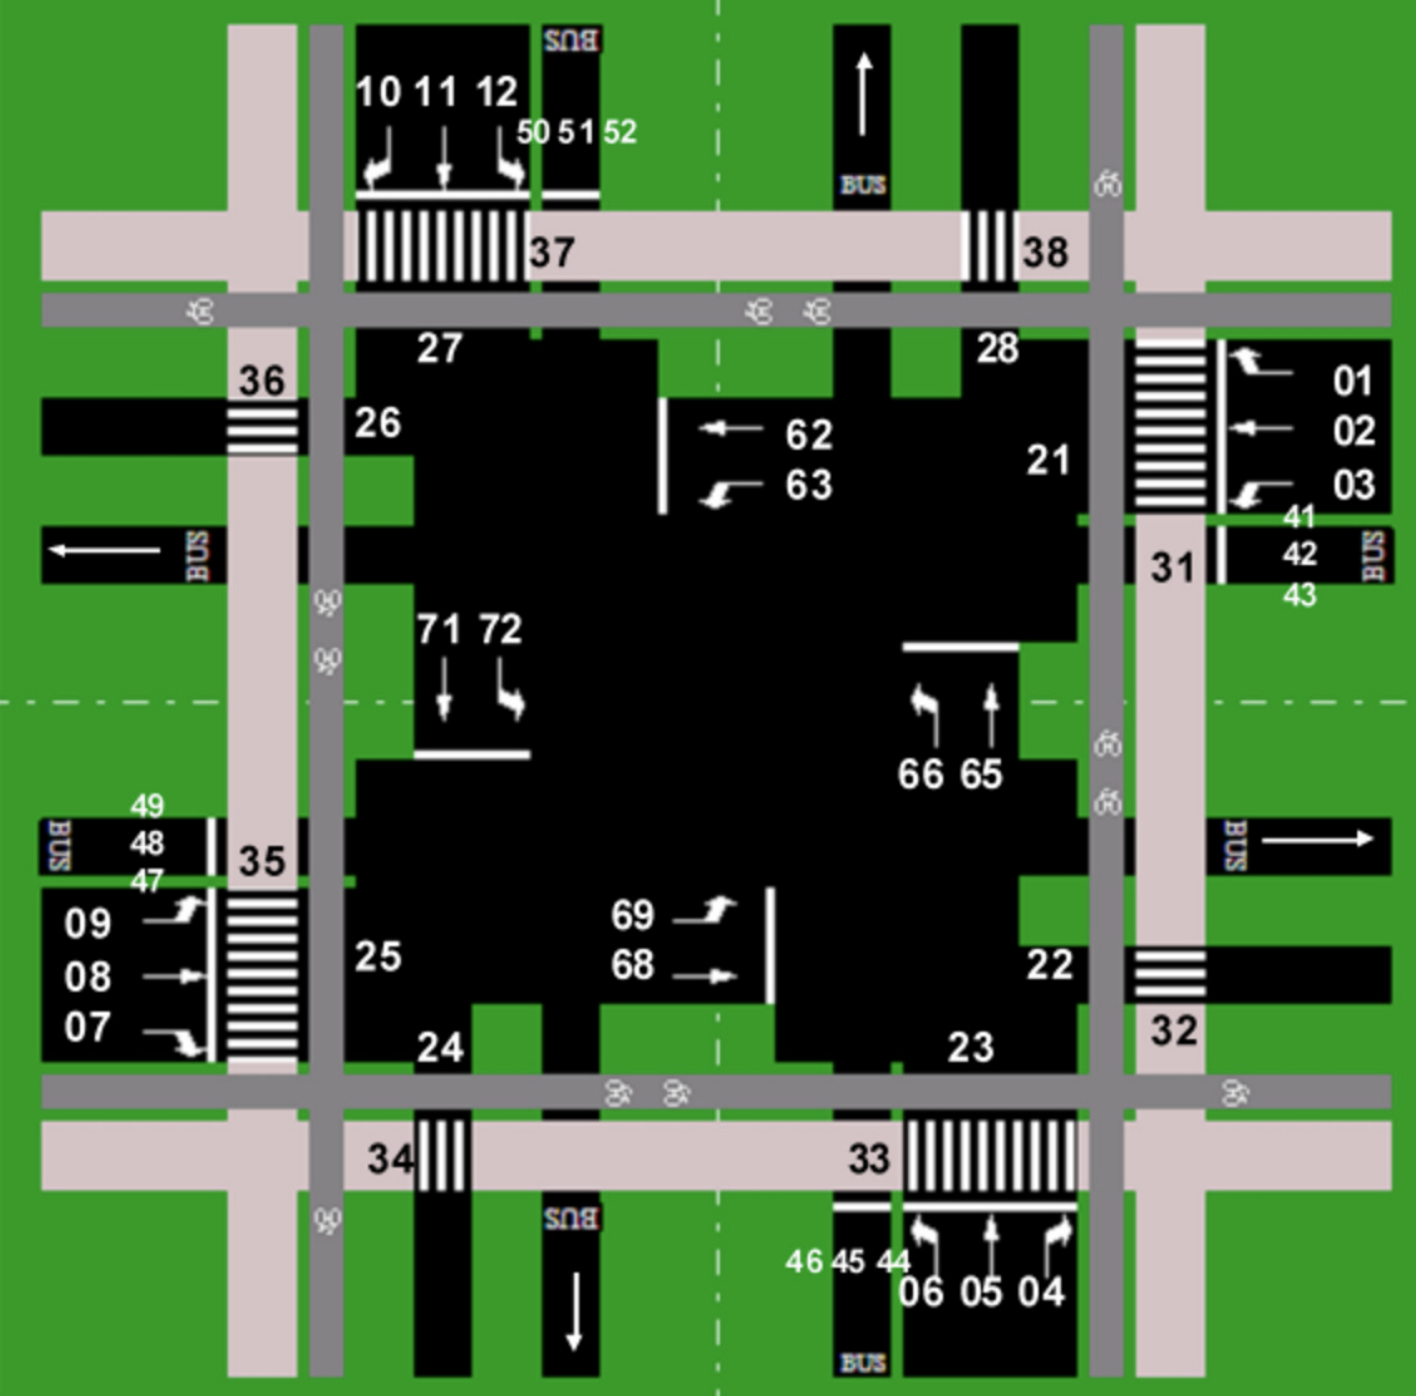
\includegraphics[width=8cm]{figures/standard.png}
    \caption{Cross Intersection layout}
    \label{fig: standard layout}
\end{figure}
  
\section{Research Questions}
To address the issue outlined in section \ref{section:Problem Statement}, this thesis presents a research objective that leads to the formulation of the research question.
\subsection{Research Objective}
The PF-SIQE, designed for real-time queue length estimation, is able to offer crucial inputs to real-time traffic signal controllers and serve as I2V (Infrastructure to Vehicle) information for connected vehicles. This could lead to improved performance at intersections, marked by reductions in traffic delays, vehicle emissions, and the incidence of vehicle crashes.
To achieve the development of the PF-SIQE, here are some specific research objectives:
\begin{enumerate}
  \item Develop a PF-SIQE architecture, along with the algorithm framework.
  \item Study various detection technologies, their outputs and the corresponding noise distribution.
  \item Building a modular mathematical model and implement in simulation.
  \item Validation of the PF-SIQE.
  \item Test the performance of the PF-SIQE to different factors such as the number of particles, penetration rate of the floating sensor, placement of loop detectors, probability of choosing stop within dilemma zone, initial condition, etc.
\end{enumerate}
\subsection{Research Contribution}
The primary contribution of this thesis is the development of a modular, scalable, flexible, and adaptable particle filter-based framework, specifically designed for real-time queue length estimation at signalized intersections. The framework is divided into three key modules: the state transition function module, the measurement function module, and the particle filter module. This modularity allows for the integration of various microscopic traffic flow models, as well as data from different detection technologies, such as loop detectors and floating car data, making the framework highly adaptable to diverse traffic conditions and data sources. 

A notable novelty of this work lies in its ability to handle uncertainties, including those with non-Gaussian noise distributions, which are common in real-world traffic scenarios. While the focus of this thesis is on signalized intersections, the framework itself has the potential to be extended to other types of intersections and roadway environments in future research. Further detailed contributions are discussed in Section \ref{LR: Conclusion}.

\subsection{Main Research Question}
How can a novel Particle Filter-based Signalized Intersection Queue Estimator (PF-SIQE) be developed for real-time queue length estimation using the particle filter algorithm, while accommodating different traffic flow models, detection technologies, and uncertainties?


\subsection{Sub Research Questions}
The sub-questions correspond directly to the research objectives:
\begin{enumerate}
  \item What is the PF-SIQE architecture along with particle filter algorithm framework? What are the modules of the framework?
  \item What are the common detection technologies? What are their output measurements and the corresponding noise characteristics?
  \item What are the mathematical descriptions of each modules in PF-SIQE framework?
  \item How to design the experiment scenarios in order to validate the PF-SIQE?
  \item What interested factors are selected to implement the sensitivity test? And why?
  \item How to abstract road layout features into the PF-SIQE architecture (future research recommendations)?
  %\item Study the estimation accuracy (also considering computational time, variance, etc.) considering (1) different penetration of probe vehicle or connected vehicle (ranging from 10\% to 90\% in increments of 10\%); (2) different numbers of loop detectors (increasing from 2 to 10); (3) the effective number of particle for various set-ups; (4) different update periods; (5) different data sources:  a. loop detector, b. probe vehicle or connected vehicle data, c. fusing loop detector and probe vehicle or connected vehicle data. (6) link length and vehicle length.
\end{enumerate}
\section{Research outline}
The research approach will result in an outline of the thesis. The list of contents at the chapter level is presented, describing the structure of the Thesis.
\begin{enumerate}
  \item Preface, Abstract, Nomenclature.
  \item Introduction, with the background and problem statement of the traffic problems, the corresponding research objectives, research questions and research contributions. 
  \item Literature review considering to:
  \begin{itemize}
      \item Comprehensive review of the real-time queue estimation methods at signalized intersection in terms of queue definition, time scale, algorithms and uncertainties.
      \item Comprehensive review of the detection technologies in terms of roadside sensors and floating sensors.
      \item Conclusion of the detailed contributions.
  \end{itemize}
  \item Methodology considering to:
  \begin{itemize}
      \item The PF-SIQE Architecture.
      \item Mathematical descriptions of the three modules: the state transition function module, the measurement function module, and the particle filter module.
  \end{itemize}
  \item Experimental simulation considering to:
  \begin{itemize}
      \item Validation of the PF-SIQE framework.
      \item Sensitivity tests to different factors such as the number of particles, penetration rate of the floating sensor, placement of loop detectors, probability of choosing stop within dilemma zone, initial condition, etc.
      \item Results and interpretation.
  \end{itemize}
  \item Discussion, conclusion, and recommendation considering to:
  \begin{itemize}
      \item Discussions on research findings, research questions, and methodology assumptions.
      \item Conclusions and implications.
      \item Recommendation for future works.
  \end{itemize}
  \item Bibliography and Appendices.
\end{enumerate}
Next chapter will present a very comprehensive literature review.
\afterpage{\blankpage}
\chapter{Literature Review}
\label{chapter:Literature Review}
Building on the general introduction provided in Chapter \ref{chapter:introduction}, this chapter serves as a critical foundation for the thesis. It reviews existing state estimation methods, and elucidates their strengths and weaknesses, to set the theoretical and conceptual groundwork for the proposed Particle Filter-Based Signalized Intersection Queue Estimator (PF-SIQE). It identifies aspects of these methodologies that align with the proposed estimator in the current thesis, highlighting where the current thesis diverges and articulates the unique contributions. This section specifies the core areas of focus, outlining the rationale behind the inclusion or exclusion of certain literature. It explains the necessity of reviewing specific works and justifies the decision to omit others, ensuring a directed and purposeful exploration of relevant research that underpins the foundation of this thesis. The insights garnered here not only inform the design principles of the PF-SIQE but also pave the way for the detailed methodological development discussed in the next chapter. 


\section{Introduction}
The objective of the PF-SIQE is to estimate the queue length as accurately as possible, even in the presence of system noise and noisy sensor measurements. Then give a well-performed estimation of the system state. In Section \ref{Queue Estimation-LR}, the literature review of existing real-time queue estimation methods not only highlights the research gap and the novelty of the proposed PF-SIQE but also identifies valuable elements from the existing literature. It gathers theories, arguments, and approaches that have proven effective, providing insights into which elements could be adapted or extended to benefit the proposed research. This comprehensive review ensures a solid theoretical foundation, allowing us to leverage previous findings while addressing the gaps identified.

The proposed PF-SIQE consists of three main modules:
\begin{itemize}
    \item The state transition function module: generates the state at $k$ based on the state at $k-1$, and gives the probability distribution function.
    \item The measurement function module: generates the measurements and gives the probability distribution function.
    \item The particle filter module.
\end{itemize}
All the modules are input as independent components within the versatile PF-SIQE framework, which allows for flexible replacement and integration.

In the state transition function module of this study, the focus is on simulating the vehicle state at time step $k$ based on its state at $k-1$. The precision of state prediction hinges on the design of the state transition function. This thesis incorporates car-following models and traffic signal status to elucidate the longitudinal movement of vehicles. The exploration of lateral movements through lane-changing models remains an avenue for future investigation. Given that car-following models serve as a flexible component within the state transition framework, implementing a literature review on different car-following models is not the primary aim of this work. Consequently, an exhaustive review of various car-following and acceleration/deceleration models is omitted from the literature review section, aligning the focus more on the application and flexibility of the model within the context of the PF-SIQE.

Given that the PF-SIQE aims to estimate the queue as accurately as possible despite the noisy system and measurements, and considering the absence of fully accurate real-life data from loop detectors, measurement generation is conducted through the measurement function module. Understanding the noise distribution in loop detector outputs is crucial. In Section \ref{detection technologies}, our examination will center on loop detectors alongside other detection methods, and study their key attributes. This includes an exploration of the types of output measurements these detectors capture, the origins of measurement noise, and the distribution of such noise. The methodology for deducing the measurement noise distribution will be outlined in Chapter \ref{chapter: Development of a Particle Filter-Based Signalized Intersection Queue Estimator (PF-SIQE)}.

In the upcoming Section \ref{Queue Estimation-LR}, Tables \ref{LR1} and \ref{LR2} present a comprehensive overview of the traditional methods of queue estimation and their evolution, categorizing them by key features such as the queue definition, time scale, data sources, estimation algorithms, and uncertainties. These categories were chosen for several reasons. First, the queue definition varies across the literature, with some studies estimating the maximum queue length within a cycle, which is crucial for assessing traffic signal performance and optimizing signal parameters, such as cycle length. Others focus on the position of the last vehicle (queue tail), and some estimate the number of vehicles. Including this category helps to understand these different approaches. Second, the time scale for queue estimation can either be cycle-by-cycle or second-by-second. Much of the previous research employed a cycle-by-cycle time scale. However, recent studies, including my thesis, focus on a higher time resolution of second-by-second estimation. This category underscores the temporal shift in research focus and its pertinence to my study. Third, including the category of data sources allows for a comparison of the various types of data and sensors utilized in previous studies, which is highly relevant to the methodology of development of the proposed PF-SIQE in Chapter \ref{chapter: Development of a Particle Filter-Based Signalized Intersection Queue Estimator (PF-SIQE)}. Fourth, estimation algorithms are a core category that provides insight into the methodologies employed in previous research and their performance. Understanding the various estimation algorithms helps to study classic algorithms, observe their evolution over time, and assess the strengths and weaknesses of each method. Lastly, how previous studies have addressed uncertainties, including system noise and measurement noise, is crucial for the robustness of estimation algorithms. This is particularly relevant to the proposed PF-SIQE, as its objective is to estimate queue length as accurately as possible, especially in the presence of system noise and noisy sensor measurements.

Given the limited number of studies specifically addressing queue estimation with the particle filter, Table \ref{LR3} compiles research that focuses on traffic state estimation and vehicle-based localization using the particle filter. The chosen categories for this table include estimated variable, time scale, level, road type, data sources, estimation algorithms, and uncertainties. The estimated variable category clarifies which specific variable within the traffic state (i.e. speed, density, or flow) is being estimated. The level category distinguishes whether the estimation is macroscopic, mesoscopic, or microscopic(i.e. vehicle-based). The road type category specifies the type of environment studied, such as signalized intersections, freeways, or urban areas. This comprehensive categorization helps to better understand the application of particle filters in related fields and their relevance to queue estimation.

Given the limited number of literature specifically addressing queue estimation with the particle filter, Table \ref{LR3} compiles studies that focus on traffic state estimation and vehicle-based localization utilizing the particle filter.

Following this broader perspective, to align with the proposed PF-SIQE and maintain focus, particular emphasis is placed on literature that addresses the following critical aspects:

\begin{itemize}
    \item The vehicle-based estimation approach, incorporates microscopic traffic flow models such as car-following models, traffic signal acceleration/deceleration models, and lane change models.
    \item High-resolution time scales on a per-second basis, aligning with the demands of real-time estimation.
    \item An exploration of the effects of system noise and measurement noise, with a focus on how previous research has managed these issues, particularly measurement noise arising from different sensors.
    \item The application of recursive Bayesian frameworks to queue estimation or traffic state estimation, with a special focus on the particle filter.
\end{itemize}
These focal points are integral to understanding the current state of queue estimation technology and formulating effective enhancements in line with the PF-SIQE.


\newgeometry{landscape, left=1cm, right=1cm, top=1.5cm, bottom=1.5cm}
\begin{landscape}
\begin{table}
\centering
\footnotesize 
\caption{Summary of Literature review on queue estimation \uppercase\expandafter{\romannumeral1}}
\label{LR1}
% 为各列分配不同的相对宽度
\begin{tabularx}{\linewidth}{@{} l 
>{\hsize=.7\hsize}X  % Literature
>{\hsize=.35\hsize}X  % Queue Definition
>{\hsize=1.2\hsize}X  % Time Scale
>{\hsize=0.8\hsize}X % Data Source
>{\hsize=1.2\hsize}X % Estimation Algorithm
>{\hsize=1\hsize}X % Uncertainties
@{}} 
\toprule
\textbf{Literature} & \textbf{Queue Definition} & \textbf{Time Scale} & \textbf{Data Source} & \textbf{Estimation Algorithm} & \textbf{Uncertainties} \\
\midrule
\textcite{sharma2007input} & maximum queue length & per cycle & roadside sensors: loop detectors & input-output model & discuss the placement of detector to enhance measurement accuracy, not intro noise \\
\textcite{liu2009real} & maximum queue length & per cycle & roadside sensors: high resolution loop detector & shockwave theory + break point & not consider detection error \\
\textcite{cheng2012exploratory} & maximum queue length & per cycle & probe trajectory & shockwave theory + critical point & not consider probe data noise \\
\textcite{cai2014shock} & maximum queue length & per cycle & Multi: probe vehicle trajectory, upstream high resolution loop detector & shockwave theory + critical point & not consider probe data noise and loop detection error \\
\textcite{lee2015real} & maximum queue length & per cycle & roadside sensors: loop detectors & input-output model + KF & count error, error caused by lane-change behaviour \\
\textcite{wang2015cycle} & maximum queue length & per cycle & Multi: location, time of probe vehicle, loop detector & shockwave theory + critical point & assume deviation of data (location) less than 3 m \\
\textcite{yin2018kalman} & maximum queue length & per cycle & mobile phone GPS: location, time step, vehicle ID & shockwave + KF & system noise $\sim$ zero-mean Gaussian distribution, measurement noise $\sim$ zero-mean Gaussian distribution \\
\textcite{an2018real} & maximum queue length & per cycle & roadside sensors: high resolution video-based detector & input-output model & assume can avoid error by choosing time period from video \\
\textcite{gao2019connected} & maximum queue length & per cycle & floating sensor: vehicle ID, location, queue time, speed of CV & shockwave + back propagation (BP) neural network & give function of back propagation of error \\
\textcite{yao2019cycle} & maximum queue length & per cycle & roadside sensors: low resolution loop detector & shockwave theory & not include effects if data quality on estimation accuracy \\
\textcite{abewickrema2023multivariate} & maximum queue length & per cycle & roadside sensors: high resolution loop detector & shockwave + KF + break point & process noise $\sim$ zero-mean multivariate normal distribution, measurement noise $\sim$ zero-mean Gaussian white noise \\
\textcite{vigos2008real} & number of vehicles & per second & roadside sensors: loop detectors & input-output model + KF & system noise $\sim$ zero-mean white Gaussian random variables, measurement $\sim$ zero-mean white Gaussian random variables \\
\textcite{vigos2010simplified} & number of vehicles & per second & roadside sensors: loop detectors & input-output model + KF & detailed analysis of system and measurement noise \\
\textcite{hao2014cycle} & number of vehicles & per cycle & mobile sensor: sample travel times & bayesian network based method & not consider any noise \\
\textcite{aljamal2020real} & number of vehicles & per second & floating sensor: location, speed of CV & AKF + AKFNN & dynamically estimate the mean and variance of state noise and measurement noise \\
\bottomrule
\end{tabularx}
\end{table}
\end{landscape}


\newpage
\begin{landscape}
\begin{table}
\centering
\footnotesize 
\caption{Summary of Literature review on queue estimation \uppercase\expandafter{\romannumeral2}}
\label{LR2}
% 为各列分配不同的相对宽度
\begin{tabularx}{\linewidth}{@{} l 
>{\hsize=0.6\hsize}X  % Literature
>{\hsize=.35\hsize}X  % Queue Definition
>{\hsize=1.2\hsize}X  % Time Scale
>{\hsize=.8\hsize}X % Data Source
>{\hsize=1.3\hsize}X % Estimation Algorithm
>{\hsize=1\hsize}X % Uncertainties
@{}} 
\toprule
\textbf{Literature} & \textbf{Queue Definition} & \textbf{Time Scale} & \textbf{Data Source} & \textbf{Estimation Algorithm} & \textbf{Uncertainties} \\
\midrule
\textcite{aljamal2020real} & number of vehicles & dynamic & floating sensor: location, speed of CV, level of market penetration (LMP) & input-output model + hydrodynamic equation + KF & no discussion of system and measurement noise \\
\textcite{wang2021kalman} & number of vehicles & per second & floating sensor: location, speed, acceleration of CV & input-output model + KF & state noise $\sim$ zero-mean multivariate normal distribution, measurement noise $\sim$ zero-mean Gaussian white noise \\
\textcite{comert2021queue} & number of vehicles & per cycle & floating sensor: location, time of CV, whether there is a follower & analytical probabilistic model & assume lane level accuracy for CV locations \\
\textcite{anusha2022dynamical} & number of vehicles & per cycle & roadside sensors: synchronized video cameras located at the entry and exit of intersection & input-output model + KF & model the mean and variance of process and measurement noise for different scenarios, including lane change \\
\textcite{ferencz2023road} & Queue length & per cycle & Simulation data: speed, distance & Shockwave + AI based KF & Process noise $\sim$ zero-mean multivariate normal distribution, Measurement noise $\sim$ zero-mean Gaussian white noise \\
\textcite{ban2011real} & Queue length & per cycle & Mobile sensor: sample travel times & Shockwave theory & No consideration of noise \\
\textcite{cheng2011cycle} & Queue length & per cycle & Sampled floating sensor: location, speed, time of probe vehicle & Shockwave theory + critical point & Location, speed projection error \\
\textcite{comert2013simple} & Queue length & per cycle & Floating sensor: location, time of probe vehicle & Analytical probabilistic model & No consideration of probe data noise \\
\textcite{ramezani2015queue} & Queue length & per cycle & Floating sensor: location, speed of probe vehicle & Shockwave theory & Measurement noise $\sim$ zero-mean Gaussian distribution \\
\textcite{yang2018queue} & Queue length & per cycle & Floating sensor: CV's trajectory points & Shockwave + convex optimization + critical point & Claims to handle measurement noise, no noise distribution \\
\textcite{wang2020queue} & Queue length & per cycle & Floating sensor: location, speed of probe vehicle; onset of red & Shockwave + integer programming & No consideration of probe data noise \\
\textcite{tan2020fuzing} & Queue length & per cycle & Multi: location, time of probe vehicle; license plate recognition: license plate number, time, vehicle type & Bayesian theory & Quality of LPR and probe data not considered \\
\textcite{hu2022high} & Queue tail & per second & Floating sensor: location \& speed of CV, spacings \& speed of predecessor and follower & Shockwave + EKF & Measurement noise $\sim$ zero-mean Gaussian white noise \\
\bottomrule
\end{tabularx}
\end{table}
\end{landscape}


\begin{landscape}
\begin{table}
\centering
\footnotesize
\caption{Summary of Literature Review on Traffic State Estimation with Particle filter \uppercase\expandafter{\romannumeral3}}
\label{LR3}
\begin{tabularx}{\linewidth}{@{} 
>{\hsize=0.7\hsize}X  % Literature
>{\hsize=0.6\hsize}X  % Estimated Variable
>{\hsize=0.45\hsize}X  % Time Scale
>{\hsize=0.45\hsize}X  % Level
>{\hsize=0.5\hsize}X  % Road Type
>{\hsize=1\hsize}X    % Data Source
>{\hsize=1.2\hsize}X  % Estimation Algorithm
>{\hsize=1.5\hsize}X    % Uncertainties
@{}} 
\toprule
\textbf{Literature} & \textbf{Estimated Variable} & \textbf{Time Scale} & \textbf{Level} & \textbf{Road Type} & \textbf{Data Source} & \textbf{Estimation Algorithm} & \textbf{Uncertainties} \\
\midrule
\textcite{chen2011real} & speed profile & 5 min & macroscopic & freeway & roadside sensors: speed from loop detector per min & Van Aerde flow continuity model + PF & process, measurement noise, no distribution given \\
\textcite{aljamal2020real} & number of vehicles & per second & macroscopic & signalized intersection & floating sensor: location, speed of CV, LMP & input-output model + hydrodynamic equation + PF & process, measurement noise distribution is not given \\
\textcite{peker2011particle} & localization & per second & vehicle-based & urban & GPS and odometer of vehicle; digital map & PF with map topology & state faults, measurement error distribution is not given \\
\textcite{mihaylova2007freeway} & density, speed & per second & macroscopic & freeway & roadside sensors at segments boundaries & a compositional stochastic model based on cell-transimission model + PF & missed count and false detection ~ Poisson random variables, speed noise ~ Gaussian distribution \\
\textcite{fang2019road} & center location & per second & vehicle-based & urban & floating sensor: on-vehicle visual detection: center location & part-based PF & a small Gaussian noise is added during importance sampling \\
\textcite{mihaylova2012parallelized} & flow, density, speed & 10-second & macroscopic & freeway & roadside sensors at segments boundaries & parallelized PF + parallelized Gaussian sum PF & state and measurement noise ~ Gaussian \\
\textcite{xie2018generic} & vehicle trajectories, flow, density & per second & macroscopic, vehicle-based & signalized intersection & multi: loops, traffic control data, sparse travel time & a generic data assimilation framework, IDM + PF & count error ~ discrete probability distribution, system noise distribution is not given \\
\bottomrule
\end{tabularx}
\end{table}
\end{landscape}
\restoregeometry


\section{Real-time Queue Estimation at Signalized Intersections}\label{Queue Estimation-LR}
Queue estimation is an integral component of traffic state estimation, which itself is influenced by vehicle localization. Although there is limited literature specifically focused on real-time queue estimation using vehicle localization, the current thesis aims to tackle this issue. Queue estimation has been extensively researched for both freeways and signalized intersections. To emphasize the research gap between previous studies and this thesis, this Section narrows the scope to focus on queue estimation at signalized intersections.

After a comprehensive literature review in this area, the summary of the literature on real-time signalized intersection queue estimation is shown in Tables \ref{LR1} and \ref{LR2}. It is revealed that research mainly concentrates on several critical aspects: 
\begin{itemize}
    \item the queue definition, i.e. the target output, and time scale for different purposes;
    \item the methodologies and algorithms;
    \item the detection technology, data source, and uncertainties.
\end{itemize}
Section \ref{Queue Estimation-LR} will be organized according to these aspects. Furthermore, to align with the objective of using the particle filter approach in this thesis, Table \ref{LR3} presents current studies that utilize the particle filter for vehicle localization and traffic state estimation. Although few studies focus on queue estimation using the particle filter, the existing works are still informative. Additionally, other relevant aspects, such as lane change behaviors, signal control types, and arrival patterns, will be discussed in the Summary Section \ref{queue estimation summary}.



\subsection{Queue Definition and Time Scale}

The queue definition and the selection of a time scale vary according to different study purposes. In terms of the macroscopic queue estimation for traffic management, estimating the maximum queue length, which denotes the maximum value of queue lengths within a cycle is a good choice (\textcite{sharma2007input}, \textcite{liu2009real}, \textcite{cheng2012exploratory}, \textcite{cai2014shock}, \textcite{lee2015real}, \textcite{wang2015cycle}, \textcite{yin2018kalman}, \textcite{an2018real}, \textcite{gao2019connected}, \textcite{yao2019cycle}, \textcite{abewickrema2023multivariate}). Queue accumulation starts at the onset of the red interval and disperses at the beginning of the green phase; however, it is possible that during the green phase, newly arriving vehicles also begin to queue at the end of the queue. Consequently, the cycle-based measurement of queue lengths is categorized into two types: one that exclusively records vehicles arriving during the red signal period, and another that tracks vehicles arriving throughout both the red and green signal periods. \textcite{sharma2007input} define the counting period for each cycle as ending after the red signal plus the start-up lost time. They also establish a queue failure flag when the maximum queue length for a cycle meets or exceeds the storage capacity of that lane. \textcite{liu2009real} consider the maximum queue length during both the red and green period.

The rear/back of the queue (\textcite{hu2022high}), often referred to as queue tail location, indicates the position of the last vehicle in the queue at a certain time step. This information is crucial for determining the placement of point detectors (such as loop detectors and video cameras) and for designing the length of road segments between intersections in road network design. 

Queue length, commonly defined as the distance from the rear of the queue to the stop line 
(\textcite{ban2011real}, \textcite{cheng2011cycle}, \textcite{comert2013simple}, \textcite{ramezani2015queue}, \textcite{yang2018queue}, \textcite{wang2020queue}, \textcite{tan2020fuzing}, \textcite{ferencz2023road}) or the number of nearly stationary vehicles (\textcite{vigos2008real}, \textcite{vigos2010simplified}, \textcite{hao2014cycle}, \textcite{aljamal2020real}, \textcite{wang2021kalman}, \textcite{comert2021queue}, \textcite{anusha2022dynamical}, \textcite{ferencz2023road}) at a certain time step, is also widely utilized for monitoring the traffic flow. 

In the context of real-time queue estimation at signalized intersections, research typically focuses on evaluating signal performance, optimizing the signal timings, and synchronizing signals between upstream and downstream intersections, making cycle-based estimations highly valuable. Although most studies operate on a cycle-by-cycle time scale, \textcite{vigos2008real}, \textcite{vigos2010simplified}, \textcite{aljamal2020real}, \textcite{wang2021kalman}, and \textcite{hu2022high} have employed more granular second-by-second analyses. This finer time resolution is crucial for vehicle-based estimation and vehicle localization, pivotal technologies in connected vehicles that offer significant potential for application in intelligent transportation systems. Therefore, exploring queue estimation algorithms that utilize a second-by-second time scale is of paramount importance, an objective this paper directly addresses.

\subsection{Methodologies and Algorithms}\label{LR: Methodologies and Algorithms}
In traffic queue estimation, extensive research has been conducted utilizing theoretical frameworks such as shockwave theory and the input-output model, commonly referred to as the flow continuity equation. \textcite{ramezani2015queue} propose a method to estimate queue profiles as traffic shockwave polygons in the time-space plane, capturing the spatiotemporal formation and dissipation of queues. This method combines the collective effect of dispersed probe vehicle data with traffic flow shockwave analysis and data mining techniques. The queue profile estimation relies on position and velocity data from probe vehicles, while explicit information about signal settings and arrival distribution is essential. Numerical results from simulation experiments and tests on NGSIM field data with varying penetration rates and sampling intervals show that the proposed method performs promisingly and robustly compared to a uniform arrival queue estimation procedure. Seminal works based on shockwave theory include studies by \textcite{liu2009real}, \textcite{cheng2012exploratory}, \textcite{cai2014shock}, \textcite{wang2015cycle}, \textcite{gao2019connected}, \textcite{yao2019cycle}, \textcite{ban2011real}, \textcite{cheng2011cycle}, , and \textcite{wang2020queue}. Another common method for estimating vehicle count is the input-output approach, also known as the traffic flow continuity equation. This method involves using two traffic counting stations, one located at the entrance and the other at the end of the roadway link. Studies by \textcite{sharma2007input} and \textcite{an2018real} are also based on the input-output approach.

 \textcite{vigos2008real} explains that while it is theoretically feasible to use the measurements of inflow and outflow to estimate vehicle counts \(N(k)\), the number of vehicles between two measurement points, this approach inherently results in the accumulation of measurement noise, which subsequently degrades the accuracy of these estimates over time. To mitigate this issue, \textcite{lee2015real}, \textcite{vigos2008real}, \textcite{vigos2010simplified}, \textcite{aljamal2020real}, \textcite{wang2021kalman} and \textcite{anusha2022dynamical} advocates using an input-output model combined with bayesian filtering techniques, such as the Kalman Filter (KF). Similarly, there are some studies combining shockwave theory and filter techniques, see \textcite{yin2018kalman}, \textcite{abewickrema2023multivariate}, \textcite{ferencz2023road}, \textcite{hu2022high}. 

\textcite{hu2022high} develop a high-resolution approach for estimating queue profiles at urban intersections, utilizing an Extended Kalman Filter (EKF) based on shockwave theory. The approach assumes measurement noise follows a zero-mean Gaussian white noise distribution. The prediction of this model is powered by a machine learning-based dynamic shockwave propagation model that learns from historical data of connected vehicles (CVs). Correction of the model is achieved through data fusion-based shockwave sensing. This prediction-correction structure parallels the methodology in the current thesis, which, instead of utilizing EKF, employs a particle filter (PF) for estimating queue lengths and can counter any non-Gaussian noise in the system and measurement.

Specifically, the investigations of \textcite{wang2015cycle}, \textcite{cheng2012exploratory}, \textcite{cai2014shock}, and \textcite{cheng2011cycle} highlight the utilization of probe trajectory data to pinpoint the critical point within traffic flows. Critical points (CP) are defined as the data points representing the changes in vehicle dynamics and can be extracted using different algorithms. For instance, \textcite{cheng2012exploratory} utilizes the approach where the trajectory between two critical points (CPs) is clearly defined and falls into one of two basic movements: (a) uniform motion, which includes stopping as a special case, and (b) uniformly accelerated motion, which also encompasses deceleration. Thus, a trajectory can be segmented into various regimes with CPs serving as the boundaries, where each regime corresponds to one of these two fundamental movements.

\textcite{gao2019connected} introduces a queue length sensing model that leverages V2X technology, incorporating sub-models based on shockwave sensing and a back propagation (BP) neural network. The model analyzes state information from connected vehicles to understand queue formation and predict lengths by calculating shockwave velocities and using a BP neural network trained on historical data. These sub-models are then integrated using variable weights to determine real-time maximum queue lengths at intersections.

\textcite{wang2020queue} develop an integer programming model featuring a set of constraints designed to estimate the queue profile, adhering to the spatiotemporal propagation of shockwaves. The novelty of the approach lies in its ability to detect queue profiles of any shape, contrasting with other studies that typically use triangles or polygons for approximation.

Queue estimation also utilizes analytical and probabilistic models based on the Bayesian network, as demonstrated in studies by \textcite{hao2014cycle}, \textcite{comert2021queue}, \textcite{comert2013simple}, and \textcite{tan2020fuzing}.  Particularly, recursive Bayesian frameworks such as the Kalman filter and its variations (EKF, AKF, UKF) and particle filter, consisting of a state update process (prediction) and measurement update process (correction). The sequence of these processes differentiates data estimation from prediction tasks. In traffic state estimation, once current measured data are available, they are used to refine the estimated values. Due to some ambiguity surrounding the terms estimation and prediction in the literature, this thesis defines estimation as referring to the current state and prediction as referring to future states. Conversely, predictions are generated using estimated values in the time update equation (\textcite{chen2011real}). Moreover, this recursive approach ensures that traffic state data are efficiently computed using only the data from previous states, rather than the entire historical dataset (\textcite{ristic2003beyond}).

\textcite{aljamal2020real} conducted extensive research on real-time traffic stream density estimation at signalized intersections, focusing on the number of vehicles, time scales, and addressing uncertainties through the evolution of estimation algorithms. His work is pivotal in understanding the effectiveness of various methodologies, particularly the Kalman filter (KF), adaptive Kalman filter (AKF), and particle filter (PF). Aljamal demonstrated that the linear Kalman filter approach, while effective, showed limitations under certain conditions, such as low market penetration (LMP) of connected vehicles (CVs) and the presence of trucks. To address these limitations, he developed an adaptive Kalman filter (AKF) that dynamically estimates system and measurement noise, significantly improving estimation accuracy. In advancing the estimation algorithms, Aljamal also introduced a nonlinear Particle Filter (PF) approach. He found that while the PF's accuracy improves with an increased number of particles and higher CV penetration, it is highly sensitive to initial conditions. Conversely, the KF approach was less sensitive and provided more consistent performance, leading Aljamal to conclude that the KF generally outperformed the PF for macroscopic traffic density estimation. However, there is a research gap that the proposed PF-SIQE aims to address. Unlike Aljamal’s macroscopic focus on the number of vehicles, the PF-SIQE is designed for vehicle-based localization, estimating the location of all vehicles within the intersection and their dynamic movements over time. This vehicle-based approach leverages the scalability, modularity, and suitability of the particle filter for addressing the nonlinear nature of vehicular dynamics. Previous studies by Peker et al. (2011) and Fang et al. (2019) have successfully utilized vehicle-based particle filter frameworks for localization issues, indicating its common application in such contexts. Thus, despite Aljamal's findings favoring the KF for vehicle count estimation, the PF is expected to perform better in vehicle-based localization due to its robustness in handling nonlinearities in vehicular dynamics.

The Kalman filter approach, commonly used in handling uncertainties, assumes that both system noise and measurement noise follow a Gaussian distribution. This assumption implies a predictable, regular pattern of variability that is statistically manageable. However, this assumption may not hold at signalized intersections where driver behavior becomes more complex due to the yellow light. At this phase, drivers enter what is known as the decision-making dilemma zone, where they must quickly decide whether to stop or proceed through the intersection. This decision is influenced by several factors including speed, distance to the intersection, and personal risk assessment, which introduces a non-linear and often non-Gaussian behavior in driver responses (\textcite{gates2007analysis}). The unpredictability introduced by the dilemma zone conflicts with the Gaussian noise assumptions of the Kalman filter, potentially complicating the accuracy of estimations at these critical traffic points. \textcite{helbing2001traffic} found that vehicular traffic exhibits highly nonlinear behavior, characterized by complex interactions among vehicles. Therefore, the vehicle dynamic may not be adequately captured by a Gaussian distribution. Moreover, the assumption of Gaussian distribution may fail to fully address various types of detection noise such as the miss count or double count errors commonly found with loop detectors. The issue could be better modeled using a discrete probability distribution, which represents another significant contribution of this thesis in Chapter \ref{chapter: Development of a Particle Filter-Based Signalized Intersection Queue Estimator (PF-SIQE)}.

Although research utilizing particle filters for queue estimation is scarce, their application in traffic state estimation has been explored. 
In both single-lane and multi-lane scenarios, where traffic conditions are stationary and homogeneous, the number of vehicles can be calculated by multiplying the traffic density by the road length. Various traffic models (such as Greenshields-based CTM-V model, Van Aerde flow continuity model) and recursive Bayesian filtering techniques (such as Ensemble Kalman filter and Particle filter) have been employed to estimate traffic state variables in recent years, see \textcite{wang2005real}, \textcite{mihaylova2007freeway}, \textcite{sau2007particle}, \textcite{work2008ensemble}, \textcite{cheng2006traffic}, and \textcite{chen2011real}. Notably, the particle filter has been identified as particularly effective due to its capability to handle nonlinear updates of traffic variables (\textcite{sau2007particle}).

\textcite{peker2011particle} and \textcite{fang2019road} utilize a vehicle-based particle filter framework to address localization issues, a topic also of interest in this thesis. \textcite{peker2011particle} present a novel algorithm for vehicle localization and map-matching using a particle filter aided by digital maps. Their algorithm enhances the likelihood function during the weight calculation step of the particle filter by incorporating the probability of a vehicle being in a certain area of the digital map based on its speed, combined with routing information. Similarly, \textcite{fang2019road} propose a part-based particle filter for on-road vehicle tracking. This model integrates a part-based strategy with a particle filter by introducing a hidden state that represents the vehicle's center position, allowing for efficient collective updating of particles. However, the proposed PF-SIQE in this thesis addresses a different set of challenges and objectives. Unlike \textcite{peker2011particle} and \textcite{fang2019road}, which focus primarily on vehicle localization and tracking, the PF-SIQE aims to localize the positions of all vehicles within a road segment at an intersection. Our method leverages car-following behavior and responses to traffic signals to estimate queue lengths and provide comprehensive queue information. Additionally, the PF-SIQE focuses on capturing the dynamics of queues, detailing how they evolve over time. This approach is designed to address the specific needs of traffic management at signalized intersections, offering insights into queue formation and dissipation that are crucial for optimizing traffic flow and reducing delays.

Particle filters have been developed for traffic state estimation across both freeways and signalized arterials by various researchers. \textcite{mihaylova2007freeway} applied particle filters to estimate density and speed on freeways using data solely from roadside sensors located at road segment boundaries, highlighting the framework's scalability, modularity, and suitability for addressing the nonlinear nature of vehicular traffic. They modeled the count of missed count and false detections as Poisson random variables and assumed Gaussian distribution for speed noise. Additionally, \textcite{mihaylova2012parallelized} introduced innovative parallelized particle filter and Gaussian sum particle filter methods for enhancing traffic state estimation. With the inspiration from \textcite{mihaylova2007freeway}, particle filter framework is used in this thesis. \textcite{chen2011real} explored the effectiveness of the particle filter framework with the Van Aerde flow continuity model, demonstrating speed estimation on freeways compared to the Extended Kalman Filter (EKF). Meanwhile, \textcite{aljamal2020real} employed a particle filter based on the input-output model and hydrodynamic equations to estimate vehicle numbers at signalized intersections.  

A very interesting study by \textcite{xie2018generic} presents a generic data assimilation framework for estimating vehicle trajectories and traffic state variables. This framework is both macroscopic and vehicle-based, incorporating the Intelligent Driver Model (IDM), a microscopic traffic flow model, into the state update process. This process is versatile and highly modular, allowing for the integration or replacement with other microscopic traffic models, such as those for lane changing. This demonstrates the adaptability of the particle filter. In this thesis, IDM is also implemented as part of the state transition function within the particle filter framework. The primary distinction between \textcite{xie2018generic} and this thesis lies in the focus of the proposed PF-SIQE on modeling the decision probability of drivers' responses to yellow lights at signalized intersections, particularly within dilemma zones, and the associated acceleration and deceleration behaviors. Additionally, the PF-SIQE considers a broader range of detector types and locations (of roadside sensors).  The thesis believes that such complex, decision-making processes are well-suited to the particle filter's capabilities in handling nonlinearity.


\subsection{Uncertainties}
In Section \ref{LR: Methodologies and Algorithms}, it is mentioned that the accumulation of measurement noise in the state equation is unignorable. It is indispensable to study various detection technologies, analyze the corresponding measurement noise distribution from the data source, and devise strategies to deal with this noise to improve the estimation accuracy. In this section, the thesis generally discusses the prevalent uncertainties encountered in queue estimation. Further details about various detection technologies will be elaborated in Section \ref{detection technologies}.

Generally, two primary types of noise must be addressed: system noise and measurement noise. An example of the difference in drivers is the throttle response of a vehicle driving on a road is influenced by inherent characteristics of the vehicle itself, which include certain biases. Additionally, as the vehicle travels, factors such as wind resistance, road curvature, and gradients can cause the actual speed or acceleration to deviate from theoretical predictions.
\textcite{ajitha2015real} highlighted the significance of understanding the characteristics of system noise to manage it effectively and enhance model performance.  In real-world applications, estimating the statistical characteristics of system noise, namely mean and variance can be challenging. To address this issue, \textcite{chu2005adaptive} have developed the adaptive Kalman filter (AKF) for estimating freeway travel time using data from both loop detectors and connected vehicles (CVs). They utilized the method for estimating noise statistical parameters originally proposed by \textcite{myers1976adaptive}. However, they still assume a Gaussian distribution for the system noise, which may not fully capture the randomness and complexity in the modeling process. In this thesis, the approach to system noise is not confined to a Gaussian distribution but is open to any formulation of noise, making it more closely aligned with real-world conditions. This flexibility represents the significant contribution of the thesis.

Measurement noise typically arises from various detection technologies involving commonly used sensors, which include both roadside sensors and floating sensors. Roadside sensors frequently employed in queue estimation encompass loop detectors, video-based detectors, license plate recognition systems, and push buttons producing information on occupancy, speed, counts, traffic flow images, license plate numbers, and vehicle types. Similarly, measurements from detection sensors are often subject to various errors. For instance, errors such as missed or double counts are common with loop detectors, \textcite{mihaylova2007freeway} introduced the number of vehicles that a detector missed and the number of false detections in freeway as independent Poisson random variables, yet there is scant literature offering solutions to these problems in signalized intersections. Another significant challenge with roadside sensors is their placement. In congested conditions, queues may extend beyond the location of the roadside sensors, making it difficult to estimate the extent of queues that are not directly observable. \textcite{sharma2007input} briefly discusses the placement of roadside sensors to improve measurement accuracy. While the distribution of measurement noise is not given, it still inspires the consideration that future research could explore how different placements of roadside sensors might impact data quality. Building on this, the proposed PF-SIQE incorporates the placement of roadside sensors by adding a variable $d_\text{detector}$ in Chapter \ref{chapter: Development of a Particle Filter-Based Signalized Intersection Queue Estimator (PF-SIQE)}, which indicates the placement of the detector, thereby acknowledging the potential impact of sensor location on the estimation. \textcite{anusha2022dynamical} developed a Kalman filter approach based on the input-output model to estimate both queue within advance detector (QWAD), and queue beyond advance detector (QBAD), which address the exceeding issue.

Research papers often use two loop detectors, positioned at the entry and exit of a traffic link, to measure inflow and outflow, subsequently applying the flow continuity equation to calculate the number of vehicles. However, the literature, including \textcite{anand2014data} and \textcite{vigos2008real}, notes that noise in the data from loop detectors can lead to significant estimation errors. To mitigate this noise, \textcite{vigos2008real} suggests incorporating an additional loop detector midway along the link. Yet, the implementation of this model is costly, requiring at least three loop detectors. In practice, many loop detectors have been in place for years and their placement is often not optimal. Therefore, there is a need to explore methods and algorithms that can address this noise without necessitating the reinstallation or addition of more roadside sensors, as a measure to control costs.

On the other hand, common floating sensors comprise GPS-equipped probe vehicles, mobile phone GPS, connected vehicles, mobile sensors, and on-vehicle sensors producing information on vehicle ID, location, time, speed, acceleration, whether there is a follower, spacing from the predecessor and follower, the speed of predecessor and follower, and sample travel time. For floating data, the level of market penetration (LMP) is recognized as a critical area of research and might determine the extent to which estimation results are affected by measurement noise. \textcite{hu2022high} conclude that connected vehicles (CVs) with low market penetration rates (MPRs) provide limited real-time information, whereas the shockwave propagation model, derived from historical data, is less susceptible to Gaussian white noise. Conversely, when MPRs are relatively high, the impact of noise becomes more pronounced.

\textcite{lee2015real} develop a Kalman filter approach based on the input-output model to counter the detection error and the error caused by lane change behavior. Similarly, \textcite{anusha2022dynamical} develop a Kalman filter approach based on the input-output model, modeling the mean and variance of process and measurement noise for various scenarios, including lane changes. Both \textcite{yin2018kalman}, and \textcite{vigos2008real} utilized a Kalman filter approach, incorporating process and measurement noise as zero-mean Gaussian distributions. Meanwhile, \textcite{abewickrema2023multivariate} and \textcite{wang2021kalman} employed a Kalman filter approach where the process noise is modeled as a zero-mean multivariate normal distribution, with measurement noise as zero-mean Gaussian white noise.  \textcite{vigos2010simplified} presented a detailed analysis of process and measurement noise in their Kalman filter approach based on the input-output model. \textcite{aljamal2020real} introduced a Neural Kalman filter (AKFNN) approach that combines an adaptive Kalman filter (AKF) with an artificial neural network (ANN). This approach uses the ANN to estimate the mean and variance of state noise and measurement noise at each time step. \textcite{ferencz2023road} developed an AI-based Kalman filter approach informed by shockwave theory, where both process and measurement noise are treated as zero-mean multivariate and Gaussian white noise, respectively.

Research employing particle filters, such as those by \textcite{mihaylova2007freeway} and \textcite{xie2018generic}, focuses on addressing detection errors from roadside sensors, including missed counts, over-counts, and false detections. \textcite{mihaylova2007freeway} modeled both missed and false detections as Poisson random variables. On the other hand, \textcite{xie2018generic} developed data error models to address vehicle accumulation errors as well as missed and over-count errors. To study the probability distribution of vehicle accumulation errors, they derived discrete probability distributions from various probable sets of vehicle trajectories based on the data. Additionally, missed and over-count errors were specifically characterized by parameters of detection accuracy and the occurrence rate of over-counts. This approach is consistent with the methodology of the current thesis, which involves extracting a discrete probability distribution from the product requirement provided by loop detector manufacturers. This extraction technique complements the detection accuracy parameters outlined by \textcite{xie2018generic}, reinforcing the thesis's framework. 

Moreover, since particle filters can effectively filter a wide range of non-Gaussian noises, the focus shifts to accurately obtaining the noise distributions for system and measurement noise as they occur in real-world settings. It is foreseeable that if the thesis can more precisely establish distributions for various types of noise encountered in real life, the estimator proposed in this thesis will yield results that are much closer to real-world outcomes.

\subsection{Summary}\label{queue estimation summary}
Most previous studies on queue estimation have taken a macroscopic approach based on shockwave theory or input-output model, often making assumptions about parameters that inherently involve microscopic vehicle dynamics, such as assuming Poisson arrival patterns for vehicle arrivals. When addressing system noise and measurement noise, many studies rely on a recursive Bayesian framework, with the Kalman filter and its variants (Extended Kalman Filter, Ensemble Kalman Filter, Unscented Kalman Filter, and Adaptive Kalman Filter) being particularly popular. While the Kalman filter (KF) is effective in tracking the mean and variance of the process state probability distribution function (pdf), it is important to note that it assumes the shape of the pdf remains Gaussian. If the pdf has a non-Gaussian shape, the KF can still correctly predict the mean and variance, but it may not capture the changing shape of the pdf accurately over time. This can be a limitation when dealing with complex, non-Gaussian noise distributions, such as those arising from nonlinear vehicular dynamics.

To encounter the challenges of nonlinearity, the particle filter (PF) has gained increasing attention. The particle filter framework offers several advantages for addressing traffic state estimation problems, including:
\begin{enumerate}
    \item The ability to handle the inherent nonlinearity of vehicular traffic dynamics.
    \item Scalability and modularity, which allow for the integration of various microscopic traffic models that more accurately reflect vehicle dynamics.
\end{enumerate}

In this current thesis, the particle filter framework allows for more flexibility in assumptions and constraints. For instance, it is unnecessary to set signal control timings to fixed or actuated controls as a baseline, assume specific vehicle arrival patterns, or require optimal placement of loop detectors. 

Other fascinating aspects of capturing vehicle dynamics include how vehicles react to signal timings, particularly the yellow light, the lane-changing behavior as they approach an intersection, and the arrival patterns at signalized intersections, with a special focus on platoon-correlated arrivals. These factors are critical in understanding and modeling the complex interactions that occur at intersections, which can significantly influence traffic flow and queue dynamics. One of the principal contributions of this thesis is the development of a decision-making model that simulates how drivers respond to traffic signals, particularly during the yellow light within the dilemma zone. This model is integrated into the state transition function module of the particle filter framework. The probability of the go or stop decision is modeled to reveal the randomness in vehicular dynamics. The state transition function is instrumental in generating ground truth simulated data. Upon receiving measurements from the measurement function, the proposed PF-SIQE provides estimations of the states (including location, speed, and acceleration) of all vehicles at each time step within the study area. Each particle carries the estimations of all the states for all vehicles at the current time step, with the assumption that these state estimations are known to each vehicle, thereby enhancing a vehicle's perception of its surrounding traffic environment. This approach not only improves the accuracy of the traffic model but also significantly enhances the real-time operational intelligence of the system.

Studying the lateral vehicular dynamics at multi-lane signalized intersections, such as predicting lane change behavior for both the vehicle itself and surrounding vehicles, presents a fascinating area of research.  This thesis lays a solid foundation for future work on lateral vehicle motions, offering a robust starting point for developing more nuanced models that can accurately capture the complexities of lane changes at intersections. Considering the platoon arrival pattern is crucial due to the widespread implementation of actuated control timing at traffic signals. One of the guiding principles of such control is to clear all waiting vehicles at an intersection by adjusting the green time. This approach leads to a phenomenon where vehicles automatically form a platoon and progress from the downstream to the upstream intersection. The interactions within these platoons, where vehicles can communicate with each other, present an interesting area for future study. It is anticipated that incorporating this factor into the estimation scheme will yield improved results, as understanding and modeling these vehicle-to-vehicle communications can enhance the accuracy and efficiency of traffic management systems.

\section{Detection Technologies}\label{detection technologies}

Given the effectiveness of the particle filter integrated with the Intelligent Driver Model (IDM) in managing nonlinear uncertainties in both system and measurement, as demonstrated by \textcite{xie2018generic}, a critical focus now shifts to studying and constructing the measurement noise distribution. Data is not only invaluable in the estimation process, such as when constructing the state transition function, but also essential for validating and calibrating the model. Therefore, this section will extensively explore the common detection technologies used in queue estimation, providing a detailed examination of how these methods contribute to the accuracy and reliability of traffic models.

Detection technologies can be categorized based on the data type of sources into Eulerian sensors, Lagrangian sensors, and third-party vendors (\textcite{klein2024roadside}). Additionally, Eulerian sensors can be categorized based on installation methods into intrusive and nonintrusive sensors, and based on the way they transmit and receive energy into passive and active sensors. While some sensors can be considered as point-based roadway sensors, others, such as long queue sensors (e.g., loop detectors), cannot be viewed as a single point. Table \ref{DT1} and \ref{DT2} shows the categorization of the detection technologies. 

\textcite{klein2024roadside} summarize the collection of traffic data has significantly advanced with the inclusion of a diverse range of sensors, such as inductive loop detectors (ILD), magnetometer sensors, magnetic sensors, video detection systems (VDS) using image processing with visible spectrum and infrared cameras, microwave radar sensors (including presence detecting microwave radar sensors and Doppler microwave sensors), passive infrared (PIR) sensors, LiDAR sensors, acoustic sensors, and ultrasonic sensors. These can be regarded as Eulerian sensors. 

The Lagrangian sensors, which move with the traffic flow (\textcite{bayen2010mobile}), includes probe vehicles (\textcite{turner1998travel}), or floating cars, which can provide traffic management centers with emissions information along with standard traffic flow parameters linked to a vehicle via GPS data (\textcite{pack2021use}) or other global navigation satellite systems’ location devices. Additional methods include cell phone tracking through media access control address readers, automatic license plate readers, toll tag (radio-frequency identification transponder) readers, taxi fleet sources, and trucking industry transponders (\textcite{singer2013travel}).

\textcite{klein2024roadside} mention that third-party data sources include HERE, INRIX, Miovision, StreetLight, TomTom, Waze, and Wejo (\textcite{coifman2013assessing}; \textcite{mccracken2016assessment}; \textcite{tsapakis2021independent}) which provide measurements of speed, travel time, flow rate, incident reporting, analytics, and OD programs.

Different sensors have vastly different application scenarios. For example, magnetometer sensors can be installed on bridge decks where inductive loop detectors (ILDs) may be affected by the steel support structure or simply cannot be installed due to other constraints (\textcite{klein2024roadside}). However, in this section, the distinction between applications and scenarios is minimized because the thesis focuses primarily on detection technologies that can be used at signalized intersections.

To ensure the literature review aligns with the objectives of the thesis, it is crucial to investigate several key aspects:
\begin{itemize}
    \item The measurement output of each sensor type;
    \item The noise distribution associated with these measurements;
    \item The advantages and disadvantages of each sensor from the perspectives of:
    \begin{itemize}
        \item Whether the output is useful, versatile, and can be adapted for the particle filter framework;
        \item Whether the measurement noise distribution is well-studied and widely known, and if not, whether it is easy to construct.
    \end{itemize}
\end{itemize}

This structured approach will provide a comprehensive understanding of how each detection technology contributes to traffic data collection and analysis, facilitating a more informed application in traffic estimation models.

\newgeometry{landscape, left=1cm, right=1cm, top=1.5cm, bottom=1.5cm}
\begin{landscape}
\begin{table}
\centering
\footnotesize 
\caption{Overview of Detection Technologies \uppercase\expandafter{\romannumeral1} (\textcite{klein2024roadside})}
\label{DT1}
% 为各列分配不同的相对宽度
\begin{tabularx}{\linewidth}{@{} l 
>{\hsize=.25\hsize}X  
>{\hsize=.3\hsize}X  
>{\hsize=.3\hsize}X  
>{\hsize=1.8\hsize}X 
>{\hsize=0.6\hsize}X 
>{\hsize=.2\hsize}X 
@{}} 
\toprule
\textbf{Eulerian Sensor} & \textbf{Transmit and Receive Energy} & \textbf{Installation} & \textbf{Coverage} & \textbf{Measurement Output} & \textbf{Measurement Accuracy} \\ 
\midrule
Inductive loop detector (ILD) & Active & Intrusive & Single lane & 
presence, count, lane occupancy, average speed (with one loop and an assumed vehicle length; with two loops in a speed trap configuration),  queue length with multiple loops, vehicle class with a high-sampling-rate detector electronics module. & allowable error of vehicle count, vehicle length, and occupancy  \\
Magnetometer sensor & Passive & Intrusive  & Single lane & able to detect stopped vehicles; presence, count, lane occupancy, average speed (2 magnetometers, speed trap configuration), queue length (multi-magnetometers), classification (length based).& - \\ 
Magnetic sensor & Passive & Intrusive & Single lane & most do not detect stopped vehicles; count, lane occupancy, average speed, classification (length based). & vehicle count, speed and classification accuracy \\ 
Video detection systems (VDS) & Passive & Nonintrusive & Multilane & presence, count, lane occupancy, speed, classification (length based); queue length, advanced detection; lane change frequency, turning movements; incident alarms for stopped and slow vehicles, congestion, pedestrian, wrong-way vehicles. & - \\ 
Microwave radar sensor & Active & Nonintrusive & Multilane & count, presence with FMCW waveform, lane occupancy for stopped and moving vehicles with FMCW waveform, speed, range with FMCW waveform, “Pseudo” traffic density calculated from point data with FMCW models, classification (length based), pedestrian detection. &  detection probability, false alarm probability  \\ 
Doppler microwave sensor & Active & Nonintrusive & Multilane & count, lane occupancy for moving vehicles, speed. & detection probability, false alarm probability \\ 
Passive infrared (PIR) sensor & Passive & Nonintrusive & Multilane & count, presence, lane occupancy, speed with multiple-detection zone models, queue with multiple sensors or detection zones. & - \\ 
LiDAR sensor & Active & Nonintrusive & Multilane & count, presence, lane occupancy, speed, vehicle length, vehicle classification with 2D and 3D imaging or axle counting, range. & classification accuracy \\ 
Acoustic sensor & Passive & Nonintrusive & Multilane & count, presence, lane occupancy, average speed for a selectable update period (1 to 220s) by using multiple-detection zones or data processing algorithm that assumes an average vehicle length. & vehicle count and speed accuracy \\ 
Ultrasonic sensor & Active & Nonintrusive & Multilane & count, presence, lane occupancy, speed with Doppler model or multiple detection-zone pulse model, range with pulse model, queue with multiple single-zone pulse models. & - \\ 
Technology combinations & Active \& Passive & Nonintrusive & Multilane & - & -  \\ 
\bottomrule
\end{tabularx}
\end{table}
\end{landscape}

\newpage
\begin{landscape}
\begin{table}
\centering
\footnotesize 
\caption{Overview of Detection Technologies \uppercase\expandafter{\romannumeral2} (\textcite{klein2024roadside})}
\label{DT2}
% 为各列分配不同的相对宽度
\begin{tabularx}{\linewidth}{@{} l 
>{\hsize=1\hsize}X  % Literature
>{\hsize=1\hsize}X  % Queue Definition
>{\hsize=1\hsize}X  % Time Scale
@{}} 
\toprule
\textbf{Lagrangian Sensor} & \textbf{ Measurement Output}   \\
\midrule
Probe vehicles (floating cars) with GPS & \multirow{6}{*}{\begin{tabular}[c]{@{}l@{}}travel times, \\ origin-destination (OD) pair data for planning purposes, \\vehicle density studies, \\ the classification and location of congestion\end{tabular}}   \\
Cell phone tracking through media access control address readers&    \\
Automatic license plate readers&    \\
Toll tag (radio-frequency (RF) identification transponder) readers&    \\
Taxi fleet sources&    \\
Trucking industry transponders&    \\
\toprule
\textbf{Third-party Vendor} & \textbf{ Measurement Output}   \\
\midrule
HERE, INRIX, Miovision, StreetLight, TomTom, Waze, and Wejo  & speed, travel time, flow rate, incident reporting, analytics, and OD programs   \\
\toprule
\textbf{Detection Technologies} & \textbf{ Measurement Output}   \\
\midrule
In-car sensor & braking severity, hazard warning light activation, time headways to vehicles surrounding the ego vehicle, and ego vehicle velocity, acceleration, steering wheel position, traction loss, lane departure warning, windscreen wiper activation, and air bag deployment.   \\
\bottomrule
\end{tabularx}
\end{table}
\end{landscape}
\restoregeometry



\subsection{Roadside Sensor (Eulerian Sensor)}\label{Roadside Sensor (Eulerian Sensor)}

There are various names for sensors located at a given position; \textcite{jain2019review} refers to them as "In Situ" sensors, many studies call them roadside sensors or point sensors, and \textcite{klein2024roadside} defines them as Eulerian sensors.This thesis will use both terms, roadside sensor and Eulerian sensor. Eulerian sensors are employed to monitor traffic flow at specific locations, providing data for applications such as signalized intersection control, metering, wrong-way vehicle detection, queue warning, incident detection, congestion monitoring, traffic surveys, planning, and active transportation and demand management (\textcite{klein2024roadside}).

This section will give simple introduction of the traditional common use Eulerian sensors shown in Table \ref{DT1}, and focus on the measurement output and measurement noise, of the output. To align with the measurement function module in Chapter \ref{chapter: Development of a Particle Filter-Based Signalized Intersection Queue Estimator (PF-SIQE)} and \ref{chapter:Experimental Design and Analysis}, give an extra focus on the inductive loop detector.

\subsubsection{Inductive-loop detector (ILD)}\label{Inductive-loop detector (ILD)}
An inductive-loop detector senses the presence of a conductive metal object (i.e. a vehicle) by inducing electrical currents in the object, which decreases the loop inductance. These detectors are installed in the roadway surface and consist of four main parts: a wire loop embedded in the pavement, a lead-in wire running to a pull box, a lead-in cable connecting the wire to the controller, and an electronics unit housed in the controller cabinet (Traffic Detector Handbook: \textcite{klein2006traffic}). The electronics unit contains an oscillator and amplifiers that excite the embedded wire loop and support functions such as loop sensitivity selection and pulse or presence mode operation to detect vehicles passing over the detection zone. 

The measurement outpus include presence, count, lane occupancy, average speed (with one loop and an assumed
vehicle length; with two loops in a speed trap configuration), queue length with multiple loops, vehicle class with a high-sampling-rate detector electronics module. 

One common issue with the use of roadside sensors, such as inductive-loop detectors, is their susceptibility to detection failures, which inevitably lead to errors in the collected data (\textcite{mimbela2007summary}, \textcite{lee2012camera}). \textcite{vigos2008real} pointed out that the accumulation of detector error is crucial in estimation problems. For example, the placement of roadside sensors presents a significant challenge because their fixed location limits the ability to spatially track vehicle movements on the road. This limitation becomes particularly problematic in traffic congestion, where queue lengths may extend beyond the sensor's location, leading to incomplete data on vehicle queues. Another issue arises with loop detectors during periods of heavy congestion. If a vehicle remains stationary over the loop detector for more than three seconds, the detector often fails to produce reliable measurements (Traffic Detector Handbook: \textcite{klein2006traffic}). This limitation underscores the need for adaptive detection technologies that can maintain accuracy under varying traffic conditions.

%Additionally, detection errors from video detectors often stem from their sensitivity to environmental factors. These factors can include variations in lighting conditions and vehicle color, which significantly impact the accuracy of the data collected (\textcite{an2018real}). These environmental sensitivities highlight the importance of considering external conditions when deploying video detectors and necessitate sophisticated calibration methods to ensure data reliability across different scenarios.

There is also research aimed at addressing these errors. \textcite{mihaylova2007freeway} treated missed counts \( Q_{\text{j,s}}^{\text{missed}} \) and false detection \( Q_{\text{j,s}}^{\text{false}} \) 
 as Poisson random variables, providing a statistical framework to quantify these discrepancies. The probability distribution function of the measurement noise \( \xi_{Q_{i}, s} \) ($\xi_{Q_{i}, s} = Q_{\text{j,s}}^{\text{false}} - Q_{\text{j,s}}^{\text{missed}}$ ): 
 \begin{equation}
\begin{aligned}
    p(Q_{j,s}^{\text{err}} = v_{i,s}^{\text{err}}) &= \sum_{v_{i,s}^{\text{missed}} = \max(0, -v_{i,s}^{\text{err}})}^{\infty} \frac{\lambda_1^{(v_{i,s}^{\text{err}} + v_{i,s}^{\text{missed}})} e^{-\lambda_1}}{(v_{i,s}^{\text{err}} + v_{i,s}^{\text{missed}})!} \cdot \frac{\lambda_2^{v_{i,s}^{\text{missed}}} e^{-\lambda_2}}{v_{i,s}^{\text{missed}}!}
\end{aligned}
\end{equation}

 Where the $v_{i,s}^{\text{err}}$ indicates the number of vehicles are false detected, and the $v_{i,s}^{\text{missed}}$ indicates the number of vehicles are missed counted.

 
\textcite{xie2018generic} further differentiated these errors into two categories: vehicle accumulation errors and vehicle passage errors, which include missed and over-count errors. They managed vehicle accumulation errors effectively by approximating a discrete probability distribution from histograms. Missed and over-count errors were quantified using specific parameters of detection accuracy and the occurrence rate of over-counts. Detection accuracy was defined as the probability that a sensor correctly identifies a vehicle's passage, while the complementary probability $1 - p$ represents the likelihood of a missed detection. The occurrence rate of over-counts was modeled as a Poisson distribution, where $\lambda$ represents the rate of over-counts during a given time interval. Consequently, the time between two consecutive over-count events follows an Exponential distribution with a mean of $1 / \lambda$.

There are specifications and guidelines from manufacturers regarding the accuracy of loop detectors, the noise characteristics are described in terms of product accuracy. For example, a single-loop accuracy of I-Loop Duo (two-channel) shows in Table \ref{I-Loop Duo (two-channel) single-loop accuracy}. For traffic management purposes, an example of specification states as in Table \ref{Loop detector Specifications. Source: Henk Taale, used with permission}.

\begin{table}[htp]
    \centering
    \begin{tabular}{cc}
    \hline
        Output & Accuracy\\ \hline
        Count & 99.5\%\\
        Aggregated Speed & 95\% \\
        Classification & 90\%–95\% \\ \hline
    \end{tabular}
    \caption{I-Loop Duo (two-channel) single-loop accuracy (\textcite{klein2024roadside})}
    \label{I-Loop Duo (two-channel) single-loop accuracy}
\end{table}



\begin{table}[htp]
\centering
\begin{tabular}{p{0.8\linewidth}}
\toprule
\textbf{Vehicle Counting Accuracy} \\
\midrule
The number of vehicles counted deviates, in 95\% of the cases, by a maximum of 2\% from the actual number when a group of 1,000 vehicles passes a counting point on a lane. \\
\bottomrule
\end{tabular}

\vspace{0.1cm}

\begin{tabular}{p{0.8\linewidth}}
\toprule
\textbf{Speed Measurement Accuracy (95\% of cases)} \\
\midrule
\begin{itemize}
    \item 10\% if the speed is $\leq$ 20 km/hr;
    \item 3\% if the speed is $>$ 20 km/hr and $\leq$ 60 km/hr;
    \item 5\% if the speed is $>$ 60 km/hr and $\leq$ 180 km/hr;
    \item 10\% if the speed is $>$ 180 km/hr and $<$ 250 km/hr.
\end{itemize} \\
\bottomrule
\end{tabular}

\vspace{0.1cm}

\begin{tabular}{p{0.8\linewidth}}
\toprule
\textbf{Speed Measurement Accuracy (remaining 5\% of cases)} \\
\midrule
\begin{itemize}
    \item 20\% if the speed is $\leq$ 20 km/hr;
    \item 6\% if the speed is $>$ 20 km/hr and $\leq$ 60 km/hr;
    \item 10\% if the speed is $>$ 60 km/hr and $\leq$ 180 km/hr;
    \item 20\% if the speed is $>$ 180 km/hr and $<$ 250 km/hr.
\end{itemize} \\
\bottomrule
\end{tabular}
\caption{Loop detector Specifications. Source: Rijkswaterstaat, the Netherlands; translated by Henk Taale; used with permission. }
    \label{Loop detector Specifications. Source: Henk Taale, used with permission}
\end{table}

The specifications and accuracy characteristics of loop detectors vary across different models and configurations. The noise in loop detector readings arises not only from the quality of the electronic unit, which ideally generates a pulse whenever a vehicle passes over it, but also from external factors. These factors include vehicles lingering too long on a loop, passing over the loop too quickly, or being too small to be effectively detected, leading to missed counts. Additionally, lateral vehicular movements can cause a specific vehicle to be detected by two adjacent loop detectors, potentially resulting in a double-count error.

To integrate with the particle filter framework, a measurement noise distribution is essential. However, extracting this distribution from the measurement output accuracy presents a challenge that needs to be addressed.

Next, the measurement output and noise characteristics of various other roadside sensors will be outlined.
%In practice, there is a notable lack of information and data regarding these errors. \textcite{xie2018generic} paves a path forward by proposing methods to obtain the measurement noise distribution. This can be achieved by approximating a discrete probability distribution from the histogram, which shows various probable sets of vehicle trajectories based on the data (i.e. posterior distribution). Alternatively, specific parameters such as detection accuracy and the occurrence rate of over-counts can be introduced. These approaches are crucial for improving the reliability and accuracy of data collected from loop detectors, thereby enhancing traffic monitoring and management systems.

%Although adding more loop detectors on a link or optimally placing roadside sensors can improve the accuracy of occupancy and speed measurements (\textcite{vigos2010simplified}, \textcite{sharma2007input}), the costs associated with installation, reinstallation, and maintenance cannot be overlooked. Given that many roadside sensors are already installed, albeit not always in optimal locations, it is essential to develop algorithms that can effectively utilize the valid information from existing infrastructure. This approach helps maximize the utility of current sensor deployments while managing budget constraints and minimizing disruptions due to additional installations.

%With the advancement of V2X technology, the widespread adoption of connected vehicles (CV), and the maturation of GPS technology, there is a compelling case for a shift in focus. It is possible and feasible that floating sensing data will become increasingly popular and the focus of future research, given its accuracy, availability, and ease of processing. This data type has increasing potential to become the primary source for traffic monitoring and management. Traditional point detector data, while still valuable, could play a supplementary role, enhancing the overall model rather than being the main focus. This integration of new technologies with existing infrastructure can lead to more efficient and cost-effective traffic management solutions.

\begin{enumerate}
    \item \textbf{Magnetometer sensor and magnetic sensor:} Magnetic sensors are passive devices that detect the presence of a metallic object by sensing a perturbation (known as a magnetic anomaly) in Earth's magnetic field caused by the object. There are two types of magnetic field sensors used in traffic flow parameter measurement: magnetometers and magnetic detectors.
    \begin{itemize}
        \item Magnetometers can be installed both intrusively and at the side of a roadway.
        \item Since magnetometers are wirelessly deployed, they reduce installation time and cost compared to inductive loop detectors (ILDs).
        \item Typical output data from these sensors include vehicle count, lane occupancy, and the ability to detect the presence of vehicles. Magnetometers, unlike magnetic sensors, can detect stopped vehicles. When configured in a speed trap setup with two magnetometers, they can measure average vehicle speed. Additionally, multiple magnetometers can be used to determine queue lengths, and with special signal processing and arrays of magnetometers, vehicle classification can also be achieved.
        \item The accuracy of count, speed, and classification has been studied by various researchers. For instance, \textcite{middleton2000initial}, \textcite{minge2010evaluation},\textcite{minge2011evaluation} and \textcite{grone2012evaluation} have reported that the accuracy of count, speed and classification in the form of percentage within the baseline, error and average error for the Model 702. \textcite{middleton2000initial} showed that speed accuracy (in a speed trap configuration) has a 95\% confidence interval of ±7.3 miles per hour, based on an average over one minute. This indicates that the true speed measurement is expected to fall within this range 95\% of the time.
    \end{itemize}
    \item \textbf{Video detection systems (VDS):} A VDS typically includes one or more cameras, a microprocessor-based computer for digitizing and analyzing the imagery, and software for interpreting the images and converting them into traffic flow data. This system can replace several in-ground inductive loops, detect vehicles across multiple lanes, and potentially lower maintenance costs. Signalized intersection control is the most common application.
    \begin{itemize}
        \item Older VDS models provide limited vehicle classification by length. In contrast, newer models with edge processing use artificial intelligence (AI) and deep learning algorithms for image classification, particularly edge detection computing algorithms, to detect and classify vehicles and other objects.
        \item VDS performance can be affected by several factors, including shadows, reflections from wet pavement, day/night transitions, headlight beams, relative color of vehicles and background, camera vibration, sun glint for east–west-facing cameras, and weather conditions such as clouds, heavy rain and snow, fog, haze, dust, and smoke. These effects are often mitigated by recall modes.
        \item VDSs report vehicle presence, flow rate, lane occupancy, and speed for each class and lane. They can also compute local traffic parameters such as vehicle flow rate, lane change frequency, and turning movements by processing trajectory data obtained from the time trace of position estimates.
        \item The accuracy of data measurements from VDS depends significantly on the camera's mounting height and location. Due to these variables, most manufacturers do not provide a confidence interval for their measurement accuracy specifications. \textcite{klein2017its} emphasizes the advantage of pairing a confidence interval with an accuracy specification.
    \end{itemize}
    \item \textbf{Presence detecting microwave radar sensor and Doppler microwave sensor:} Two types of microwave sensors are used in traffic management applications: presence detecting sensors and Doppler sensors. These active devices transmit energy and receive the portion scattered back into their antenna aperture, allowing them to detect vehicle presence and movement.
    \begin{itemize}
        \item The measurement outputs of the presence detecting microwave radar sensor include count, presence (using FMCW waveform), lane occupancy for both stopped and moving vehicles (with FMCW waveform), speed, range (with FMCW waveform), "pseudo" traffic density calculated from point data (with FMCW models), classification (based on length), and pedestrian detection.
        \item The measurement outputs of the Doppler microwave sensor include count, lane occupancy for moving vehicles, and speed. The vehicle must be moving at a speed greater than a minimum established by the manufacturer (e.g., 3–11 km/h). Thus, Doppler microwave sensors may not be suitable for measuring vehicle speed under congested traffic conditions. However, with innovative algorithms, these sensors can infer the positions of slow-moving and stopped vehicles by tracking speed trends, making them potentially useful for queue estimation.
        \item Radar detection is a stochastic process, the probability of a valid detection is specified through a detection probability, while the probability of a false detection event is specified through a false alarm probability. These parameters depend on the radar's design and data processing. Estimates of the accuracy, sensor reliability are documented by \textcite{middleton2000initial}, \textcite{middleton2009alternative}, \textcite{middleton2002vehicle}, \textcite{mohammed2015evaluating} and \textcite{yu2013performance}.
    \end{itemize}
    \item \textbf{Passive infrared (PIR) sensor:} A passive infrared (PIR) sensor detects energy from two sources, energy emitted by vehicles, road surfaces, and other objects in its field of view, and energy radiated by the cosmos, galaxy, and atmosphere that is reflected by these objects into the sensor aperture. The sensor itself transmits no energy, instead using an optical system to focus detected energy onto an infrared-sensitive material, which converts the energy into electrical signals analyzed in real time to determine vehicle presence, flow rates, speeds, and classes.
    \begin{itemize}
        \item The measurement outputs for passive infrared (PIR) sensors include count, presence, lane occupancy, speed with multiple-detection zone models, queue with multiple sensors or detection zones.
        \item PIR sensors have several disadvantages, including sunlight glint causing unwanted signals, and atmospheric particulates and inclement weather (fog, haze, rain, snow) scattering and absorbing energy, leading to performance degradation. These effects are sensitive to water concentrations and other obscurants like smoke and dust. While not significant for short-range applications, undercounting in heavy rain and snow has been reported. However, no measurement noise distribution has been provided.
    \end{itemize}
    \item \textbf{LiDAR sensor:} Lidar sensors are active devices that use laser diodes operating in the near-infrared region (0.905 to 0.94 μm) to illuminate the roadway and detect reflected or scattered energy from vehicles. These sensors are mounted overhead or to the side of the roadway, with side-looking configurations providing coverage of additional lanes and enabling axle counting.
    \begin{itemize}
        \item The output of Lidar sensors includes count, presence, lane occupancy, speed, vehicle length, and vehicle classification. Some models utilize 2D and 3D imaging or axle counting, and others provide high-resolution imagery of intersections. These systems, using multiple lidars, scan entire intersections to detect and classify motorized vehicles, bicycles, and pedestrians, and notify traffic management personnel of turning movements and other pertinent information (\textcite{Taylor2022}).
        \item Classification accuracy of some models are provided by SICK, a sensors manufacturer.
    \end{itemize}
    \item \textbf{Acoustic sensor:} Acoustic sensors used in traffic management are passive devices that do not transmit energy of their own. They measure vehicle passage, presence, and speed by detecting acoustic energy, or audible sounds, produced by vehicular traffic from sources such as engines and the interaction of tires with the road. When a vehicle enters the detection zone, the signal processing algorithm detects an increase in sound energy and generates a vehicle presence signal. When the vehicle exits the detection zone, the sound energy level drops below the detection threshold, terminating the vehicle presence signal.
    \begin{itemize}
        \item Measurement output includes count, presence, lane occupancy, and average speed for a selectable update period (1 to 220 seconds) using multiple detection zones or a data processing algorithm that assumes an average vehicle length.
        \item Accuracy data for vehicle count and speed for the SmarTek SAS-1 Acoustic sensor is provided by \textcite{middleton2000initial}.
    \end{itemize}
    \item \textbf{Ultrasonic sensor:} Ultrasonic sensors are active sensors that transmit pressure waves of sound energy at a frequency between 25 and 50 kHz, which is above the human audible range. The most accurate data are obtained when the sensors are mounted over the center of the monitored lane. An alternate mounting location at the lane edge, especially if the monitored lane is the rightmost lane, is sometimes used. These sensors can also be mounted in a horizontal position when used as vehicle detection triggers, such as to prevent a barrier gate in a parking structure from closing on top of a vehicle.
    \begin{itemize}
        \item Measurement output includes count, presence, lane occupancy, speed with Doppler model or multiple detection-zone pulse model, range with pulse model, and queue with multiple single-zone pulse models.
        \item Accuracy of ultrasonic sensors has not been extensively studied.
    \end{itemize}    
\end{enumerate}
   
Although the measurement noise distribution is not explicitly provided, \textcite{klein2024roadside} presents the accuracy characteristics of various sensors, including loop detectors, magnetic sensors, microwave radar sensors, LiDAR sensors, and acoustic sensors. Therefore, it is crucial to determine how to use this information to derive the necessary measurement noise distribution.


\subsection{Floating Sensor (Lagrangian Sensor)}
Floating sensors, including GPS-equipped probe vehicles, mobile phone GPS, connected vehicles, mobile sensors, and on-vehicle sensors, are increasingly being recognized for their potential in traffic monitoring and management. 

\subsubsection{Global Positioning System (GPS)}\label{Global Positioning System (GPS)}
The noise characteristics of GPS data have been extensively studied and documented, revealing that GPS errors are influenced by various factors such as atmospheric conditions, multipath effects, and satellite geometry. These errors are often temporally correlated, making the noise more complex than simple Gaussian noise. Horizontal errors in GPS measurements are typically smaller and more consistent, while vertical errors are generally larger and more variable.

According to \textcite{early2020smoothing}, GPS position data can exhibit non-Gaussian noise, including outliers that can cause significant position jumps. Techniques such as smoothing splines and enhanced Kalman filters have been effective in addressing these issues by accurately modeling the noise characteristics. The Ornstein-Uhlenbeck noise model, in particular, has been shown to effectively represent the autocorrelated process noise in GPS data, outperforming traditional Kalman filters that assume Gaussian noise. \textcite{martin2020improving} suggests that latitude, longitude, and altitude data from GPS follow a Gaussian distribution with variances \(\sigma^2/\theta\), where \(\sigma\) and \(\theta\) are parameters derived from an Ornstein-Uhlenbeck (OU) process fitted to the data. In the absence of specific data, this thesis will assume a mean and variance for the Gaussian noise distribution of the GPS data based on typical values found in the literature. 






The Global Positioning System (GPS) can be equipped on various platforms such as probe vehicles, connected vehicles, and mobile phones, typically providing data on time, location, speed, and vehicle ID. Connected vehicles offer additional capabilities by incorporating a range of perception sensors like radar and on-vehicle cameras. This setup enables the collection of rich information including the presence of predecessor and follower, acceleration rates, and the distance to nearby vehicles (i.e. the space to the predecessor or follower, the lateral space to the vehicles on the adjacent lane) (\textcite{comert2021queue}, \textcite{hu2022high}), as well as sampling travel times (\textcite{hao2014cycle}, \textcite{ban2011real}).

\textcite{yin2018kalman} and \textcite{gao2019connected} have utilized mobile phone GPS data sourced from DIDI Chuxing, a taxi-hailing platform, to extract valuable information regarding location, time steps, vehicle ID, queue times, and speeds.

Moreover, the level of market penetration (LMP) of floating data is a crucial aspect of research, as it can influence how estimation results are affected by measurement noise (\textcite{hu2022high}).

\textcite{ban2011real} notes that opting to collect intersection travel times or delay samples, rather than detailed vehicle trajectories, can enhance privacy protection, provided that the data collection and sampling schemes are carefully designed. This approach is particularly relevant as the availability of mobile sensors increases and public concern regarding privacy grows. This methodological shift not only respects privacy but also leverages the widespread availability of advanced sensor technology to improve traffic data accuracy and utility.


%Common use floating sensors include probe trajectory data (provides location, time, speed, vehicle ID of the probe vehicle), mobile phone GPS (location, time step, vehicle ID), connected vehicle (vehicle ID, location, speed, acceleration, whether there is follower of CV), mobile sensor (sample travel times), 

%Both \textcite{hao2014cycle} and \textcite{ban2011real}, who focused on using sampled travel times, did not consider the effects of measurement noise in their analyses. In contrast, other studies have implemented various methods to manage the measurement noise associated with the location and speed data obtained from floating sensors.

\textcite{wang2015cycle} utilized multiple data sources, including location and time from probe vehicles and vehicle counts from loop detectors, assuming a data deviation (location) of less than 3 meters. This approach highlights a method of integrating data from different sensors to enhance accuracy.

\textcite{yin2018kalman}, \textcite{wang2021kalman}, \textcite{ferencz2023road}, \textcite{ramezani2015queue}, and \textcite{hu2022high} typically model measurement noise (location, speed, acceleration) from mobile phone GPS or connected vehicles (CV) as following a zero-mean Gaussian distribution. This assumption is common in traffic research as it simplifies the statistical treatment of noise.

\textcite{aljamal2020real} took a dynamic approach by using an artificial neural network to estimate the mean and variance of the measurement noise for CV's location speed time-dependently. This method represents an adaptive strategy to account for potentially varying noise characteristics in real-time.

\textcite{anusha2022dynamical} also modeled the mean and variance of measurement noise under different scenarios, including during lane changes, which can significantly alter the noise characteristics due to the dynamic nature of the maneuvers.

Lastly, \textcite{comert2021queue} assumed lane-level accuracy for CV locations, suggesting a high confidence in the precision of CV data for lane-specific applications.

These varied approaches demonstrate the evolving landscape of methodologies aimed at handling measurement noise in traffic data, each adapting to the particular needs and precision requirements of their specific traffic modeling contexts. Indeed, much of the research in queue estimation operates under the assumption that measurement noise follows a Gaussian distribution, with various studies experimenting with different mean values and variances. This methodical testing helps researchers determine optimal parameter values that enhance the accuracy and reliability of their models. By tweaking these parameters, they can better understand how different levels of assumed noise impact the estimation process and adjust their models to closely match the observed data, ultimately refining the quality and effectiveness of traffic management systems.


\subsection{Summary}
Through reviewing the literature, the thesis has gained insights into the measurement outputs from various detection technologies and the distribution of measurement noise. In alignment with the focus of the current thesis, the methodologies addressing measurement issues related to loop detectors and GPS (particularly location and speed data) are of paramount concern. The work of \textcite{xie2018generic}, which tackles errors related to vehicle accumulation, missed counts, and overcounts, alongside \textcite{aljamal2020real}'s approach to dynamically handling measurement noise distribution, has proven particularly enlightening. These studies not only inspire but also highlight existing research gaps.

The proposed PF-SIQE emphasizes the use of connected vehicle data, making it essential to examine how different levels of market penetration (LMP) influence estimation accuracy. This aspect is especially pertinent with the expected rise in connected vehicle usage, which syncs with broader transportation trends and alleviates concerns about the variability in LMP impacting traffic data analysis. This forward-looking approach ensures that our estimator remains relevant and effective in the evolving landscape of traffic management.

\section{Conclusion}\label{LR: Conclusion}
After a comprehensive review of the literature on queue estimation and exploring traffic state estimation using the particle filter framework, it has become evident that the research gap and the primary contributions of the current thesis are as follows:

\begin{itemize}
\item Studying queue dynamics at signalized intersections at both macroscopic and vehicle-based levels, integrating microscopic traffic flow models into the particle filter framework, is not done in existing literature. This approach allows for a more granular analysis of traffic behaviors and interactions at intersections, enhancing the accuracy and relevancy of queue estimations. Addressing this gap is crucial for developing more precise and reliable traffic management strategies.
\item Developing a decision-making model specifically for the dilemma zone during yellow light phases and incorporating this model into the state transition function in the particle filter framework. Existing studies often overlook the randomness and variability in driver behavior during these critical transition times. This model will address these gaps, providing a more nuanced understanding and prediction of queue dynamics, which is essential for improving intersection safety and efficiency.
\item Creating a model to convert the output of loop detectors into a discrete probability distribution function based on product requirements. Current literature lacks sophisticated methods to interpret and utilize data from traditional traffic detection devices in a probabilistic framework. This conversion will facilitate a more sophisticated interpretation and utilization of data from traditional traffic detection devices, improving the integration of such data into modern traffic management systems, and enhancing the overall accuracy of traffic state estimation.
\end{itemize}

In addition to these contributions, it is important to benchmark the proposed PF-SIQE against existing queue estimation methods discussed in the literature. Although the methods may not be fully equivalent, comparing them in specific scenarios will provide valuable insights into the performance and advantages of the proposed approach. The choice of benchmarks and the detailed scenarios setup will be presented in Chapter \ref{chapter:Experimental Design and Analysis}.

The next section will present the mathematical formulation of the proposed PF-SIQE, detailing the technical underpinnings that support these innovative approaches.
\afterpage{\blankpage}
\chapter{Development of a Particle Filter-Based Signalized Intersection Queue Estimator (PF-SIQE)}
\label{chapter: Development of a Particle Filter-Based Signalized Intersection Queue Estimator (PF-SIQE)}
This chapter presents the detailed design and operational framework of the Particle Filter-Based Signalized Intersection Queue Estimator (PF-SIQE), which is central to achieving the primary objective of this thesis: enhancing queue estimation accuracy at signalized intersections using a particle filter-based approach. Following the comprehensive literature review in Chapter \ref{chapter:Literature Review}, which analyzed existing queue estimation techniques and identified research gaps and potential advancements, this chapter details the architectural design of the PF-SIQE and provides mathematical descriptions of its core modules, as well as leveraging insights gained from previous research to inform our innovative approach. The methodology discussed herein sets the stage for Chapter \ref{chapter:Experimental Design and Analysis}, where the PF-SIQE will be subjected to rigorous simulation experiments to validate its effectiveness, test across various scenarios, and conduct sensitivity analyses to examine its robustness under different conditions. 

The initial section of this chapter introduces the fundamental structure of the PF-SIQE, comprising three primary modules: state-based prediction, measurement-based correction, and the particle filtering process. Referencing previous studies, the modularity and scalability inherent in the particle filter framework allow for the interchangeability of the prediction and correction modules with various state transition functions and measurement functions, respectively. Therefore, this chapter lays a robust groundwork for future explorations in applying particle filters to traffic state estimation or queue estimation.

The rest of this chapter methodically discusses each module of the PF-SIQE. Section \ref{Introduction to the Particle Filter Algorithm} introduces the particle filter framework, focusing specifically on how the particle filter algorithm is implemented and used in this thesis, supplemented by the provision of pseudocode. Section \ref{State Transition Function} not only describes the state transition function, which integrates a car-following model along with an acceleration/deceleration model, but also introduces acceleration noise. The acceleration/deceleration model is novel and effectively captures the complex nonlinear dynamics of human driver decision-making at the yellow light dilemma zone. This section showcases the modularity of the state-based prediction module by integrating a specific traffic flow model as a case study to demonstrate the scalability of the particle filter framework. Although integrating both longitudinal and lateral microscopic traffic flow models could better capture vehicular dynamics, this thesis includes only the longitudinal model to maintain a manageable scope, with plans to explore additional models, such as lateral movement, in future work. The state transition function establishes the ground truth for the estimations produced by the PF-SIQE. Section \ref{Measurement Function} elaborates on the measurement function, which accounts for the uncertainties associated with simulation data derived from loop detectors and connected vehicles. This section further underscores the scalability of the measurement-based correction module, noting that it is not limited to the sensors discussed herein; indeed, any point and floating sensor measurements could be integrated, providing a flexible framework for future enhancements.



\section{PF-SIQE Architecture}\label{PF-SIQE Architecture}
\begin{figure}[!htbp]
    \centering
    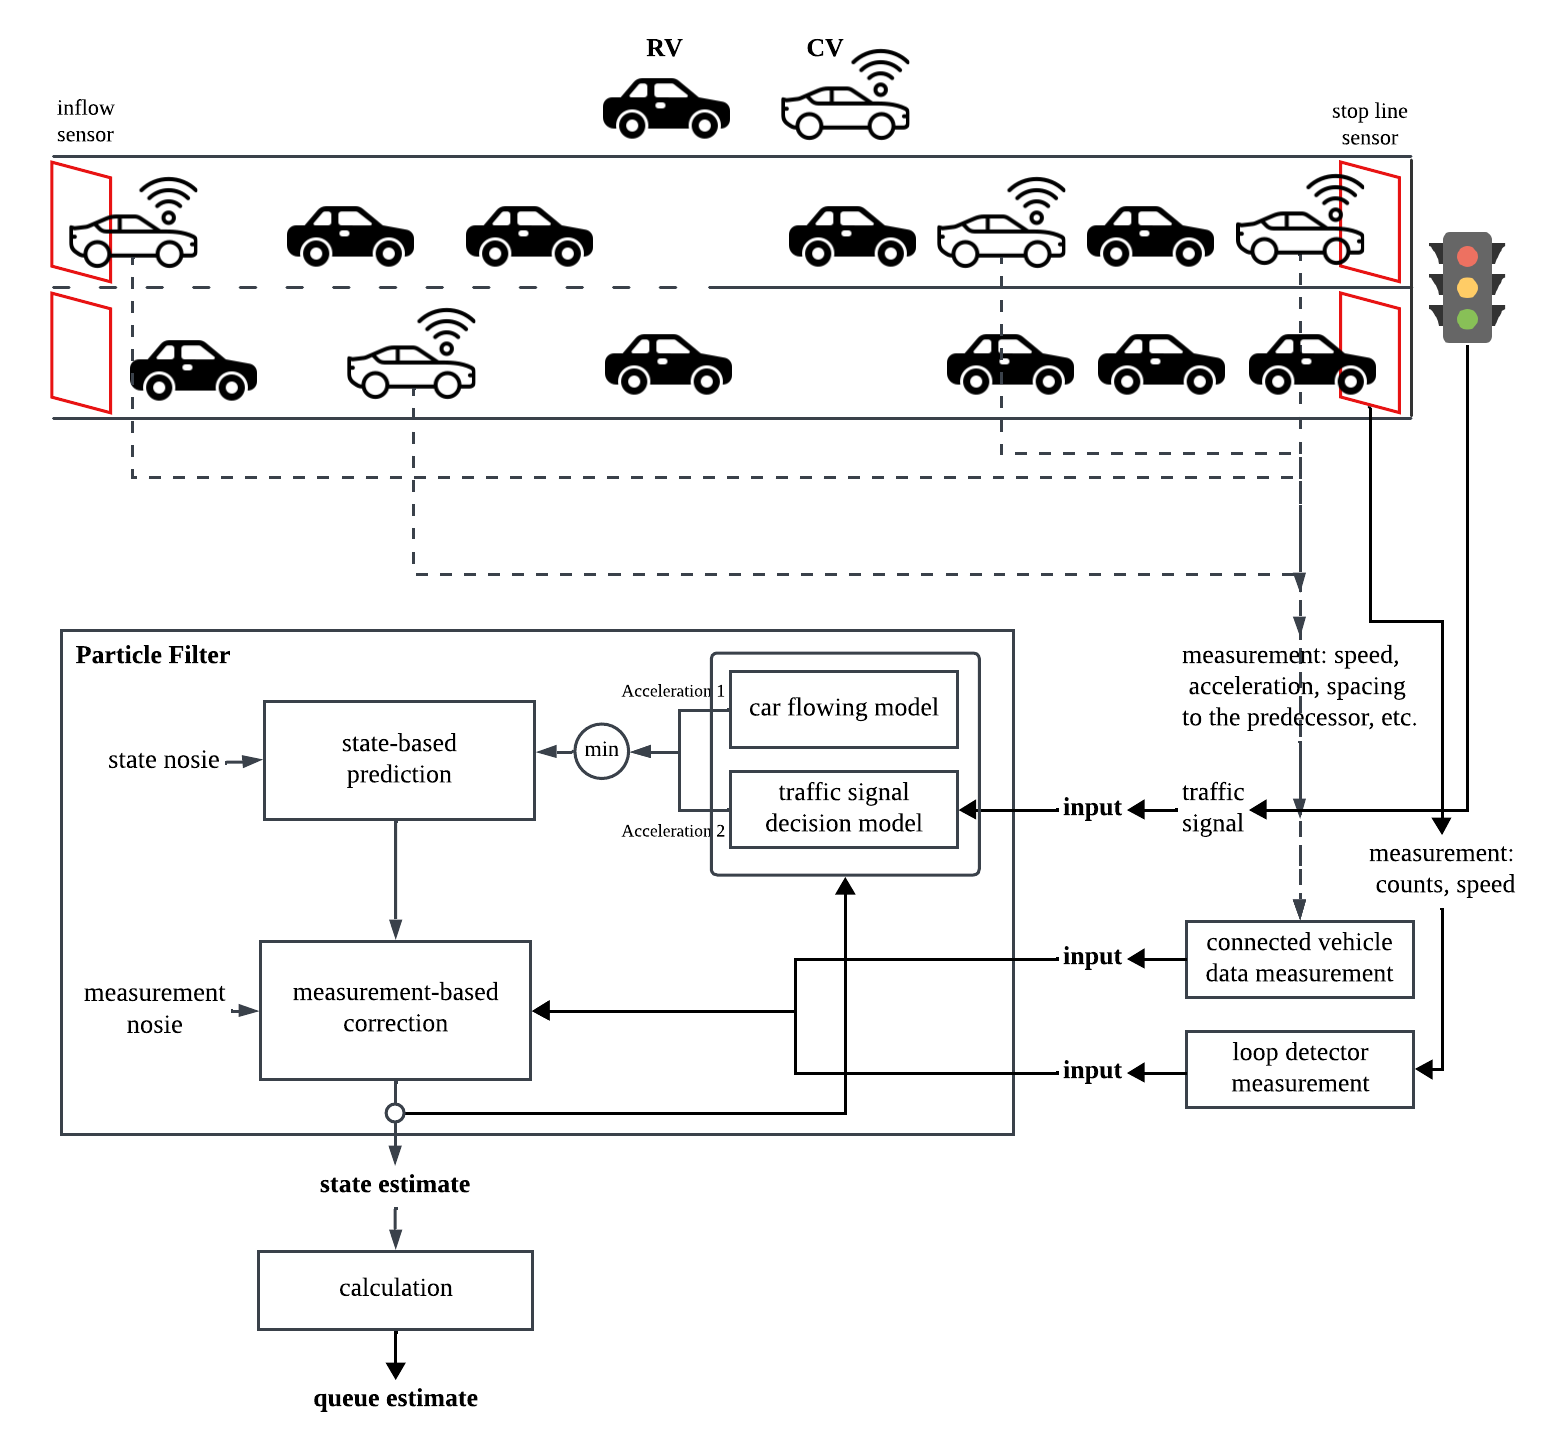
\includegraphics[width= 0.85\linewidth]{figures/architecture(1).png}
    \caption{PF-SIQE Architecture}
    \label{fig: PF-SIQE Architecture}
\end{figure}

Figure \ref{fig: PF-SIQE Architecture} illustrates the layout of a two-lane road as an example to demonstrate the particle filter framework known as PF-SIQE. This example merely explains the framework's functionality; the PF-SIQE is designed to be adaptable and applicable to various road configurations and conditions, emphasizing its generic nature and broad applicability. In this illustrative framework, connected vehicles function as floating sensors, and loop detectors act as roadside sensors to showcase the system. The framework is inherently modular, the measurement-based correction module can integrate various types of sensors beyond connected vehicles and loop detectors, highlighting its flexibility to adapt to different sensor technologies.

In this example framework, 'CV' represents connected vehicles, while 'RV' denotes regular vehicles. Assume that the CVs are equipped with GPS, providing noisy measurements at each time step, including current speed $v_k$, longitudinal distance to the stop line $d_k$, and acceleration $a_k$. LiDAR equipment on CVs measures the distance to the preceding vehicle $s_k$, as well as relative speed $\Delta v_k$ and relative acceleration $\Delta a_k$. Initially, the state transition function calculates predicted states: longitudinal position $d_{k}$, speed $v_k$, acceleration $a_k$, spacing $s_k$, lane position (lateral) $i_k^{\text{lane}}$, dilemma zone delineation ($d_a, d_b$), and decision-making processes $D_{k}$, based on previous time step prediction and the traffic signal state $S_{\text{signal}}$. These state variables are calculated by the state-based prediction module, which is one of the three principal components of the particle filter framework. To showcase the system, this module integrates the car-following model and the traffic signal decision model, both of which compute acceleration values through state transition functions. The minimum of these two acceleration values is selected and augmented with a noise term to reflect inherent system disturbances like wind resistance, road curvature, and gradients. The adjusted acceleration rate and the noise term are then used to calculate the vehicle’s speed and longitudinal position.

On the other hand, the measurement-based correction module leverages data from both the loop detector and the CVs in Figure \ref{fig: PF-SIQE Architecture}. Measurement noise is added to the data obtained from both the loop detector and the CVs. This module constructs the discrete probability function based on loop detectors' manufacturer specifications. The noise distribution in the CV measurements will be detailed in Section \ref{Measurement Function}. The joint probability is determined by taking the product of the probabilities from both data sources.

The state transition function's predictions act as the baseline for estimations. These predictions are then adjusted in a correction step through weight adjustments within the particle filter algorithm once the noisy measurements are received from CVs and additional data from loop detectors, such as vehicle counts $c_k$ and speed $v_k$.

Next, the particle filter algorithm will be introduced.


\section{Introduction to the Particle Filter Algorithm}\label{Introduction to the Particle Filter Algorithm}

The particle filter algorithm (\textcite{arulampalam2002tutorial}) is a sequential Monte Carlo method used for estimating the state of a system, where the system's state space model generates actual states, and a measurement function utilizes these measurements for correction. This section provides an overview of the key elements of the particle filter, focusing on its practical application, which sets the foundation for Section \ref{State Transition Function} and Section \ref{Measurement Function}.

\subsection{Pseudocode of the Particle Filter Algorithm}
\begin{algorithm}
\caption{Particle Filter Algorithm}\label{Particle Filter Algorithm}
\begin{algorithmic}[1]  % The [1] option enables line numbers
    \State \textbf{Input:} $\{x_{k-1}^{j}, w_{k-1}^{j}\}_{j = 1}^N, z_k$
    \State \textbf{Output:} $\{x_k^{j}, w_k^{j}\}_{j = 1}^N$
    \For{$j = 1$ \textbf{to} $N$}
        \State Draw $x_k^{j}$ from $q(x_k | x_{k-1}^{j}, z_k)$ \Comment{Typically, $q(x_k | x_{k-1}^{j}, z_k) = p(x_k | x_{k-1}^{j})$}
        \State Update weight: $\tilde{w}_k^{j} = p(z_k | x_k^{j}) w_{k-1}^{j}$
    \EndFor
    \State Normalize weights: $w_k^{j} = \frac{\tilde{w}_k^{j}}{\sum_{j=1}^N \tilde{w}_k^{j}}$
    \If{$\frac{1}{\sum_{j=1}^N (w_k^{j})^2} < N_{\text{threshold}}$}
        \State Resample particles
    \EndIf
\end{algorithmic}
\end{algorithm}
Where
\begin{itemize}
    \item $j$ is the index of the particle.
    \item $k$ is the time step.
    \item $N$ is the number of particles.
    \item $x_k^{j}$ is the state of the $j^\text{th}$ particle at time step $k$.
    \item $\tilde{w}_k^{j}$ is the intermediate weights.
    \item $w_k^{j}$ is the true weights of the new particles after the normalization process.
    \item $z_k$ is the measurement at time step $k$.
    \item $p(x_k | x_{k-1})$ is the state transition probability distribution function, which will be given in Section \ref{State Transition Probability Function}.
    \item $q(x_k | x_{k-1}^{j}, z_k)$ is the importance density function, also called the q function, when the q function is unknown, let it equal to $p(x_k | x_{k-1})$ is also a good choice typically.
    \item $p(z_k | x_k^{j})$ is the likelihood of the measurement given the state of the $j^\text{th}$ particle at time step $k$, which will be given in Section \ref{Measurement Probability Distribution Function}.
    \item $N_{\text{threshold}}$ is the threshold for the effective number of particles to decide when to resample.
\end{itemize}

In particle filters, the process of recursive estimation involves updating the particles' states and their corresponding weights based on new measurements as they become available.  The posterior distribution \( p(x_{k} | z_{1:k}) \) is approximated by a weighted set of particles \((x_{k}^{j}, w_k^{j})_{j=1}^N\), where \( \sum_{j=1}^N w_k^{j} = 1 \). Start with an initial set of particles and weights \((x_0^{j}, w_0^{j})\) at time step \(0\). When moving to the next time step, assume that the thesis knows the states and weights from the previous time step \((x_{k-1}^{j}, w_{k-1}^{j})\). The objective is to update these particles and weights to reflect the new information provided by the latest measurement \(z_k\) and the knowledge of the process dynamics.

The particle filter algorithm involves the following steps:
\begin{enumerate}
    \item Initialization: Assume the number of particles \( N \). Each particle represents a hypothetical state \( x_k \) of all the vehicles and their weight. The initial states are randomly generated, and each particle is assigned an equal weight \( w_0^{j} = \frac{1}{N} \). State $x_k$ includes various variables such as the distance to the stop line $d_k$ (longitudinal position), current speed $v_k$, acceleration $a_k$, lane position $i_k^{\text{lane}}$ (lateral position), spacing to the preceding vehicle $s_k$, dilemma zone ($d_a, d_b$), decision $D_{k}$, etc. 
    \item Prediction (Drawing Particles): The first step in the recursive estimation process is to predict the new states of the particles based on the state transition model. For each particle \(j\), a new state \(x_k^{j}\) is drawn from the importance density function \(q(x_k | x_{k-1}^{j}, z_k)\). Typically, when the exact importance density function is unknown, use the state transition probability \(p(x_k | x_{k-1})\) as an approximation. This step incorporates the system dynamics and the state noise to simulate the possible states at the new time step.
    \item Weight Update: Update the weight of each particle using the likelihood of the observed measurement \( z_k \):
      \begin{equation}
          \tilde w_k^{j} = \frac{p(z_k | x_k^{j}) p(x_k^{j} | x_{k-1}^{j})}{q(x_k | x_{k-1}^{j}, z_k)} w_{k-1}^{j}
      \end{equation}
      Since typically choose \(q(x_k | x_{k-1}^{j}, z_k) = p(x_k | x_{k-1})\), the weight update equation simplifies to:
      \begin{equation}
          \tilde w_k^{j} = p(z_k | x_k^{j}) w_{k-1}^{j}
      \end{equation}
      This means the intermediate normalized weight \(\tilde w_k^{j}\) is the product of the likelihood of the measurement \(p(z_k | x_k^{j})\) and the previous weight \(w_{k-1}^{j}\).
    \item Normalization: To ensure the weights form a valid probability distribution, they need to be normalized. This is done by dividing each weight by the sum of all weights:
      \begin{equation}
          {w}_k^{j} = \frac{\tilde w_k^{j}}{\sum_{j=1}^N \tilde w_k^{j}}
      \end{equation}
      This normalization ensures that the sum of all weights equals one.
    \item Resampling: Over time, some particles may end up with very low weights, while a few might dominate with high weights, leading to particle degeneracy. To address this, perform resampling when the effective number of particles \(N_{\text{eff}}\) falls below a certain threshold \(N_{\text{threshold}}\). The effective number of particles is estimated as:
    \begin{equation}\label{eq: effective number of particles}
        \widehat{N^{eff}} = \frac{1}{\sum_{j=1}^N ({w}_k^{j})^2}
    \end{equation}
    If \(\widehat{N^{\text{eff}}} < N_{\text{threshold}}\), resampling is triggered. In systematic resampling (see Section \ref{Systematic Resampling}), new particles are selected based on the cumulative distribution function of the normalized weights. This process ensures that particles with higher weights are more likely to be selected multiple times, while those with lower weights might be discarded. After resampling, all selected particles are assigned equal weights.
\end{enumerate}


\subsection{State Transition Probability Distribution Function: $p(x_k | x_{k-1})$}\label{State Transition Probability Function}

The state transition function \( f_k(x_{k-1}, n_{k-1}^s) \) describes how the state evolves from one time step to the next, incorporating state noise \( n_k^\text{s} \). This transition is crucial for predicting the next state based on the current state. Section \ref{State Transition Function} will present the detailed equation of $p(x_k | x_{k-1})$.

\subsection{Measurement Probability Distribution Function: $p(z_k | x_k^{j})$}\label{Measurement Probability Distribution Function}

The measurement function \( g_k(x_k, n_k^\text{m}) \) incorporates measurement noise \( n_k^\text{m} \) and provides the likelihood of the observed measurement given the state. This likelihood function \( p(z_k | x_k) \) is essential for updating the weights of the particles, which will be presented in Section \ref{Measurement Function}.

\subsection{Importance Density Function (q-function): \textbf{$q(x_k | x_{k-1}^{j}, z_k)$}}\label{q function}

In particle filters, selecting the importance density function \( q(x_k | x_{k-1}, z_k) \) is critical for drawing new particles. A common and practical choice is the state transition function \( p(x_k | x_{k-1}) \). This selection simplifies the weight update process and is the approach adopted in this thesis.

\subsection{Systematic Resampling}\label{Systematic Resampling}

Systematic resampling is a method used in particle filters to address the issue of particle degeneracy, where over time, a few particles may carry the majority of the weight, reducing the diversity of the particle set. This resampling method ensures that particles with higher weights are more likely to be selected, while particles with lower weights are less likely to survive, thereby maintaining a diverse and representative set of particles.

Here are the steps of systematic resampling:
\begin{enumerate}
    \item Compute the Cumulative Sum of Weights: Begin by computing the cumulative sum of the normalized weights of the particles. This step forms a cumulative distribution function (CDF) that will be used to draw particles for the next iteration. Essentially, you sum the weights sequentially so that each particle’s weight is added to the sum of all previous weights.
    \item Initialize Variables:
    \begin{itemize}
        \item Generate a random starting point, which is a random number uniformly distributed between 0 and the reciprocal of the number of particles ($\frac{1}{N}$). This random starting point ensures that the particles are resampled in a systematic but random manner.
        \item Set the initial index to 1. This index will be used to track which particle is being selected during the resampling process.
    \end{itemize}
    \item Resample Particles:
    \begin{itemize}
        \item For each particle in the set, calculate a target value by adding a fixed step size to the initial random starting point. The step size is the reciprocal of the number of particles ($\frac{1}{N}$).
        \item Move through the cumulative sum of weights and select particles based on the target values. If the target value falls within the cumulative weight range of a particle, that particle is selected.
        \item Assign the state of the selected particle to a new set of particles, ensuring that particles with higher weights (which have larger cumulative sums) are more likely to be chosen.
        \item After selecting a particle, assign it an equal weight, so all particles in the new set start with the same weight.
    \end{itemize}
    \item Stop Criterion: The resampling process is completed once all $N$ particles have been resampled. This is guaranteed after exactly $N$ iterations, as each iteration selects one particle based on the target values and cumulative sum of weights. Thus, the resampling process stops when the full set of $N$ particles has been replaced in the new particle set.
\end{enumerate}



Following this introduction to the particle filter algorithm, the subsequent sections will present details on the state transition function, state noise distribution, measurement function, and measurement noise distribution, with a focus on their practical implementation within the proposed framework.


\section{State Transition Function Module}\label{State Transition Function}
To align with the research objective, the particle filter will provide as accurate as possible queue estimations despite state noise and measurement noise. In the particle filter framework, the state transition function's predictions act as the baseline for estimations. These predictions are then adjusted in a correction step through weight adjustments within the particle filter algorithm once the noisy measurements are received from sensors.

When considering which state variables to include, they should align with the models that the state transition function module aims to integrate. This alignment ensures consistency and coherence between the state variables and the models used to describe the system dynamics. To maintain the scalability and align with the research objective, the state transition function in the thesis considers a wide range of state variables of the vehicles to represent the system: 
\begin{equation}\label{state variables}
    x_k^i = \begin{bmatrix}
d_k^i & v_k^i & a_k^i  & D_{k}^i & i_k^{\text{lane}}
\end{bmatrix}
\end{equation}

where
\begin{itemize}
    \item $k$ is the time step index.
    \item $i$ is the vehicle index. Keep the direction intuitive, from upstream to downstream.
    \item $x_k^i$ is the system state for one vehicle. 
    \item $d_k^i$ [m] is the longitudinal position of the  $i^{th}$ vehicle along the road. Keep the direction intuitive, from upstream to downstream.
    \item $v_k^i$ [m/s] is the instantaneous speed.
    \item $a_k^i$ [m/s$^2$] is the instantaneous acceleration rate.
    \item $D_{k}^i$ is the decision of stop or go when facing the traffic light.
    \item $i_k^{\text{lane}}$ is the index number of which lane the vehicle is.
    %\item $s_k$ [m] is the current gap to the predecessor.
    %\item $d_a$ [m] is the downstream boundary of the dilemma zone.
    %\item $d_b$ [m] is the upstream boundary of the dilemma zone.
\end{itemize}

\subsection{Handling Multiple Vehicles}
To cope with multiple vehicles, the system state vector \( X_k \) is extended to include the state vectors of all vehicles in a selected road segment at each time step $k$:
\begin{equation}
    X_k = \begin{bmatrix}
x_k^1 \\
x_k^2 \\
\cdots \\
x_k^N 
\end{bmatrix}
= \begin{bmatrix}
d_k^1 & v_k^1 & a_k^1 & D_{k}^1 & i_k^{\text{lane}, 1}  \\
d_k^2 & v_k^2 & a_k^2 & D_{k}^2 & i_k^{\text{lane}, 2}  \\
\text{$\cdot \cdot \cdot $} \\
d_k^N & v_k^N & a_k^N & D_{k}^N & i_k^{\text{lane}, N}  \\
\end{bmatrix}
\end{equation}

where \( N \) is the total number of vehicles within a specific road segment. The thesis assumes that the total number of vehicles \( N \) is constant during the estimation process within a certain time period for a given road segment. This assumption simplifies the model by not considering vehicle arrival or departure patterns. Future work could integrate vehicle arrival distributions and departure processes for more dynamic modeling, as discussed in the final chapter.





\subsection{State Transition Function}
The state transition function describes how these state variables evolve from one time step to the next, incorporating the system's dynamics, the influence of control inputs, and the presence of noise. The state transition function expresses:

\begin{enumerate}
    \item Calculation of All States: The function provides a mathematical description of how each state variable is updated at each time step.
    \item Introduction of the State Noise Term: The function incorporates state noise \(n_k^\text{s}\) to account for the randomness and uncertainties in the system dynamics.
    \item State Probability Distribution Function: The function defines the probability distribution function \(p(x_k | x_{k-1})\), which describes the likelihood of transitioning from one state to another.
\end{enumerate}

\begin{equation}
    x_{k+1} = f(x_k, n_k^\text{s}) 
\end{equation}
\begin{equation}
    d_{k+1} = d_k + v_k \cdot T + \frac{1}{2} \cdot a_k \cdot T^2  +  n_k^\text{s}  
\end{equation}
\begin{equation}
    v_{k+1} = v_k +  a_k \cdot T +  n_k^\text{s}  
\end{equation}
\begin{equation}
    a_{k+1} = \min (\bar a_{k+1}, \tilde a_{k+1}) +  n_k^\text{s}  
\end{equation}
\begin{equation}
    i_{k+1}^{\text{lane}} = g(x_k, \text{lane change external factors})
\end{equation}

where
\begin{itemize}
    \item $T$ [s] is the time step, in the simulation detailed in Chapter \ref{chapter:Experimental Design and Analysis}, $T$ is set to 1 second.
    \item $n_k^\text{s}$ is the state noise term. In this thesis, $n_k^\text{s}$ indicates the randomness $n_k^\text{d}$ in the decision-making process and the acceleration noise $n_k^\text{a}$, which will be detailed in Section \ref{State noise distribution}.
    \item $\bar a_{k+1}$ [m/s$^2$] is the acceleration rate involving the car-following model, detailed in Section \ref{car-following model: IDM}.
    \item $\tilde a_{k+1}$ [m/s$^2$] is the acceleration rate involving traffic signal status, detailed in Section \ref{Longitudinal}.
    %\item $f(a_{\text{max}}, v_k, v_{\text{desired}}, \delta, \Delta v_k, s_0, h_s, b, s_k, d_a, d_b, S_{\text{signal}}, D_{k})$ is a function that updates the acceleration based on current acceleration and external factors such as the distance to the predecessor, traffic signal status, etc. This will be addressed in the next Section \ref{Longitudinal}.
    \item $g(x_k, \text{lane change external factors})$ is a function that updates the lane position based on the current lane position and any lane change external factors, such as the surrounding vehicles, the road layout, lane change intention, or the route information.
    %\item The calculation of $s_k,  d_a,  d_b,  D_{k}$ is presented in Section \ref{Longitudinal}.
\end{itemize}
The process will occur in two phases: initially, the car-following and traffic signal decision models (so-called traffic light acceleration/deceleration models) will be applied to update the longitudinal state as a vehicle approaches a traffic signal. In future work, the lane change model may be incorporated to accurately represent lateral movements, enhancing the realism of the vehicle's behavior at intersections.


\subsection{Phase 1: Longitudinal Motion}\label{Longitudinal}
Given that the PF-SIQE primarily targets queue estimation near traffic signals, it is crucial to consider vehicle behavior (i.e. acceleration or deceleration) in response to the predecessor as well as the traffic signals when approaching and exiting the intersection. The particle filter framework is highly versatile and capable of integrating a variety of models, not limited to microscopic traffic flow models. To illustrate this versatility, this section presents the mathematical description of the integration of the car-following model and the traffic signal decision model and focuses on the calculation of $a_{k+1} = \min (\bar a_{k+1}, \tilde a_{k+1}) +  n_k^\text{s}$. The Intelligent Driver Model (IDM) from \textcite{treiber2000congested} is chosen as the car-following model in this thesis to capture the dynamic between vehicles longitudinally. Meanwhile, the traffic signal decision model is modified based on the bike acceleration/deceleration model presented by \textcite{dabiri2020optimized} to simulate the driver's response to the traffic signal. These models will be implemented in Chapter \ref{chapter:Experimental Design and Analysis} Experimental Simulation to demonstrate their effectiveness within the PF-SIQE framework.


\subsubsection{Car-Following Model: Intelligent Driver Model (IDM)}\label{car-following model: IDM}

\begin{table}[htbp]
\small
    \centering
    \begin{tabular}{cccccc}
    \toprule
         & desired  & maximum   & comfortable   & minimum   & safe time   \\
         name & speed  &  acceleration  &  deceleration  &  gap  &  headway  \\
         & \(v_{\text{desired}}\) (m/s) & $a_{\text{max}}$ (m/s$^2$)& $b$ (m/s$^2$) & $s_0$ (m) & $h_s$ (s) \\
        \hline
         value & 15.0 & 1.0 & 1.5 & 2.0 & 1.0 \\
         \toprule
    \end{tabular}
    \caption{The parameters of IDM (\textcite{treiber2013traffic})}
    \label{parameters of IDM}
\end{table}


There are plenty of car-following models developed in the previous studies. Note that the state transition function module is flexible and versatile to replace any other car-following models or lane change models with the chosen one in this thesis. \textcite{treiber2000congested} presented the Intelligent driver model(IDM), which calculates the current acceleration \(a\) by multiplying \(a_{\text{max}}\) with an adjustment factor. This adjustment factor takes into account the desired speed $v_{\text{desired}}$, the current speed $v_k$, and the current gap to the predecessor $s_k$, to simulate the driver's response to the predecessor:

\begin{equation}\label{acceleration update equation 1}
     \bar a_{k+1}  = a_{\text{max}} \left( 1 - \left( \frac{v_k}{v_{\text{desired}}} \right)^\delta - \left( \frac{s_k^*(v_k, \Delta v_k)}{s_k} \right)^2 \right) 
     %f(a_{\text{max}}, v_k, v_{\text{desired}}, \delta, \Delta v_k, s_0, h_s, b, s_k)
\end{equation}
where
\begin{itemize}
    \item \(\bar a_{k+1}\) [m/s$^2$] represents the vehicle's acceleration at time step $k+1$.
    \item \(a_{\text{max}}\) [m/s$^2$] is a model parameter that represents the maximum acceleration a vehicle can achieve under ideal conditions, reflecting the vehicle's ability to accelerate from a stationary state to its top speed.
    \item \(v_k\) [m/s] is the current speed.
    \item \(v_{\text{desired}}\) [m/s] is the desired speed, which in this case refers to the speed limit of the road segment, and is set as a model parameter. Although individual drivers may have different desired speeds, the IDM model assumes that all drivers aim to reach the maximum allowable speed, i.e., the speed limit of the road, as a simplifying assumption in this study.
    \item \(\delta\) is the free flow exponent, typically set to 4.
    \item \(s_k\) [m] is the current gap of the $i^\text{th}$ vehicle to the predecessor ${(i-1)}^\text{th}$, which can be calculated as:
    \begin{equation}
        s_k^i = d_k^{i-1} - d_k^i - l^{i-1}
    \end{equation}
    where $l^{i-1}$ is the vehicle length of the predecessor.
    \item \(\Delta v_k\) [m/s] is the relative speed to the predecessor:
    \begin{equation}
        \Delta v_k = v_k^{i} - v_k^{i-1}
    \end{equation}
    \item \(s_k^*(v_k, \Delta v_k)\) [m] denotes the desired gap, also referred to as the dynamic following distance, written as:
    \begin{equation}
    s_k^*(v_k, \Delta v_k) = s_0 + v_k h_s + \frac{v_k\Delta v_k}{2\sqrt{a_{\text{max}}b}}
    \end{equation}
    where:
    \begin{itemize}
        \item \(s_0\) [m] is the minimum gap when vehicles are stationary to ensure that collisions do not occur in a standstill situation. The specific value of \(s_0\) can be set according to the type of vehicle, traffic regulations, or driving behaviors. For instance, in some models, \(s_0\) can be set to approximately 2 m.
        \item \(h_s\) [s] refers to the safe time headway a driver wishes to maintain between themselves and the predecessor while following. In practice, \(h_s\) is often set to a value between 1 s and 2 s, to simulate driving behavior under most road conditions.
        \item \(b\) [m/s$^2$] is the comfortable deceleration rate, indicating the desired deceleration when slowing down. The value of \(b\) ranges between 1.5 to 3.0 m/s$^2$.
    \end{itemize}
\end{itemize}

Table \ref{parameters of IDM} shows the parameters of IDM. The desired speed $v_{\text{desired}} = 15 \text{ m/s}$ aligns with the common speed limit in urban areas, which is $50$ km/h. The justifications for the other parameters can be found in \textcite{treiber2013traffic}.

In the absence of a predecessor (\(s_k \rightarrow \infty\)), the acceleration for next time step \(\bar a_{k+1}\) attempts to bring the vehicle to its desired speed \(v_{\text{desired}}\). When a predecessor is present, the acceleration is influenced by two factors: the desire to reach the desired speed and the need to maintain a safe distance from the predecessor. The \(s_k^*(v_k, \Delta v_k)\) function considers the current speed, the speed difference with the predecessor, and the acceleration needed to decelerate within a safe distance, ensuring that the vehicle maintains smooth traffic flow while being capable of decelerating safely when necessary.





\subsubsection{Traffic Signal Decision Model: Acceleration/Deceleration Model}\label{Traffic Signal Decision Model: Acceleration/Deceleration Model}

Adopting a vehicle-based perspective aligns with the particle filter algorithm, shifting focus from traditional management to individual vehicle control. This approach assumes that each vehicle, whether connected or not, makes decisions based on crucial parameters such as speed limits, yellow light duration, dilemma zone boundary, reaction times, deceleration rates, and the current speed. Consequently, each vehicle can determine its position relative to its dilemma zone, whether it is approaching, within, or past it. If the traffic signal is yellow, vehicles upstream of its dilemma zone will stop, those within its dilemma zone will make a decision to stop or go (modeled as a probabilistic decision), and vehicles downstream of its dilemma zone will continue to go. This model ensures that the particle filter framework accurately represents the decision-making process for all vehicles at traffic signals, enhancing the overall realism and effectiveness of the queue estimation process.

In the context of the vehicle and traffic signal interaction, the essence of our investigation centers on how vehicles autonomously respond to traffic light changes. Emphasizing the vehicle's decision-making at traffic signals, the thesis explores the decisive moments and criteria for choosing to either stop or proceed. This analysis begins by establishing the decision-making boundary where vehicles must instantaneously respond to traffic signals, adhering to their chosen course of action.

Deciding whether to stop or go is straightforward when the traffic signal is green or red (see the decision-making model Equation \ref{decision}), but it becomes challenging when the signal is yellow. The concept of the vehicle's dilemma zone is critical in this framework, signifying a region of uncertainty faced by vehicles at a yellow light. Decision-making in this zone is influenced by several factors, including the vehicle's speed and proximity to the intersection, which dictate whether stopping or continuing is the safer option.

First, introduce the physical decision-making boundary on the road segment $D_h$: 
\begin{itemize}
    \item $D_h$ indicates the distance at which a driver begins to respond to the traffic signal, marking the initiation point for decision-making regarding the signal status.
    \item Assume the traffic signal is visible within \(D_h\). 
    \item It is assumed that once a decision is reached within the dilemma zone, it is adhered to without deviation.
    %\item Reference for brake response times for the 'first-to-stop' vehicles is made to \cite{gates2007analysis}, detailing observed 15th, 50th, and 85th percentile brake-response times as 0.7, 1.0, and 1.6 seconds, respectively.
\end{itemize}


\begin{figure}[!htbp]
    \centering
    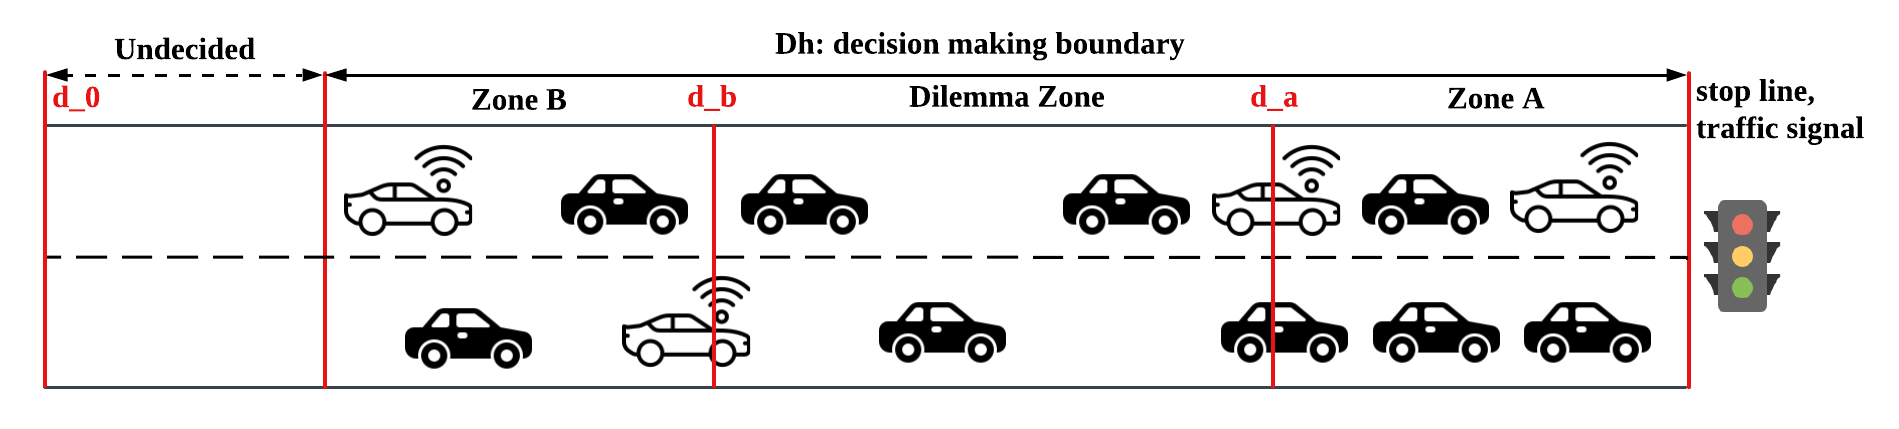
\includegraphics[width= 0.85\linewidth]{figures/dilemma zone1.png}
    \caption{Dilemma Zone}
    \label{fig: Dilemma Zone}
\end{figure}

\begin{table}[htp]
\small
    \centering
    \begin{tabular}{ccccc}
    \toprule
         &    reaction   &  deceleration   & yellow   & comfortable   \\
        name &  time  &   rate  &  time  &  acceleration  \\
         &  $T_{\text{reaction}}$ (s)& $b$ (m/s$^2$) & $T_{\text{yellow}}$ (s) & $a'$ (m/s$^2$) \\
        \hline
         value & 1.0 & 1.0 & 3.5 & 1.0 \\
         \toprule
    \end{tabular}
    \caption{The parameters of traffic signal decision model (\textcite{gates2007analysis})}
    \label{parameters of traffic signal decision model }
\end{table}
Table \ref{parameters of traffic signal decision model } shows the recommended value of the parameters in the traffic signal decision model. The justification could be found in \textcite{gates2007analysis}.

Then, present the downstream boundary $d_a$ of the vehicle's dilemma zone:

As illustrated in Figure \ref{fig: Dilemma Zone}, a vehicle requires a minimum braking distance to halt fully and securely at the stop line. This minimum braking distance defines the downstream boundary of the vehicle's dilemma zone, indicating that failing to initiate braking at this point eliminates the possibility of stopping safely and comfortably before reaching the stop line. Assume that the road gradient at the study intersection is zero (\textcite{gates2007analysis}, see equation 1),
\begin{equation}\label{downstream boundary}
    d_{a, k} = T_{\text{reaction}}v_k + \frac{v_k^2}{2b}
\end{equation}
where
\begin{itemize}
    \item $T_{\text{reaction}}$ [s] is the brake reaction time, recommended 1.0 s.
    \item $v_k$ [m/s] is the current speed.
    \item $b$ [m/s$^2$] is the deceleration rate, recommended -3.0 m/s$^2$.
\end{itemize}


Next, introduce the upstream boundary $d_b$ of the vehicle's dilemma zone:

The dilemma zone's upstream boundary indicates the location from which the stop line can just be reached if the vehicle's speed remains unchanged from the remaining time of the yellow signal to the end of the yellow signal,
\begin{equation}\label{upstream boundary}
    d_{b, k} = T_kv_k 
\end{equation}
where
\begin{itemize}
    \item $T_{\text{yellow}}$ [s] is the total yellow time, recommended 3.5 s.
    \item $T_k$ [s] is the remaining time of the yellow signal. Assume that the vehicle knows the remaining yellow time:
    \begin{equation}\label{remaining yellow time}
        T_k = T_{\text{yellow}} - T_{\text{elapsed}, k}
    \end{equation}
\end{itemize}

Deciding to go or stop is quite straightforward when the traffic light is green or red. However, the challenge arises with a yellow light. When facing a yellow light, there may be two distinct dilemma zones:
\begin{itemize}
    \item Two Options Dilemma Zone: This is the segment between \( d_a \) and \( d_b \). The downstream boundary \( d_a \) is determined by the braking distance, current speed, and deceleration rate, while the upstream boundary \( d_b \) is determined by the desired speed and the remaining yellow time. Within this dilemma zone, a vehicle could choose to stop or go, both of which are feasible options. The presence of this dilemma zone can cause confusion, especially if two longitudinally adjacent vehicles make different decisions (e.g., the predecessor chooses to stop while the successor chooses to go), creating a potential risk of collision. Therefore, modeling the randomness during the decision-making process within this two options dilemma zone is necessary.
    %\item Pitfall Zone: This is the area extending from the stop line to \( d_a \), where it is not possible to pass or stop safely. In this zone, the yellow time is too short to allow the vehicle to pass successfully at the desired speed, and the distance to the stop line is too short for a safe braking maneuver, making it impossible to stop comfortably before the stop line. This thesis assumes that the yellow time is long enough to avoid the pitfall zone.
    \item Pitfall Zone: This is the area extending between \(d_a\) and \(d_b\) when \(d_a\) is upstream of \(d_b\). In this zone, the yellow time is too short to allow the vehicle to pass successfully at the desired speed, and the distance to the stop line is too short for a safe braking maneuver, making it impossible to stop comfortably before the stop line. If \(d_b\) is more upstream, the pitfall zone extends between \(d_a\) and the stop line, where the vehicle cannot stop safely and should continue through the intersection. This thesis assumes that the yellow time is long enough to avoid the pitfall zone.
\end{itemize}

\begin{figure}[!htbp]
    \centering
    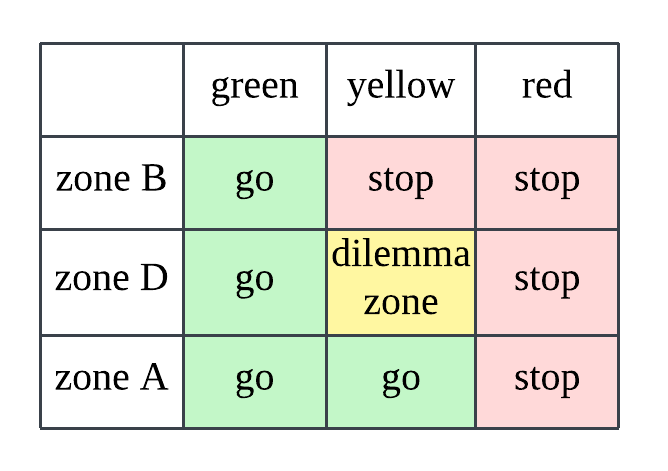
\includegraphics[width= 0.45\linewidth]{figures/decision making.png}
    \caption{Decision making}
    \label{fig: Decision making}
\end{figure}
\begin{figure}[!htbp]
    \centering
    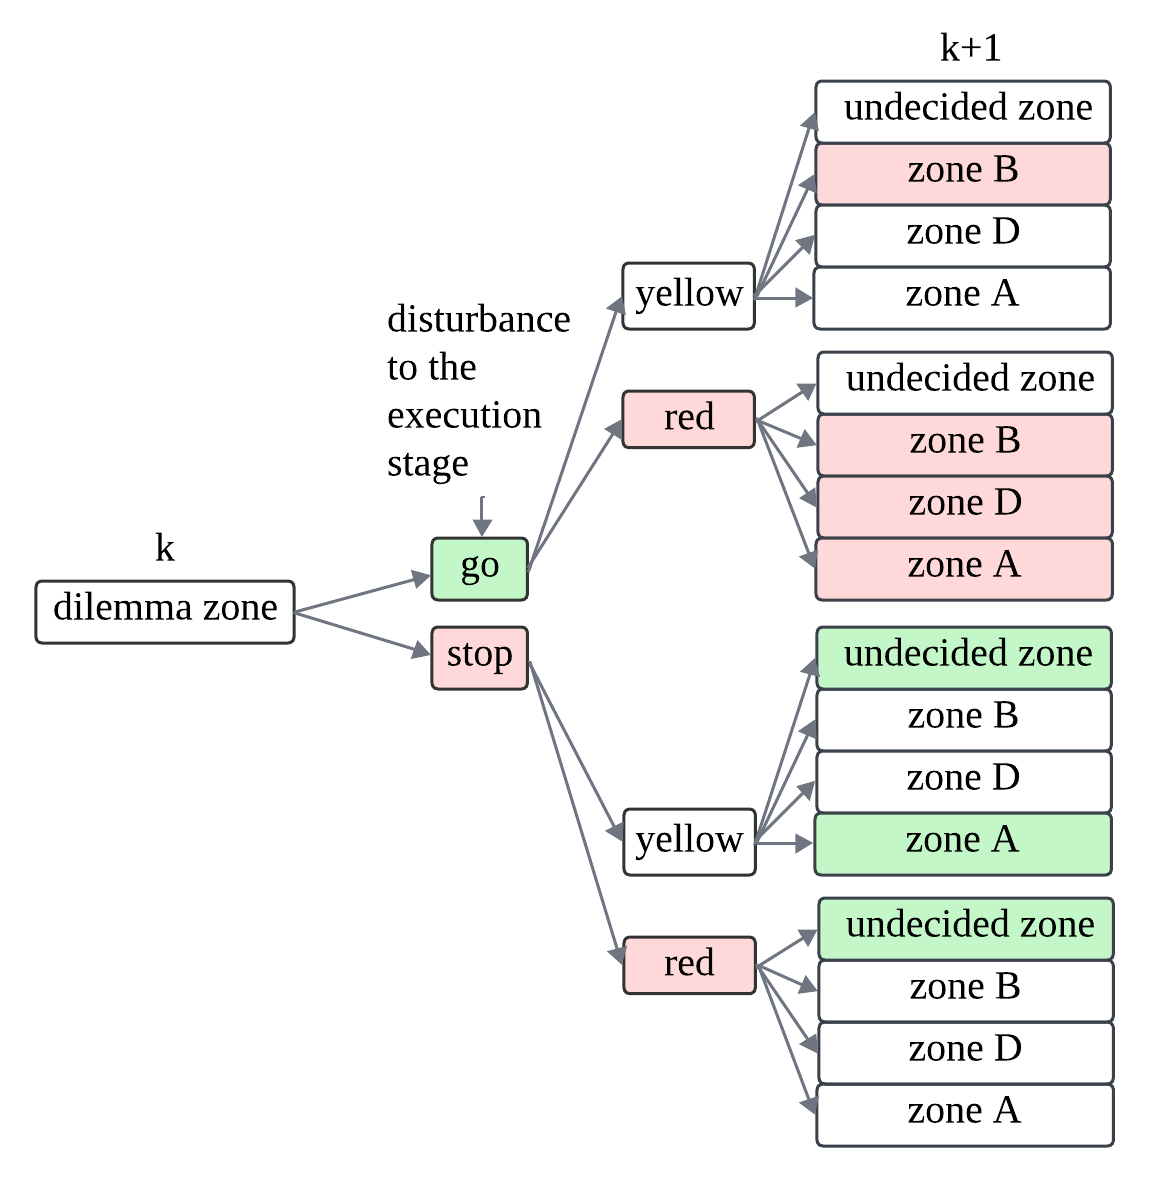
\includegraphics[width= 0.65\linewidth]{figures/decision making for dilemma zone.png}
    \caption{Decision making for dilemma zone: conflicting between $k$ and $k+1$}
    \label{fig: Decision making for dilemma zone}
\end{figure}



In Figure \ref{fig: Dilemma Zone}, Zone A is defined as the area extending from $d_a$ to the stop line $d_\text{stop line}$. Consequently, a driver has to proceed if they are in zone A when encountering a yellow light. The segment between $d_b$ and $d_a$ denotes the Two Options Dilemma Zone, where drivers are faced with the decision to either continue or halt based on a predefined probability distribution. Zone B stretches from $D_h$ to $d_b$, indicating a region where the default action for drivers is to stop. In summary, when a vehicle approaches from upstream of the traffic signal (Figure \ref{fig: Decision making}):
\begin{itemize}
    \item If the signal status is red ($S_{k+1} = S_{\text{red}}$), the decision is to stop, $D_{k+1} = D_{\text{stop}}$.
    \item If the signal status is green ($S_{k+1} = S_{\text{green}}$), the decision is to maintain speed according to the car-following model, $D_{k+1} = D_{\text{go}}$.
    \item If the signal status is yellow ($S_{k+1} = S_{\text{yellow}}$):
    \begin{itemize}
        \item If the vehicle is in Zone B ($D_h \leq d_{k+1} \leq d_{b, k+1}$), the decision is to stop, $D_{k+1} = D_{\text{stop}}$.
        \item If the vehicle is in Zone A ($d_{a, k+1} \leq d_{k+1} \leq d_\text{stop line}$), the decision is to proceed, $D_{k+1} = D_{\text{go}}$. 
        \item Figure \ref{fig: Decision making for dilemma zone} illustrates the exceptions to adhering to decisions within the dilemma zone. For instance, if a vehicle is within its dilemma zone and decides to proceed at time step \(k\), it might face disturbances during the execution stage, such as the predecessor slowing down. Consequently, at \(k+1\), if the traffic signal remains yellow, the vehicle might end up in Zone B. According to Figure \ref{fig: Decision making}, in the (yellow, Zone B) scenario, the decision should be to stop. Therefore,
        \begin{itemize}
            \item If both at time step $k$ and $k+1$, the vehicle is within its dilemma zone, particles will adhere to a probability distribution to either pass or stop and once decided, the vehicle will stick to this decision.
            \item If at time step $k$ the vehicle is within its dilemma zone, while at time step $k+1$ the vehicle is not within the dilemma zone, the vehicle will not stick to the decision at time step $k$.
            \item In conclusion, if and only if both at time step $k$ and $k+1$, the vehicle is within its dilemma zone, the vehicle will stick to the decision.
        \end{itemize}
    \end{itemize} 
\end{itemize}

For the dilemma zone, introduce a discrete probability distribution to model the vehicle's decision-making process in its dilemma zone. Define the probability of stopping as follows:

\begin{equation}
    p(D_{\text{stop}} | S_{\text{yellow}}, D_\text{undecided}, d_{b, k+1} < d_{k+1} < d_{a, k+1}) = p
\end{equation}

Thus, the probability of going is:

\begin{equation}
    p(D_{\text{go}} | S_{\text{yellow}}, D_\text{undecided}, d_{b, k+1} < d_{k+1} < d_{a, k+1}) = 1 - p
\end{equation}

where:
\begin{itemize}
    \item \(p\) is the probability that the vehicle chooses to stop when facing a yellow light in its dilemma zone.
\end{itemize}

Therefore, the decision $D_{k+1}^i$ of the $i^{th}$ individual vehicle responding to the signal status can be defined as a state-space model:
\begin{equation}\label{decision}
    D_{k+1}^i = 
\begin{cases} 
D_{\text{undecided}}, & \text{if } d_0 \leq d_{k+1} \leq D_h \text{ (undecided zone) },\\
D_{\text{stop}}, &  \begin{cases}
    \text{if } D_h \leq d_{k+1} \leq d_\text{stop line} \text{ (decided zone)}, S_{k+1} = S_{\text{red}}, \\
    \text{if } D_h \leq d_{k+1} \leq d_{b, k+1} \text{ (zone B)}, S_{k+1} = S_{\text{yellow}}, \\
    \text{if } d_{b, k+1} < d_{k+1} < d_{a, k+1} \text{ (dilemma zone)}, S_{k+1} = S_{\text{yellow}}, \\D_k = D_\text{undecided} \text{ or } d_k \text{ is out of dilemma zone},\text{and } p_\text{stop} = p, \\
\end{cases} \\
D_{\text{go}}, & \begin{cases}
    \text{if } D_h \leq d_{k+1} \leq d_\text{stop line} \text{ (decided zone)}, S_{k+1} = S_{\text{green}}, \\
    \text{if } d_{a, k+1} \leq d_{k+1} \leq d_\text{stop line} \text{ (zone A)}, S_{k+1} = S_{\text{yellow}}, \\
    \text{if } d_{b, k+1} < d_{k+1} < d_{a, k+1} \text{ (dilemma zone)}, S_{k+1} = S_{\text{yellow}}, \\D_k = D_\text{undecided}\text{ or } d_k \text{ is out of dilemma zone}, \text{and } p_\text{go} = 1 - p, \\
\end{cases} \\
D_{k}^i, & \text{if and only if both at time step $k$ and $k+1$, the vehicle is within its dilemma zone}.
\end{cases}
\end{equation}
First, during initialization, when the vehicle approaches from upstream towards the traffic signal and \(d_0 \leq d_{k+1} \leq D_h\), the initial decision has not yet been made, denoted as \(D_{k+1} = D_{\text{undecided}}\). The state \(D_{\text{undecided}}\) ensures that the vehicle can dynamically update its decision based on the signal status and its position relative to its dilemma zone. Once the decision is made at time step $k$, the vehicle will adhere to this decision in subsequent time steps, meaning $D_{k+1}^i = D_{k}^i$ if the decision has already been made at the time step $k$. This state-space model allows the decision-making process to be dynamically updated based on the vehicle's previous decision and the current signal status, ensuring consistency in the vehicle's behavior once a decision has been made.

Here is the pseudocode for the decision-making process of vehicles at traffic signals: Algorithm \ref{Traffic Signal Decision-Making Algorithm}.
\begin{algorithm}[htp]
\caption{Traffic Signal Decision-Making Algorithm}\label{Traffic Signal Decision-Making Algorithm}
\begin{algorithmic}[1]  % The [1] option enables line numbers
    \State \textbf{Input:} $d_k^i, d_{k+1}^i, v_k^i, v_{k+1}^i, S_k, S_{k+1}, T_k^i, T_{k+1}^i, D_k^i, p$
    \State \textbf{Output:} $D_{k+1}^i$
    \State \textbf{Constants:} $D_h = 150$, $T_{\text{reaction}} = 1.0$, $b = 3.0$, $T_{\text{yellow}} = 3.5$
    \For{$i = 1$ \textbf{to} $N$}
        \If{$d_0 \leq d_{k+1}^i \leq D_h$}
            \State $D_{k+1}^i = D_{\text{undecided}}$
        \Else
            \If{$S_{k+1} = S_{\text{red}}$}
                \If{$D_h \leq d_{k+1}^i \leq d_\text{stop line}$}
                    \State $D_{k+1}^i = D_{\text{stop}}$
                \EndIf
            \ElsIf{$S_{k+1} = S_{\text{green}}$}
                \If{$D_h \leq d_{k+1}^i \leq d_\text{stop line}$}
                    \State $D_{k+1}^i = D_{\text{go}}$
                \EndIf
            \ElsIf{$S_{k+1} = S_{\text{yellow}}$}
                \State Calculate downstream boundary $d_{a, k+1}^i = T_{\text{reaction}} \cdot v_{k+1}^i + \frac{(v_{k+1}^i)^2}{2 \cdot b}$
                \State Calculate remaining yellow time $T_{k+1}^i = T_{\text{yellow}} -T_{\text{elapsed}, {k+1}}^i$
                \State Calculate upstream boundary $d_{b, k+1}^i = T_{k+1}^i \cdot v_{k+1}^i$
                \If{$D_h \leq d_{k+1}^i \leq d_{b, k+1}^i$}
                    \State $D_{k+1}^i = D_{\text{stop}}$
                \ElsIf{$d_{a, k+1}^i \leq d_{k+1}^i \leq d_\text{stop line}$}
                    \State $D_{k+1}^i = D_{\text{go}}$
                \ElsIf{$d_{b, k+1}^i < d_{k+1}^i < d_{a, k+1}^i$}
                \State Calculate boundaries at time step $k: d_{b, k}^i, d_{a, k}^i$
                    \If{$d_{a, k}^i \leq d_k^i, d_k^i \leq d_{b, k}^i$ \textbf{or} $D_k^i = D_{\text{undecided}}$} 
                        \State Generate a random value $r \sim \mathcal{U}[0, 1]$
                        \If{$r < p$}
                            \State $D_{k+1}^i = D_{\text{stop}}$
                        \Else
                            \State $D_{k+1}^i = D_{\text{go}}$
                        \EndIf
                    \EndIf
                \EndIf
            \EndIf
        \EndIf
        \If{$S_k = S_{k+1} = S_{\text{yellow}}$ \textbf{and} $D_{k}^i = D_{\text{decided}}$}
            \State Calculate boundaries at $k$ and $k+1$: $d_{b, k}^i, d_{a, k}^i, d_{b, k+1}^i, d_{a, k+1}^i$
            \If{$d_{b, k}^i < d_k^i < d_{a, k}^i$ \textbf{and} $d_{b, k+1}^i < d_{k+1}^i < d_{a, k+1}^i$}
                \State $D_{k+1}^i = D_k^i$ \Comment{Maintain the previous decision if already made}
            \EndIf
        \EndIf
    \EndFor
\end{algorithmic}
\end{algorithm}






Next, determine the state update function of acceleration.
The model for vehicle acceleration and deceleration at intersections, influenced by traffic signal status, is adapted from a stochastic dynamic programming approach originally developed for cyclists by \textcite{dabiri2020optimized}. Given the significant differences in dynamics between vehicles and bicycles, special attention is given to adjusting the acceleration parameters within the model to accurately reflect the distinct acceleration and deceleration capabilities of motor vehicles. 


\begin{equation}\label{acceleration update equation 2}
     \tilde a_{k+1} = 
\begin{cases} 
-\frac{v_k}{C_{s,k} \cdot T}, & \text{if } D_k = D_{\text{stop}}, \\
0, & \text{if } D_k = D_{\text{go}}, v_k > v_{\text{desired}}, \\
a' \left(1 - \left(\frac{v_k}{v_{\text{desired}}}\right)^2\right), & \text{Otherwise}
\end{cases}
\end{equation}


where:
\begin{itemize}
    \item \(\tilde a_k\) [m/s$^2$]: The vehicle's acceleration/deceleration at time step \(k\).
    \item \(v_k\) [m/s]: The speed of the vehicle at time step \(k\).
    \item \(C_{s,k}\) : The number of required time steps at time step \(k\) for the vehicle to fully stop before the intersection, written as:
    \begin{equation}
        C_{s,k} = \max \left(1, \frac{2d_k}{v_k T}\right)
    \end{equation}
    where \(d_k\) [m]: The distance between the vehicle and the stop line (traffic signal) at time step \(k\).
    \item \(T\) [s]: The discretization time interval, set as 1 s.
    \item \(D_h\) [m]: The distance where the driver begins to make the decision and respond to the signal.
    \item \(a'\) [m/s$^2$]: The comfortable acceleration of the vehicle, recommended 1.0 m/s$^2$.
    \item \(v_{\text{desired}}\) [m/s]: The desired speed of the vehicle.
\end{itemize}
Therefore, combining the $\bar a_{k+1}$ (equation \ref{acceleration update equation 1}) and the $\tilde a_{k+1}$ (equation \ref{acceleration update equation 2}), with introducing the acceleration noise $n_k^\text{a}$, the longitudinal acceleration rate can be written as:
\begin{equation}
    a_{k+1} = \min \left(\bar a_{k+1}, \tilde a_{k+1}\right) + n_k^\text{a}
\end{equation}


\subsubsection{State Noise Distribution}\label{State noise distribution}
State noise is an essential component in modeling the uncertainties in the decision-making process. The randomness inherent in this process can be represented as:
\begin{equation}
    D_{k+1} = f (D_k, n_k^\text{d})
\end{equation}
The probability distribution function $p(D_{k+1}|D_k)$ is defined as:
\begin{equation}
p(D_{k+1}^i | D_k^i) =
\begin{cases}
1, & \text{if } D_{k+1}^i = D_k^i, \\
p, & \text{if } S_{k+1} = S_{\text{yellow}}, d_{b, k+1} < d_{k+1} < d_{a, k+1}, D_k^i = D_{\text{undecided}} \text{ and } D_{k+1}^i = D_{\text{stop}}, \\
1 - p, & \text{if } S_{k+1} = S_{\text{yellow}}, d_{b, k+1} < d_{k+1} < d_{a, k+1}, D_k^i = D_{\text{undecided}} \text{ and } D_{k+1}^i = D_{\text{go}}. 
\end{cases}
\end{equation}

To accurately model the state transition function, it is necessary to introduce noise into the acceleration and decision-making processes. Including acceleration noise is particularly significant, as it accounts for various real-world factors such as wind, gradient, road curvature, and surface friction.

Assuming that the acceleration noise follows a dissymmetrical uniform distribution $n_k^\text{a} \sim \mathcal{U}[-\frac{v_k}{T}n^\text{a}, n^\text{a}]$, the noise distribution can be described as:\\
$\bar a_{k+1} = f(a_k),$
$\tilde a_{k+1} = f(a_k),$
\begin{equation}\label{The acceleration noise probability function}
p(a_{k+1}|a_k) = \begin{cases} 
(1+\frac{v_k}{T})n^\text{a}, & \text{for } \min \left(\bar a_{k+1}, \tilde a_{k+1}\right) - \frac{v_k}{T}n^\text{a}  \leq a_{k+1} \leq \min \left(\bar a_{k+1}, \tilde a_{k+1}\right) + n^\text{a} \\
0, & \text{otherwise} 
\end{cases}
\end{equation}
This thesis assumes that the acceleration noise follows a uniform distribution due to the diverse factors influencing it. While the exact distribution of acceleration noise remains a complex issue, this assumption simplifies the model and allows the thesis to proceed with practical estimations.

\subsubsection{Probability Distribution Function of the State Noise}
To comprehensively model the state transition function, it is crucial to consider both acceleration and the decision-making process as sources of state noise. Despite the physical relations between acceleration and speed, and between speed and location being noiseless, this thesis introduce noise to acceleration to account for unpredictable variations in driver behavior and external factors. This approach captures the stochastic nature of real-world driving, ensuring a more realistic model. The combined effect of noise from acceleration and the decision-making process can be represented by the joint probability distribution function of the state noise:
\begin{equation}
    p(x_{k+1}|x_k) = p(a_{k+1}|a_k) \cdot p(D_{k+1}|D_k)
\end{equation}
By incorporating both the acceleration noise and the decision-making noise, the model provides a more accurate representation of the uncertainties in the system. This joint probability distribution function captures the combined influence of these factors, ensuring that the particle filter framework can effectively estimate the state transitions in the presence of real-world variability.

\subsection{Phase 2: Lateral Motion}\label{Lateral}
The study of lateral motion $g(x_k, \text{lane change external factors}, n_k^\text{lateral})$, integrating essential road layout factors (number of lanes, types of lanes such as through lanes, dedicated turning lanes, turning pockets, bus lanes, etc., and direction), interaction with surrounding vehicles, and the lane change model will be briefly discussed in Chapter \ref{chapter: Discussion, Conclusion, and Recommendation}. 

To incorporate lane-change decision noise, it is assumed that the lane-change decision process and all state noises are independent. This assumption allows the independent probabilities to be combined by taking their product. If there is a need to include additional microscopic traffic flow models such as the lane-change model, the joint probability distribution function can be extended as follows:
\begin{equation}
p(x_{k+1}|x_k) = p(a_{k+1}|a_k) \cdot p(D_{k+1}|D_k) \cdot p(i_{k+1}^{\text{lane}}|i_{k}^{\text{lane}}) \cdot \cdot \cdot \cdot
\end{equation}
This approach demonstrates the scalability, extendability, and versatility of the PF-SIQE framework.

\section{Measurement Function Module}\label{Measurement Function}
The PF-SIQE is designed to handle diverse measurement inputs by modularizing the input mechanism within its framework. This allows for the creation and integration of distinct measurement functions, each tailored with a specific noise distribution to match the variety of detector types. Depending on the available detectors (and the corresponding measurement noise characteristics they present), the PF-SIQE can call the appropriate input module within the particle filter estimator to perform accurate estimations.

The PF-SIQE framework in this thesis allows integration of all kinds of sensors existing in reality, including both roadside sensors and floating sensors, intrusive sensors and nonintrusive sensors, passive sensors and active sensors, and their various configurations. To achieve this, this section will introduce four variables to the measurement model: sensor type (e.g., $ z^\text{count loop}$, $z^\text{occupancy loop}$, $ z^\text{speed loop}$, $z^\text{GPS}$, $z^\text{camera}$, $z^\text{LiDAR}$, etc), sensor location (e.g., $d^\text{count loop}$, $d^\text{occupancy loop}$, $d^\text{speed loop}$, $d^\text{camera}$, $d^\text{LiDAR}$, etc), sensor size (e.g., loop length: $l^\text{count loop}$, $l^\text{occupancy loop}$, $l^\text{speed loop}$, etc), and detection range (e.g., $r^\text{camera}$, $r^\text{LiDAR}$, etc).

To show the scalability and adaptability of the PF-SIQE, we need to demonstrate its ability to handle different configurations. Therefore, to align with Chapter \ref{chapter:Experimental Design and Analysis}, this section will take loop detector and connected vehicle data as an example and provide the measurement function and the probability distribution function. Note that the framework is modular, thus it is not limited to loop detectors or connected vehicle data but can also accommodate other sensor configurations.

Specifically, this section will investigate the following aspects:
\begin{itemize}
    \item The measurement output of each sensor type;
    %\item The noise distribution associated with these measurements;
    \item The probability distribution function of the measurement noise.
\end{itemize}

\subsection{Measurement Function}\label{MF}
\begin{figure}[!htbp]
    \centering
    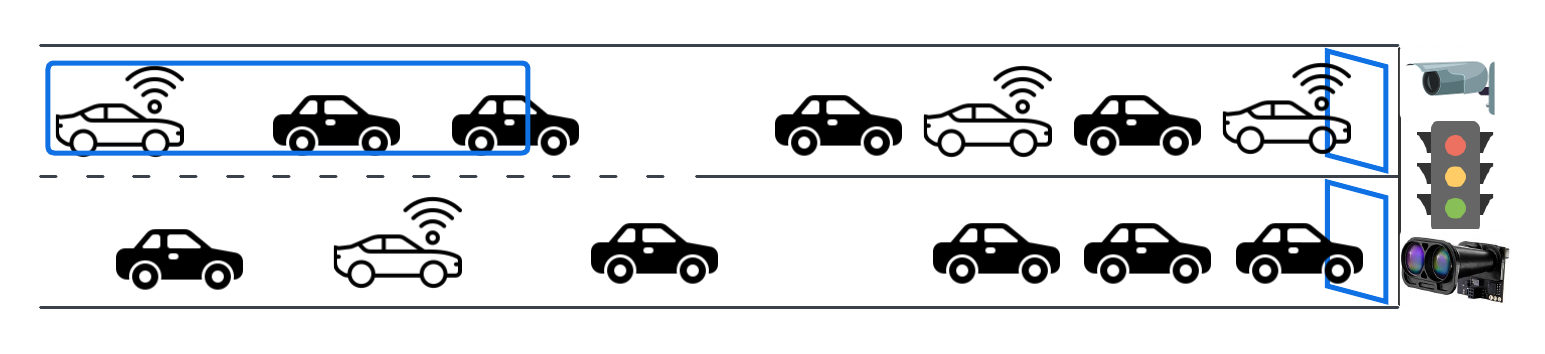
\includegraphics[width= 0.85\linewidth]{figures/sensors.png}
    \caption{Inductive loop detector, Video detection system, LiDAR, Connected vehicles}
    \label{fig: Loop detector position}
\end{figure}

Although the measurement function module in the PF-SIQE is versatile and adaptable to various sensors, it is impractical to include all sensor types within the scope of this thesis. Therefore, to demonstrate the framework's scalability and adaptability, this thesis will focus on the integration of three types of loop detectors and in-car sensors as examples. Assumptions:
\begin{itemize}
    \item The measurement outputs of loop detector $ z_k^\text{loop}$ includes
    \begin{itemize}
        \item count $\tilde c_k$ (number of vehicles passing the loop detector during time step $k$) from the count loop (i.e. loop 1). 
        \item occupancy $\tilde o_k$ (yes/ no during time step $k$) from the occupancy loop (i.e. loop 2). 
        \item average speed $\tilde v_k$ [m/s] from the speed loop (i.e. loop 3).
    \end{itemize}
    \item the placement of the loop detector is also tunable in the model, allowing it to be set as a parameter to adjust detection location based on specific road configurations.
    \item The measurement outputs of in-car sensor $z_k^\text{GPS}$ is position $\tilde d_k^i$ [m]. The $\tilde d_k^i$ contains information on the position and the corresponding vehicle ID.
    %speed $\tilde v_k^i$ [m/s], the relative speed to the predecessor $\Delta \tilde v_k^i$ [m/s], the current gap to the predecessor $\tilde s_k^i$ [m], the acceleration $\tilde a_k^i$ [m/s$^2$], the relative acceleration to the predecessor $\Delta \tilde a_k^i$ [m/s$^2$]. 
    %\item Assume the measurements from different sensors are independent.
    \item Assume that all output quantities are measured directly, and their noises are independent.
\end{itemize}


%when a GPS position $\beta(x_k)$ is near the downstream of the loop detector, which validates that a vehicle has passed the loop detector. 
The measurement function $g_k(z_k, n_k^\text{m})$: 
\begin{equation}
    z_k = \begin{bmatrix}
\text{$\tilde d_k^i$} \\
\text{$\tilde c_k$} \\
\text{$\tilde o_k$} \\
\text{$\tilde v_k$} \\
\text{$\cdot \cdot \cdot$} \\
\end{bmatrix}
= \begin{bmatrix}
\text{$f^\text{GPS}(x_k, n_k^\text{GPS})$} \\
\text{$f^\text{loop 1}(x_k, n_k^\text{loop 1})$} \\
\text{$f^\text{loop 2}(x_k, n_k^\text{loop 2})$} \\
\text{$f^\text{loop 3}(x_k, n_k^\text{loop 3})$} \\
\text{$\cdot \cdot \cdot$} \\
\end{bmatrix}
\end{equation}

where
\begin{itemize}
    \item $z_k$  denotes the measurement at time step $k$.
    \item $\tilde d_k^i$ represents the observed position of the $i$-th vehicle from in-car GPS at time step $k$.
    \item $\tilde c_k$ denotes the observed vehicle count (i.e. number of vehicles passing loop 1) at time step $k$.
    \item $\tilde o_k$ represents the observed loop occupancy from loop 2 at time step $k$.
    \item $\tilde v_k$ is the observed vehicle speed from loop 3 at time step $k$.
    \item $f^\text{GPS}(x_k, n_k^\text{GPS})$ is the function that models the GPS measurement, which is dependent on the state $x_k$ and the GPS measurement noise $n_k^\text{GPS}$.
    \item $f^\text{loop 1}(x_k, n_k^\text{loop 1})$, $f^\text{loop 2}(x_k, n_k^\text{loop 2})$, $f^\text{loop 3}(x_k, n_k^\text{loop 3})$ are functions modeling different types of loop detectors' measurements at different locations, dependent on the state $x_k$ and their respective measurement noises $n_k^\text{loop 1}$, $n_k^\text{loop 2}$, $n_k^\text{loop 3}$.
    \item The ellipses ($\cdot \cdot \cdot$) indicate that there could be additional measurements from other sensors or further configurations.
    \item $n_k^\text{m}$ is the measurement noise term. In this thesis, $n_k^\text{m}$ indicates the measurement noise from all the considered detectors, i.e. $n_k^\text{GPS}$,  $n_k^\text{loop 1}$, $n_k^\text{loop 2}$, $n_k^\text{loop 3}$, all independent.
\end{itemize}

In this framework, the measurement function $g_k(z_k, n_k^\text{m})$ aggregates the outputs from multiple sensor types, each with its respective noise distribution, into a single measurement vector $z_k$ for use in the particle filter estimation process. This modularity ensures the flexibility and adaptability of the PF-SIQE framework to various real-world sensor configurations. Next, Section \ref{Roadside sensor measurement noise distribution} and Section \ref{Floatings sensor measurement noise distribution} will investigate the measurement noise distribution from roadside sensors and floating sensors, and write the probability distribution function $p(z_k | x_k)$.

\subsection{Roadside Sensor Measurement Noise Distribution}\label{Roadside sensor measurement noise distribution}
As discussed in Section \ref{Roadside Sensor (Eulerian Sensor)}, it is crucial of extracting measurement noise distribution from the accuracy information/specification. This section will construct discrete probability distribution from the actual manufacturer's requirements. 


%As previously mentioned, the measurement outputs of $\alpha_k$ include $k, c_k^{\text{in}}, v_k^{\text{in}}, c_k^{\text{out}}, v_k^{\text{out}}$. To calculate $p(\alpha_k | x_k)$ requires a thorough examination of the noise distribution associated with $c_k$ and $v_k$. Surprisingly, this information is mentioned in the manufacturer's requirements.

\begin{table}[htp]
\centering
\begin{tabular}{p{0.8\linewidth}}
\toprule
\textbf{Vehicle Counting Accuracy} \\
\midrule
The number of vehicles counted deviates, in 95\% of the cases, by a maximum of 2\% from the actual number when a group of 1,000 vehicles passes a counting point on a lane. \\
\bottomrule
\end{tabular}

\vspace{0.1cm}

\begin{tabular}{p{0.8\linewidth}}
\toprule
\textbf{Speed Measurement Accuracy (95\% of cases)} \\
\midrule
\begin{itemize}
    \item 10\% if the speed is $\leq$ 20 km/h;
    \item 3\% if the speed is $>$ 20 km/h and $\leq$ 60 km/h;
    \item 5\% if the speed is $>$ 60 km/h and $\leq$ 180 km/h;
    \item 10\% if the speed is $>$ 180 km/h and $<$ 250 km/h.
\end{itemize} \\
\bottomrule
\end{tabular}

\vspace{0.1cm}

\begin{tabular}{p{0.8\linewidth}}
\toprule
\textbf{Speed Measurement Accuracy (remaining 5\% of cases)} \\
\midrule
\begin{itemize}
    \item 20\% if the speed is $\leq$ 20 km/h;
    \item 6\% if the speed is $>$ 20 km/h and $\leq$ 60 km/h;
    \item 10\% if the speed is $>$ 60 km/h and $\leq$ 180 km/h;
    \item 20\% if the speed is $>$ 180 km/h and $<$ 250 km/h.
\end{itemize} \\
\bottomrule
\end{tabular}
\caption{Loop detector Specifications. Source: Rijkswaterstaat, the Netherlands; translated by Henk Taale; used with permission. }
    \label{Loop detector Specifications. Source: Henk Taale, used with permission}
\end{table}

\subsubsection{Measurement Noise Distribution for Vehicle Count $\tilde c_k$ from Loop 1}
The measurement function of $\tilde c_k$ considering noise:

\begin{equation}
    \tilde c_k = c_k + n_k^\text{loop 1}
\end{equation}
\begin{equation}
    n_k^\text{loop 1} = f(c_k)
\end{equation}

\begin{equation}\label{VehicleCounting}
c_k = \sum_{i} \mathbb{I}(d_{k}^i \geq d^{\text{loop 1}}) \cdot \mathbb{I}(d_{k-1}^i \leq d^{\text{loop 1}})
\end{equation}

Where:
\begin{itemize}
    \item \(\mathbb{I}(\cdot)\) is the indicator function, which is 1 if the condition inside is true, and 0 otherwise.
\end{itemize}


To calculate the vehicle count \(c_k\) at time step \(k\) using the states \(x_k\), consider the upstream end of loop 1 \(d^{\text{loop 1}}\) and the vehicle position \(d_k^i\) with state noise. The pseudocode for calculating vehicle counts at time step \(k\) is shown below (see Algorithm \ref{Vehicle Counting Algorithm}). This algorithm initializes the count, iterates through each vehicle's position, and checks if the vehicle's position at time step \(k\) is downstream of the loop's upstream end. If so, it calculates the vehicle's position at the previous time step \(k-1\). If the position at \(k-1\) is upstream of the loop's upstream end, the vehicle is counted as having passed through the loop, and the count is incremented.

\begin{algorithm}[htp]
\caption{Vehicle Counting Algorithm for Loop 1}\label{Vehicle Counting Algorithm}
\begin{algorithmic}[1]
    \State \textbf{Input:} $d^{\text{loop 1}}, d_{k}^i$
    \State \textbf{Output:} $c_k$
    \State \textbf{Initialize:} $c_k$ $\gets 0$
    \For{$i = 1$ \textbf{to} $N$}
    %\For{$d_{k}^i$ in vehicle positions at $k$}
        \If{$d_{k}^i \geq d^{\text{loop 1}}$}
            \State Calculate $ d_{k-1}^i$
            \If{$ d_{k-1}^i \leq d^{\text{loop 1}}$}
                \State $c_k$ $\gets$ $c_k$ + 1
            \EndIf
        \EndIf
    \EndFor
    \State \Return $c_k$
\end{algorithmic}
\end{algorithm}  


Refer to Table \ref{Loop detector Specifications. Source: Henk Taale, used with permission}, for 95\% of the groups of 1,000 vehicles passing the counting point, the number of vehicles counted will be between 980 and 1,020. Given this context, this thesis assumes a normally distributed error in the vehicle count measurements $\tilde c_k$, which infers that the deviation from the actual count follows a normal distribution with specific parameters.

In a normal distribution $\mathcal{N}(\mu,\sigma^2)$, approximately 95\% of the data lies within 1.96 standard deviations from the mean. Here, the range is from 980 to 1,020, which means:
\begin{equation}
    1,000 \pm 1.96 \sigma =1,000 \pm 20
\end{equation}
Solution: $\sigma = \frac{20}{1.96} \approx 10.2$, therefore, vehicle count noise $n_k^\text{loop 1} \sim \mathcal{N}(1,000, 10.2^2)$, if 1000 vehicles have passed the loop. 

Because in practice, near intersections, it is often unrealistic to have exactly 1,000 vehicles or multiples of 1,000 vehicles passing the loop detector, it becomes essential to understand the accuracy distribution for any number of vehicles passing through. Therefore, it is beneficial to generalize the parameters $\mu_n, \sigma_n$ of the normal distribution based on $n$ vehicles. In this thesis, to be consistent and remove ambiguity, $n = c_k$. This enables the distribution to be applied more flexibly and accurately in a variety of practical scenarios.

%Given the context where the normal distribution \( \mathcal{N}(\mu, \sigma^2) \) for 1,000 vehicles has \(\mu = 1,000\) and \(\sigma \approx 10.2\), we can infer the corresponding parameters for \( n \) vehicles.

For \(c_k\) vehicles:
\begin{itemize}
    \item The mean \(\mu_{c_k}\) will be \(c_k\).
    \item The standard deviation \(\sigma_{c_k}\) can be scaled based on the standard deviation for 1,000 vehicles. Given that the standard deviation for 1,000 vehicles is 10.2, this thesis scales this based on the square root of \(c_k\).
\end{itemize}

The relationship between the standard deviation and the number of vehicles is given by:

\begin{equation}
    \sigma_{c_k} = 10.2 \times \sqrt{\frac{c_k}{1,000}}
\end{equation}

Thus, the normal distribution for \(c_k\) vehicles will be \( n_k^\text{loop 1} \sim \mathcal{N}(c_k, (10.2 \times \sqrt{\frac{c_k}{1,000}})^2) \), the probability distribution function will therefore be:

\begin{equation}\label{probability distribution loop 1}
    p^\text{loop 1}(\tilde c_k | c_k) = \frac{1}{\sqrt{2 \pi (10.2 \times \sqrt{\frac{c_k}{1,000}})^2}} \exp\left(-\frac{(\tilde c_k - c_k)^2}{2 (10.2 \times \sqrt{\frac{c_k}{1,000}})^2}\right)
\end{equation}

\subsubsection{Measurement Noise Distribution for Vehicle Presence $\tilde o_k$ from Loop 2}
The measurement function of $\tilde o_k$ considering noise:
\begin{equation}
    \tilde o_k = f(o_k, n_k^\text{loop 2})
\end{equation}

\begin{equation}\label{VehiclePresence}
o_k = \max \left( \mathbb{I}(d_{k}^i \geq d^{\text{loop 2}}) \cdot \mathbb{I}(d_{k-1}^i \leq d^{\text{loop 2}}) \right)
\end{equation}

Where:
\begin{itemize}
    \item \(\mathbb{I}(\cdot)\) is the indicator function, which is 1 if the condition inside is true, and 0 otherwise.
    \item The \(\max\) function ensures that \(o_k\) is set to 1 if any vehicle has crossed Loop 2 from time \(k-1\) to \(k\), exiting the loop as presence is detected.
\end{itemize}

To calculate the vehicle presence \(o_k\) at time step \(k\) using the states \(x_k\), consider the upstream end of loop 2 \(d^{\text{loop 2}}\) and the vehicle position \(d_k^i\) with state noise. Unlike the vehicle count \(c_k\), which can be greater than 1 within a single time step, the presence \(o_k\) is binary (either 1 or 0). If at least one vehicle passes through the loop within time step \(k\), \(o_k\) is set to 1 regardless of the number of vehicles.

It is important to note that accurate vehicle presence in time is crucial for detecting queues, as it provides essential information about how long a vehicle remains in the detection area. Misrepresentation of vehicle presence over time could lead to inaccurate queue detection, making it essential to address situations where the presence loop might not provide accurate results. The pseudocode for calculating vehicle presence at time step \(k\) is shown below (see Algorithm \ref{Vehicle Presence Algorithm}).


\begin{algorithm}[h]
\caption{Vehicle Presence Algorithm for Loop 2}\label{Vehicle Presence Algorithm}
\begin{algorithmic}[1]
    \State \textbf{Input:} $d^{\text{loop 2}}, d_{k}^i$
    \State \textbf{Output:} $o_k$
    \State \textbf{Initialize:} $o_k$ $\gets 0$
    \For{$i = 1$ \textbf{to} $N$}
    %\For{$d_{k}^i$ in vehicle positions at $k$}
        \If{$d_{k}^i \geq d^{\text{loop 2}}$}
            \State Calculate $d_{k-1}^i$
            \If{$d_{k-1}^i \leq d^{\text{loop 2}}$}
                \State $o_k$ $\gets$ 1
                \State \textbf{break} \Comment{Exit the loop as presence is detected}
            \EndIf
        \EndIf
    \EndFor
    \State \Return $o_k$
\end{algorithmic}
\end{algorithm}

This algorithm initializes the presence to 0, iterates through each vehicle's position, checks if the vehicle's position at time step \(k\) is downstream of the loop's upstream end, and if so, calculates the vehicle's position at the previous time step \(k-1\). If the position at \(k-1\) is upstream of the loop's upstream end, the presence is set to 1 and the loop is exited immediately, as detecting the presence of any vehicle is sufficient.

In Table \ref{Loop detector Specifications. Source: Henk Taale, used with permission}, there is no specific information provided for the presence detection accuracy of loop detectors. Therefore, this thesis assumes that the accuracy of vehicle presence detection is \( p \), meaning the probability that the measurement is correct is \( p \).

To model this, generate a random value \( r \sim \mathcal{U}[0,1] \). The vehicle presence measurement \( \tilde o_k \) is determined as follows:
\begin{itemize}
    \item If \( r < p \), then \( \tilde o_k \) is correct (i.e., matches the true vehicle presence \( o_k \)).
    \item If \( r \geq p \), then \( \tilde o_k \) is incorrect (i.e., does not match the true vehicle presence \( o_k \)).
\end{itemize}
The probability distribution function for vehicle presence \( \tilde o_k \) can be expressed as:

\begin{equation}\label{probability distribution function loop 2}
    p^\text{loop 2}(\tilde o_k | o_k) = 
    \begin{cases} 
        p, & \text{if } \tilde o_k = o_k \\
        1 - p, & \text{if } \tilde o_k \neq o_k
    \end{cases}
\end{equation}
Where the accuracy \( p \) is adjustable based on the specifications provided by different presence loop detector manufacturers.

\subsubsection{Measurement Noise Distribution for Vehicle Speed $\tilde v_k$ from Loop 3}

The measurement function for vehicle speed \( \tilde v_k \), considering noise, can be expressed as:
\begin{equation}
    \tilde v_k = v_k + n_k^\text{loop 3}
\end{equation}
\begin{equation}
    n_k^\text{loop 3} = f(v_k)
\end{equation}
To calculate the average speed \( v_k \) of the vehicles passing loop 3 (speed loop) during time step \( k \), it is essential to identify which vehicles have passed loop 3. This step is necessary because the average speed calculation relies on determining the vehicles that are physically crossing the loop during the time step, ensuring that the measured speed reflects only the vehicles interacting with the detector at that specific moment. Without identifying these vehicles, the calculated average speed could include vehicles that have not yet reached or have already passed the detector, leading to inaccurate results. This can be done by checking the position of each vehicle at time step \( k \) and the previous time step \( k-1 \). If the \( i^\text{th} \) vehicle's position at time step \( k \) is downstream of the loop 3's upstream end (\( d_{k}^i \geq d^{\text{loop 3}} \)) and its position at time step \( k-1 \) is upstream of the loop 3's upstream end (\( d_{k-1}^i \leq d^{\text{loop 3}} \)), then the \( i^\text{th} \) vehicle is identified as having passed loop 3. The average speed of all the vehicles passing loop 3 at time step \( k \) is then calculated as follows:



\begin{equation}\label{AverageSpeed}
v_k = 
\begin{cases}
\frac{\sum_{i} v_{k}^i \cdot \mathbb{I}(d_{k}^i \geq d^{\text{loop 3}}) \cdot \mathbb{I}(d_{k-1}^i \leq d^{\text{loop 3}})}{\sum_{i} \mathbb{I}(d_{k}^i \geq d^{\text{loop 3}}) \cdot \mathbb{I}(d_{k-1}^i \leq d^{\text{loop 3}})}, & \text{if } \sum_{i} \mathbb{I}(d_{k}^i \geq d^{\text{loop 3}}) \cdot \mathbb{I}(d_{k-1}^i \leq d^{\text{loop 3}}) > 0 \\
0, & \text{otherwise}
\end{cases}
\end{equation}

Where:
\begin{itemize}
    \item \(\mathbb{I}(\cdot)\) is the indicator function, which is 1 if the condition inside is true, and 0 otherwise.
    \item The numerator \(\sum_{i} v_{k}^i \cdot \mathbb{I}(d_{k}^i \geq d^{\text{loop 3}}) \cdot \mathbb{I}(d_{k-1}^i \leq d^{\text{loop 3}})\) sums the speeds of vehicles that have just passed Loop 3.
    \item The denominator \(\sum_{i} \mathbb{I}(d_{k}^i \geq d^{\text{loop 3}}) \cdot \mathbb{I}(d_{k-1}^i \leq d^{\text{loop 3}})\) counts the number of vehicles that have just passed Loop 3.
    \item If no vehicles have passed Loop 3, \(v_k\) is set to 0.
\end{itemize}



The pseudocode for these steps is shown in Algorithm \ref{Average Speed Calculation for Loop 3} below.
\begin{algorithm}[h]
\caption{Average Speed Calculation for Loop 3}\label{Average Speed Calculation for Loop 3}
\begin{algorithmic}[1]
    \State \textbf{Input:} $d^{\text{loop 3}}, d_{k}^i, v_{k}^i$
    \State \textbf{Output:} $v_k$
    \State \textbf{Initialize:} $v_k$ $\gets 0$
    \State \textbf{Initialize:} $n$ $\gets 0$ \Comment{Counter for vehicles passing the loop}
    \For{$i = 1$ \textbf{to} $N$}
    %\For{$d_{k}^i, v_{k}^i$ in vehicle positions and speeds at $k$}
        \If{$d_{k}^i \geq d^{\text{loop 3}}$}
            \State Calculate $d_{k-1}^i$
            \If{$d_{k-1}^i \leq d^{\text{loop 3}}$}
                \State $v_k \gets v_k + v_{k}^i$
                \State $n \gets n + 1$
            \EndIf
        \EndIf
    \EndFor
    \If{$n > 0$}
        \State $v_k \gets \frac{v_k}{n}$
    \Else
        \State $v_k \gets 0$ \Comment{No vehicles passed the loop}
    \EndIf
    \State \Return $v_k$
\end{algorithmic}
\end{algorithm}





In Table \ref{Loop detector Specifications. Source: Henk Taale, used with permission}, 95\% of the speed measurements fall within a specific accuracy range, and the remaining 5\% fall within a larger error range. 

For 95\% of the measured speeds, the accuracy is determined as follows:
\begin{equation}\label{speed loop noise1}
n_k^\text{loop 3} \sim 
\begin{cases}
\mathcal{U}[-0.1 v_k, 0.1 v_k], & \text{if  \( v_k \leq 20 \) km/h (i.e. \( v_k \leq 5.6 \) m/s)}, \\
\mathcal{U}[-0.03 v_k, 0.03 v_k], & \text{if \( 20 < v_k \leq 60 \) km/h (i.e. \( 5.6 < v_k \leq 16.7 \) m/s)}, \\
\mathcal{U}[-0.05 v_k, 0.05 v_k], & \text{if \( 60 < v_k \leq 180 \) km/h (i.e. \( 16.7 < v_k \leq 50 \) m/s)}, \\
\mathcal{U}[-0.1 v_k, 0.1 v_k], & \text{if \( 180 < v_k < 250 \) km/h (i.e. \( 50 < v_k < 69.4 \) m/s)}.
\end{cases}
\end{equation}

For the remaining 5\% of the measured speeds, the accuracy is at maximum twice as large:
\begin{equation}\label{speed loop noise2}
n_k^\text{loop 3} \sim 
\begin{cases}
\mathcal{U}[-0.2 v_k, 0.2 v_k], & \text{if } v_k \leq 20 \text{ km/h (i.e. } v_k \leq 5.6 \text{ m/s)}, \\
\mathcal{U}[-0.06 v_k, 0.06 v_k], & \text{if } 20 < v_k \leq 60 \text{ km/h (i.e. } 5.6 < v_k \leq 16.7 \text{ m/s)}, \\
\mathcal{U}[-0.1 v_k, 0.1 v_k], & \text{if } 60 < v_k \leq 180 \text{ km/h (i.e. } 16.7 < v_k \leq 50 \text{ m/s)}, \\
\mathcal{U}[-0.2 v_k, 0.2 v_k], & \text{if } 180 < v_k < 250 \text{ km/h (i.e. } 50 < v_k < 69.4 \text{ m/s)}.
\end{cases}
\end{equation}

The probability distribution function for vehicle speed \( \tilde v_k \) can be expressed as:
\begin{equation}
    p^\text{loop 3}(\tilde{v}_k | v_k) = 
    \begin{cases}
        \frac{0.95}{0.2 v_k}, & \text{for } 0.9 v_k \leq \tilde{v}_k \leq 1.1 v_k, v_k \leq 5.6 \text{ m/s,}  \\
        \frac{0.05}{0.4 v_k}, & \text{for } (0.8 v_k \leq \tilde{v}_k < 0.9 v_k \text{ or } 1.1 v_k < \tilde{v}_k \leq 1.2 v_k), v_k \leq 5.6 \text{ m/s,} \\
        \frac{0.95}{0.06 v_k}, & \text{for } 0.97 v_k \leq \tilde{v}_k \leq 1.03 v_k, 5.6 < v_k \leq 16.7 \text{ m/s,} \\
        \frac{0.05}{0.12 v_k}, & \text{for } (0.94 v_k \leq \tilde{v}_k < 0.97 v_k \text{ or } 1.03 v_k < \tilde{v}_k \leq 1.06 v_k), 5.6 < v_k \leq 16.7 \text{ m/s,} \\
        \frac{0.95}{0.1 v_k}, & \text{for } 0.95 v_k \leq \tilde{v}_k \leq 1.05 v_k, 16.7 < v_k \leq 50 \text{ m/s,} \\
        \frac{0.05}{0.2 v_k}, & \text{for } (0.9 v_k \leq \tilde{v}_k < 0.95 v_k \text{ or } 1.05 v_k < \tilde{v}_k \leq 1.1 v_k), 16.7 < v_k \leq 50 \text{ m/s,} \\
        \frac{0.95}{0.2 v_k}, & \text{for } 0.9 v_k \leq \tilde{v}_k \leq 1.1 v_k, 50 < v_k < 69.4 \text{ m/s,} \\
        \frac{0.05}{0.4 v_k}, & \text{for } (0.8 v_k \leq \tilde{v}_k < 0.9 v_k \text{ or } 1.1 v_k < \tilde{v}_k \leq 1.2 v_k), 50 < v_k < 69.4 \text{ m/s,} \\
        0, & \text{otherwise}.
    \end{cases}
\end{equation}





\subsubsection{Probability Distribution Function of Measurement Noise}
\begin{equation}\label{loop probability}
p(z_k^\text{loop}| x_k) = p^\text{loop 1}(\tilde c_k | c_k) \cdot p^\text{loop 2}(\tilde o_k | o_k) \cdot p^\text{loop 3}(\tilde v_k | v_k)
\end{equation}




\subsection{Floatings Sensor Measurement Noise Distribution}\label{Floatings sensor measurement noise distribution}
Section \ref{Global Positioning System (GPS)} has presented the noise characteristics of GPS data. For simplification, this thesis assumes that the measurement output from the GPS is directly \(\tilde d_k\) instead of latitude, longitude, and altitude. The mean and variance of the Gaussian noise distribution are assumed to be \( n_k^\text{GPS} \sim \mathcal{N}(\mu, \sigma^2) \). Typical standard deviations for civilian GPS horizontal position accuracy, with good satellite visibility, are around 3-10 meters. This thesis assumes $\mu = d_k$, \(\sigma = \sigma_\text{GPS}\) meters, resulting in \( n_k^\text{GPS} \sim \mathcal{N}(d_k, {\sigma_\text{GPS}}^2) \).

Thus, the measurement function for vehicle position \( \tilde d_k \), considering noise, can be expressed as:
\begin{equation}
    \tilde d_k = d_k + n_k^\text{GPS}
\end{equation}
\begin{equation}\label{gps noise}
    n_k^\text{GPS} = f(d_k) 
\end{equation}
The probability distribution function for vehicle position \( \tilde d_k \) can be expressed as:
\begin{equation}
    p^\text{GPS}(\tilde d_k | d_k) = \frac{1}{\sqrt{2\pi {\sigma_\text{GPS}}^2}} \exp\left(-\frac{(\tilde d_k - d_k)^2}{2{\sigma_\text{GPS}}^2}\right)
\end{equation}
%Given $\sigma = 5$, substituting the value into the equation gives:
%\begin{equation}
%p(\tilde d_k | d_k) = \frac{1}{\sqrt{2\pi \cdot 25}} \exp\left(-\frac{(\tilde d_k - d_k)^2}{2 \cdot 25}\right)
%\end{equation}

As noted in Section \ref{MF}, assume that the measurement outputs of \( z_k^\text{GPS} \) are all directly measured and their noises are independent. If additional sensor measurements are required, simply combine their independent probabilities by taking the product:
\begin{equation}\label{gps probability}
    p(z_k^\text{GPS} | x_k) = p(\tilde d_k | d_k) \cdot \cdot \cdot \cdot
\end{equation}

\subsection{Handling Multiple Vehicles}
To cope with multiple vehicles, the following assumptions are made:
\begin{itemize}
    \item The number of vehicles at time step $k$ is known.
    \item The GPS data for each vehicle is identifiable, meaning it is known which GPS position corresponds to which vehicle, even if the GPS positions are not accurate and cannot be matched perfectly with the vehicle.
\end{itemize}
The system measurement vector \( Z_k \) is extended to include the measurement vectors of all vehicles in every time step $k$:
\begin{equation}\label{system measurement vector}
    Z_k = \begin{bmatrix}
z_k^\text{GPS} \\
z_k^\text{loop}\\
\end{bmatrix}
= \begin{bmatrix}
z_k^1 \\
z_k^2 \\
\cdots \\
z_k^N \\
z_k^\text{loop 1}\\
z_k^\text{loop 2}\\
z_k^\text{loop 3}\\
\end{bmatrix}
= \begin{bmatrix}
\tilde d_k^1 \\
\tilde d_k^2 \\ 
\text{$\cdot \cdot \cdot $} \\
\tilde d_k^N \\ 
\tilde c_k  \\
\tilde o_k  \\
\tilde v_k  \\
\end{bmatrix}
= \begin{bmatrix}
 d_k^1 + n_k^\text{GPS}  \\ 
 d_k^2 + n_k^\text{GPS}  \\ 
\text{$\cdot \cdot \cdot $} \\
 d_k^N + n_k^\text{GPS}  \\
 c_k + n_k^\text{loop 1} \\
 f(o_k + n_k^\text{loop 2}) \\
 v_k + n_k^\text{loop 3} \\
\end{bmatrix}
\end{equation}

where \( N \) is the total number of vehicles.

\subsection{Probability Distribution Function of Measurement Noise}
In conclusion, $p(z_k | x_k)$ denotes the joint probability, derived by taking the product of $p(\tilde d_k | d_k)$, $p(\tilde c_k | c_k)$, $p(\tilde o_k | o_k)$ and $p(\tilde v_k | v_k)$. This product yields the probability of simultaneously observing the specific measurements from both the loop detectors and the in-car sensor, given the actual variables. 

Above all, the probability distribution function of measurement noise is:
\begin{equation}
    p(z_k | x_k) = \prod_{i=1}^{n^\text{loop}} p(z_k^\text{loop}| x_k)
   \cdot \prod_{i=1}^{n^\text{GPS}} p(z_k^\text{GPS} | x_k)
\end{equation}
where
\begin{itemize}
    \item $n^\text{loop}$ is the number of measurement outputs from detector loops.
    \item $n^\text{GPS}$ is the number of measurement outputs from GPS.
    \item $p(z_k^\text{loop}| x_k)$ is refer to Equation \ref{loop probability}.
    \item $p(z_k^\text{GPS} | x_k)$ is refer to Equation \ref{gps probability}.
\end{itemize}

\section{Estimation Outputs}
In line with the architecture of PF-SIQE shown in Figure \ref{PF-SIQE Architecture}, the direct output of PF-SIQE is the state estimate. Additionally, the queue estimate can be derived from the state estimate. This section will present both the state estimates and the queue estimates.
\subsection{State Estimates}
The state estimations output from the PF-SIQE are given by:
\begin{equation}\label{state estimates}
   \hat{e}_k^i = \begin{bmatrix}
\hat{d}_k^i & \hat{v}_k^i & \hat{a}_k^i & \hat{D}_k^i  
\end{bmatrix}
\end{equation}
where
\begin{itemize}
    \item $\hat{e}_k^i$ is the state estimations output of one vehicle.
    \item \(\hat{d}_k^i\) [m] is the estimated longitudinal position at time step \(k\).
    \item \(\hat{v}_k^i\) [m/s] is the estimated instantaneous speed at time step \(k\).
    \item \(\hat{a}_k^i\) [m/s$^2$]is the estimated instantaneous acceleration at time step \(k\).
    \item $\hat{D}_k^i$ is the decision of stop or go when facing the traffic light at time step \(k\).
\end{itemize}
The state estimations output vector \( E_k \) of multiple vehicles in every time step $k$:
\begin{equation}
    E_k = \begin{bmatrix}
\hat e_k^1 \\
\hat e_k^2 \\
\cdots \\
\hat e_k^N 
\end{bmatrix}
= \begin{bmatrix}
\hat{d}_k^1 & \hat{v}_k^1 & \hat{a}_k^1 & \hat{D}_k^1 \\
\hat{d}_k^2 & \hat{v}_k^2 & \hat{a}_k^2 & \hat{D}_k^2 \\
\text{$\cdot \cdot \cdot $} \\
\hat{d}_k^N & \hat{v}_k^N & \hat{a}_k^N & \hat{D}_k^N \\
\end{bmatrix}
\end{equation}

where \( N \) is the total number of vehicles.

\subsection{Queue Estimates}
In this thesis, the queue estimate is represented by the number of vehicles, \(\hat{n}_k\). Typically, this number can be used for signal control. A threshold speed, \(v_\text{threshold}\), is introduced as a parameter:
\begin{equation}\label{Queue Estimates}
\hat{n}_k = \sum_{i} \mathbb{I}(\hat{v}_{k}^i \leq v_\text{threshold})  
\end{equation}

Where:
\begin{itemize}
    \item \(\mathbb{I}(\cdot)\) is the indicator function, which is 1 if the condition inside is true, and 0 otherwise.
    \item \(v_\text{threshold}\) [m/s] is the threshold speed used to differentiate between stationary and moving vehicles.
\end{itemize}

In words, the equation sums up the number of vehicles whose estimated speeds $\hat v_k^i$ at time \(k\) are less than or equal to \(v_\text{threshold}\). By adjusting \(v_\text{threshold}\), the queue estimate can either reflect the number of stationary vehicles or the total number of vehicles that moving below a certain speed, providing flexibility in the estimation process.

\section{Summary}
This chapter has outlined the architecture and operational framework of the Particle Filter-Based Signalized Intersection Queue Estimator (PF-SIQE), focusing on the key modules: the state transition function module and the measurement function module. While the architecture and particle filter algorithm were introduced, the primary focus was on demonstrating the scalability and flexibility of the state transition and measurement function modules.

The state transition function module is highly adaptable and can be extended by integrating various microscopic traffic flow models, including lateral motion models. This flexibility ensures that future work can incorporate more complex vehicle behaviors beyond the longitudinal movements discussed in this thesis. Furthermore, the transition from estimating the state of a single vehicle to multiple vehicles is achieved by extending the state vector to a matrix format, accommodating a larger traffic flow within the studied road segment. It is important to note that the number of vehicles is assumed to remain constant within the segment during the analysis period, and this assumption will be further discussed in the final chapter.

The measurement function module similarly offers scalability, as it can accommodate a wide variety of detection technologies beyond the loop detectors utilized in this study. For instance, connected vehicle data or floating sensor measurements can easily be integrated into the model, enhancing its real-time applicability and accuracy.

Lastly, while this chapter has laid the groundwork for queue length estimation, the actual execution of simulations and validation of the model’s outputs, including queue estimates, will be presented in subsequent chapters. However, due to time constraints, the full implementation of queue estimation was not completed for simulation in this thesis, and the specific definition of the queue will be discussed in the final chapter, alongside recommendations for future work.







\begin{comment}
%According to the manufacturer’s requirements, for traffic management purposes, When a group of 1,000 vehicles passes a counting point, in 95\% of cases the number recorded deviates by no more than 2\% from the actual number of vehicles present. 

%it is feasible to develop a discrete noise distribution for the occupancy $\tilde c_k$. 



%Speed measurement accuracy for these vehicles is also maintained within precise margins, depending on the speed range. For speeds up to 20 km/h, the accuracy is determined within a 10\% margin 95\% of the time. As speeds increase beyond 20 km/h and up to 60 km/h, the accuracy tightens impressively to within 3\%. For vehicles traveling over 60 km/h and up to 180 km/h, measurements are 95\% accurate within a 5\% margin. However, for very high speeds ranging from 180 km/h to less than 250 km/h, the accuracy loosens back to a 10\% margin.

%In cases where precision is lower covering the remaining 5\% of speed measurements the margin of error increases. It doubles to 20\% for speeds up to 20 km/h, to 6\% for speeds between 20 km/h and 60 km/h, to 10\% for speeds between 60 km/h and 180 km/h, and again to 20\% for speeds between 180 km/h and under 250 km/h.



%According to the manufacturer’s requirements, it is feasible to develop a discrete noise distribution for the occupancy $\tilde c_k$. 


%noise in loop detector measurements that matches the detailed description provided. This task presents various challenges. For instance, constructing an equivalent discrete probability distribution becomes complicated when there are fewer than 1,000 vehicles. Additionally, considering that the focus of this study is on urban intersections where speed limits are typically 50 km/h, one must consider the feasibility of adjusting the criteria by excluding the category for speeds over 60 km/h. This modification could simplify the application to more common urban traffic scenarios.

%In this thesis, a simplified version is considered with the following assumptions:

\end{comment}









\afterpage{\blankpage}
\chapter{Experimental Simulation and Analysis}
\label{chapter:Experimental Design and Analysis}

\section{Introduction}

The primary goal of this chapter is to demonstrate the application of the Particle Filter-Based Signalized Intersection Queue Estimator (PF-SIQE) developed in this thesis, focusing on validating the core aspects of the model through simulation experiments. These experiments aim to qualitatively evaluate the effectiveness of the PF-SIQE in tracking vehicle behavior and estimating states at signalized intersections, despite the inherent state and measurement uncertainties present in traffic systems.

Accurate queue length estimation is critical for optimizing traffic signal performance and improving traffic flow in intelligent transportation systems. Although the equations for computing queue lengths were introduced in Chapter 3, due to time constraints, this chapter will not present the queue length estimations. Instead, the focus will be on demonstrating the ground truth vehicle trajectories generated by the model. These trajectories will serve as a substitute for illustrating the system's ability to track vehicle behavior under various conditions.

Traditional approaches often struggle with the non-linearities and uncertainties typical of traffic behavior. The particle filter framework, with its capacity to manage non-linear and non-Gaussian processes, offers a promising solution for tackling these challenges. This chapter seeks to evaluate the proposed PF-SIQE model’s ability to track vehicle positions and predict their trajectories in response to dynamic traffic signal changes.

Given the limitations in coding, debugging, and time, this chapter focuses on validating specific components of the model, particularly the traffic decision-making model and the generation of ground truth measurements. While the full particle filter process, including its visualization, could not be fully executed, the groundwork for future implementation is established here.

The key objectives of the simulation experiments are as follows:
\begin{itemize}
    \item \textbf{Qualitative validation of the PF-SIQE:} The experiments aim to demonstrate that the filter can track vehicle behavior even when their decision-making process is influenced by stochastic factors, such as the dilemma zone, where vehicles must decide whether to stop or proceed. By providing inputs of traffic signals and simulated sensor measurements, the model is expected to qualitatively capture vehicle positions and ground truth trajectories in various traffic scenarios.
    \item \textbf{Analysis of simulation results:} The validation of the PF-SIQE will focus on analyzing the simulation results, comparing the model's output against the ground truth data generated in the simulation. This analysis will provide insights into how effectively the particle filter tracks vehicle behavior and whether the decision-making model functions as expected in different traffic scenarios.
    \item \textbf{Sensitivity analysis:} Various scenarios will be investigated to analyze the sensitivity of the model to different factors, such as detector placement, noise parameters, and the penetration rate of vehicles equipped with floating sensors.
\end{itemize}

The structure of this chapter is as follows: first, an overview of the simulation setup is provided, followed by a discussion of the validation results for the decision-making model and the analysis of ground truth trajectories. The chapter concludes with a sensitivity analysis list as future work, highlighting key factors influencing the performance of the PF-SIQE and suggestions for further development and testing.











\section{Experimental Setup}
This section describes the setup for the simulation experiments designed to validate the proposed estimator PF-SIQE. The focus is on the simulation environment, variables and parameters, models, and algorithms used.

\subsection{Simulation Environment}
To perform the simulation experiments, both software and hardware resources were utilized to ensure the accuracy and efficiency of the simulations.

\subsubsection{Software}
The simulations were conducted using MATLAB R2023b, which provides robust toolboxes for modeling, simulation, and implementation of particle filter algorithms. In this study, the Aerospace Toolbox 4.3, Control System Toolbox 10.12, and Statistics and Machine Learning Toolbox 12.4 were extensively used to model the traffic flow and implement the PF-SIQE. These toolboxes provided the necessary functions for handling state transitions, statistical analysis, and algorithmic implementations within the particle filter framework.


\subsubsection{Hardware 1}
The hardware 1 setup includes a computing environment with the following specifications:
\begin{itemize}
\item Processor: 2.3 GHz Quad-Core Intel Core i5
\item RAM: 8 GB 2133 MHz LPDDR3
\item Graphics: Intel Iris Plus Graphics 655 1536 MB
\item Operating System: macOS Monterey Version 12.6.6
\end{itemize}

\subsubsection{Hardware 2}
The hardware 2 setup includes a high-performance computing environment with the following specifications:
\begin{itemize}
\item Processor: 12th Gen Intel(R) Core(TM) i7-12700KF, 3.61 GHz
\item RAM: 32 GB
\item Graphics: unknown
\item Operating System: Microsoft Windows 11 Education, Version 10.0.22631
\end{itemize}

This setup ensures that the computationally intensive simulations, particularly those involving large numbers of particles and vehicles, run efficiently. The two hardware setups serve different purposes: the laptop (Hardware 1) is primarily used for running simulations during meetings and remote work, while the desktop (Hardware 2), with its higher processing power, is used for faster simulations and most of the code development at home. A Git-based workflow was employed to synchronize the codebase between the two machines, with code developed on the desktop pushed to a GitHub repository and then pulled onto the laptop when needed.


\subsection{Simulation Parameters}
For the sake of reproducibility, the simulation parameters used in the experiments are listed as follows. The parameters are categorized into two parts: those derived from the IDM model and literature, and tunable parameters specifically used for studying the sensitivity test.

\subsubsection{Parameters in longitudinal motion}
\begin{table}[htbp]
\small
    \centering
    \begin{tabular}{ccccccc}
    \toprule
         & desired  & maximum   & comfortable   & minimum   & safe time &  free flow  \\
         IDM & speed  &  acceleration  &  deceleration  &  gap  &  headway & exponent \\
         & \(v_{\text{desired}}\) (m/s) & $a_{\text{max}}$ (m/s$^2$)& $b$ (m/s$^2$) & $s_0$ (m) & $h_s$ (s) & \(\delta\)\\
        \hline
         value & 15.0 & 1.0 & 1.5 & 2.0 & 1.0& 4.0 \\
         \toprule
            & decision making & stop line   & reaction   &  deceleration   & yellow   & comfortable   \\
        TSDM &  boundary & position  &  time  &   rate  &  time  &  acceleration  \\
         & $D_h$ (m) & $d_\text{stop line}$ (m)& $T_{\text{reaction}}$ (s)& $b$ (m/s$^2$) & $T_{\text{yellow}}$ (s) & $a'$ (m/s$^2$) \\
        \hline
         value & 150 & 300 & 1.0 & 1.5 & 3.5 & 1.0 \\
         \toprule
    \end{tabular}
    \caption{The parameters in longitudinal motion (\textcite{treiber2013traffic}, \textcite{gates2007analysis})}
    \label{parameters in longitudinal motion}
\end{table}

\subsubsection{Tunable parameters}
\begin{table}[htbp]
    \centering
    \begin{tabular}{|l|l|}
        \hline
        \textbf{Parameter} & \textbf{Value} \\ \hline
        Time step ($\Delta t$) & 0.5 s \\ \hline
        Number of iterations & 60 \\ \hline
        Number of vehicles & 1 \\ \hline
        Number of particles & 5 \\ \hline
        Red light duration & 8 s \\ \hline
        Yellow light duration & 3.5 s \\ \hline
        Green light duration & 5 s \\ \hline
        Stop line position & 300 m \\ \hline
        Lane & 1 \\ \hline
        Decision distance ($D_h$) & 150 m \\ \hline
        Reaction time ($T_{\text{reaction}}$) & 1.0 s \\ \hline
        Probability of stopping in dilemma zone ($P_{\text{stop}}$) & 0.5 \\ \hline
        Maximum deceleration ($b_{\text{max}}$) & 1.5 m/s\(^2\) \\ \hline
        Initial position ($d_0$) & 50 m \\ \hline
        Discrete time step for traffic light decision ($T_{\text{discrete}}$) & 1 s \\ \hline
        Acceleration ($a$) & 1.0 m/s\(^2\) \\ \hline
        Stop decision & 1 \\ \hline
        Go decision & 2 \\ \hline
        Undecided decision & 3 \\ \hline
        Desired speed ($v_{\text{desired}}$) & 15 m/s \\ \hline
        Maximum acceleration ($a_{\text{max}}$) & 1.0 m/s\(^2\) \\ \hline
        Comfortable deceleration ($b$) & 1.5 m/s\(^2\) \\ \hline
        Minimum gap ($s_0$) & 2.0 m \\ \hline
        Vehicle length & 5.0 m \\ \hline
        Safe time headway ($T$) & 1.0 s \\ \hline
        Acceleration exponent ($\delta$) & 4 \\ \hline
        Acceleration noise ($n_a$) & 0.01 m/s\(^2\) \\ \hline
        Loop detector 1 position ($d_{\text{loop1}}$) & 150 m \\ \hline
        Loop detector 2 position ($d_{\text{loop2}}$) & 200 m \\ \hline
        Loop detector 3 position ($d_{\text{loop3}}$) & 250 m \\ \hline
        Time step for loop detector 1 & 1 s \\ \hline
        Time step for loop detector 2 & 1 s \\ \hline
        Time step for loop detector 3 & 1 s \\ \hline
        Accuracy of loop detector 2 & 0.95 \\ \hline
        GPS noise standard deviation ($\sigma_{\text{GPS}}$) & 5 m \\ \hline
        Effective sample size threshold (ESS) & 0.7 \\ \hline
    \end{tabular}
    \caption{Simulation parameters used in the experiments}
    \label{tab:simulation_parameters}
\end{table}










\section{Simulation}\label{Experimental Scenarios}
This section presents the simulation of ground truth states and measurements to validate the traffic decision-making model. It also outlines a list of scenarios for future experimentation, aimed at providing a comprehensive analysis of the PF-SIQE's capabilities, limitations, and areas for improvement. While these scenarios would offer valuable insights into the practical implementation and optimization of the estimator in real-world traffic management systems, due to time constraints, they will not be executed within this thesis.

\subsection{Ground Truth}

In this thesis, due to the lack of real data, the ground truth is simulated. The simulated ground truth consists of both state ground truth and measurement ground truth, generated by the state transition function and measurement function. By inputting the traffic signal, initial states, and corresponding noise distribution, the outputs produced are the ground truth, representing the actual states and actual measurements.

\begin{figure}[H]
    \centering
    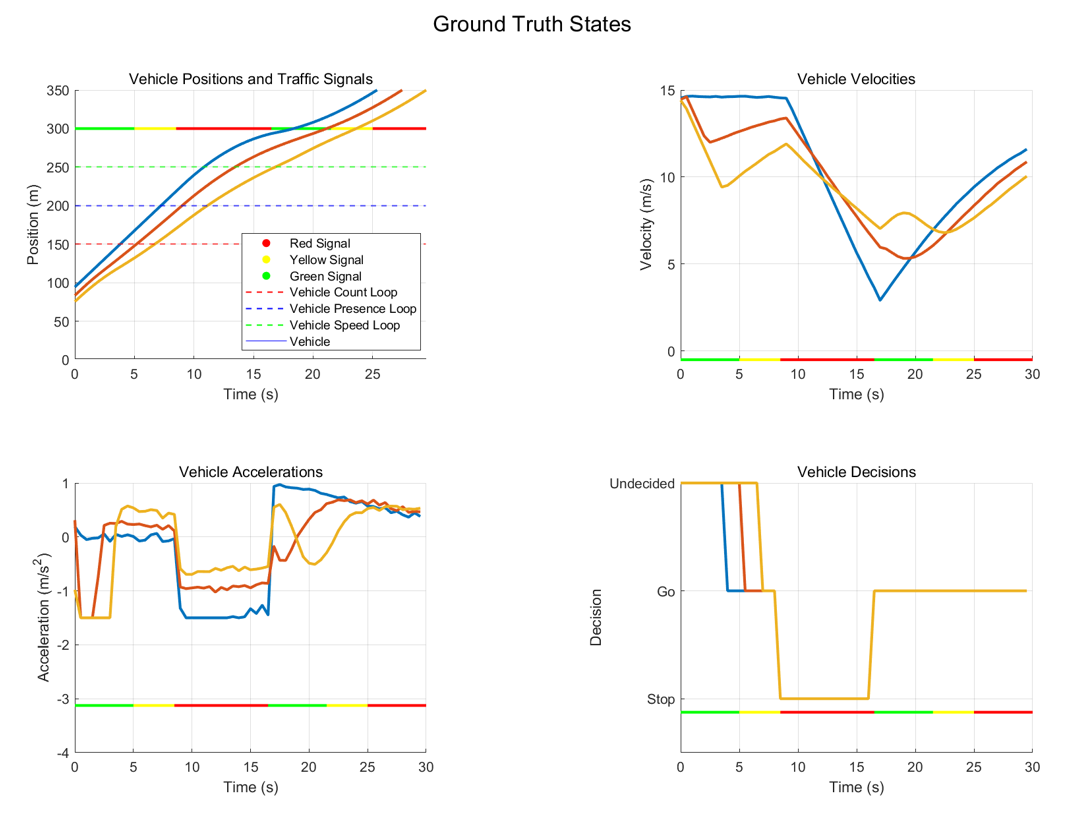
\includegraphics[width= 1\linewidth]{figures/groundtruth-3vehicles.png}
    \caption{Ground truth states, 3vehicles}
    \label{fig: groundtruth-3vehicles}
\end{figure}

In subplot 4, the blue line represents the leading vehicle, showing that it begins making a decision at 4 seconds. In subplot 1, around 4 seconds, the vehicle enters the decision zone and initiates its decision-making process. The parameter $D_h = 150\,\text{m}$ indicates that the vehicle starts making decisions when it approaches 150 meters from the stop line.

The traffic signal timing is as follows: green time is 5 seconds, yellow time is 3.5 seconds, and red time is 8 seconds, with the stop line located at 300 meters. In subplot 1, the vehicle count loop is positioned at 150 meters, the vehicle presence loop at 200 meters, and the vehicle speed loop at 250 meters. In this figure, the leading vehicle decides to stop at the end of the yellow phase and maintains this decision throughout the red phase.


\begin{figure}[H]
    \centering
    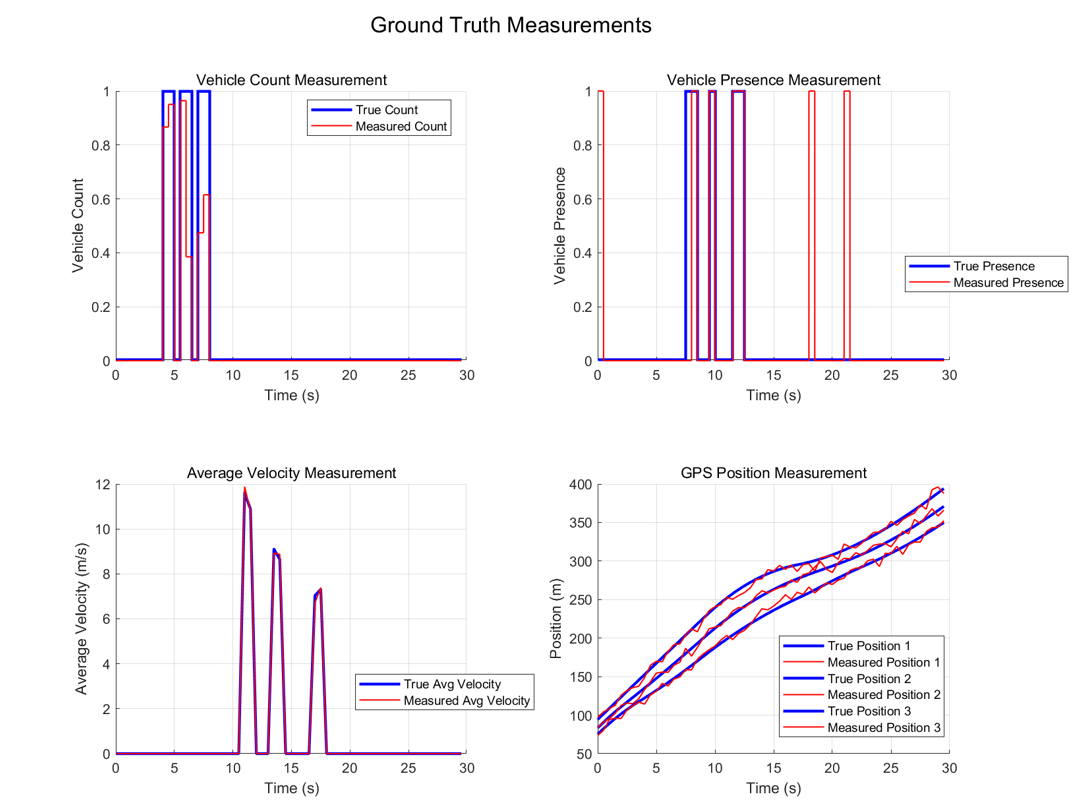
\includegraphics[width= 1\linewidth]{figures/groundtruth measurement.png}
    \caption{Ground truth measurements}
    \label{fig: Ground truth measurements}
\end{figure}

Subplot 1 displays the vehicle count loop, with the true counts occurring around 4, 5.25, and 7 seconds, which aligns with the ground truth states. The measured counts, represented by the red line, are noisy. Subplot 2 shows the vehicle presence loop, where the measured presence aligns with the accuracy parameter of 0.95. Subplot 4 presents the noisy position measurements obtained from GPS. These noisy measurements are intended to serve as inputs for the particle filter during the measurement-based correction step. However, since the particle filter process is not yet complete, these are the full set of simulation results from my work at this stage.

\begin{figure}[H]
    \centering
    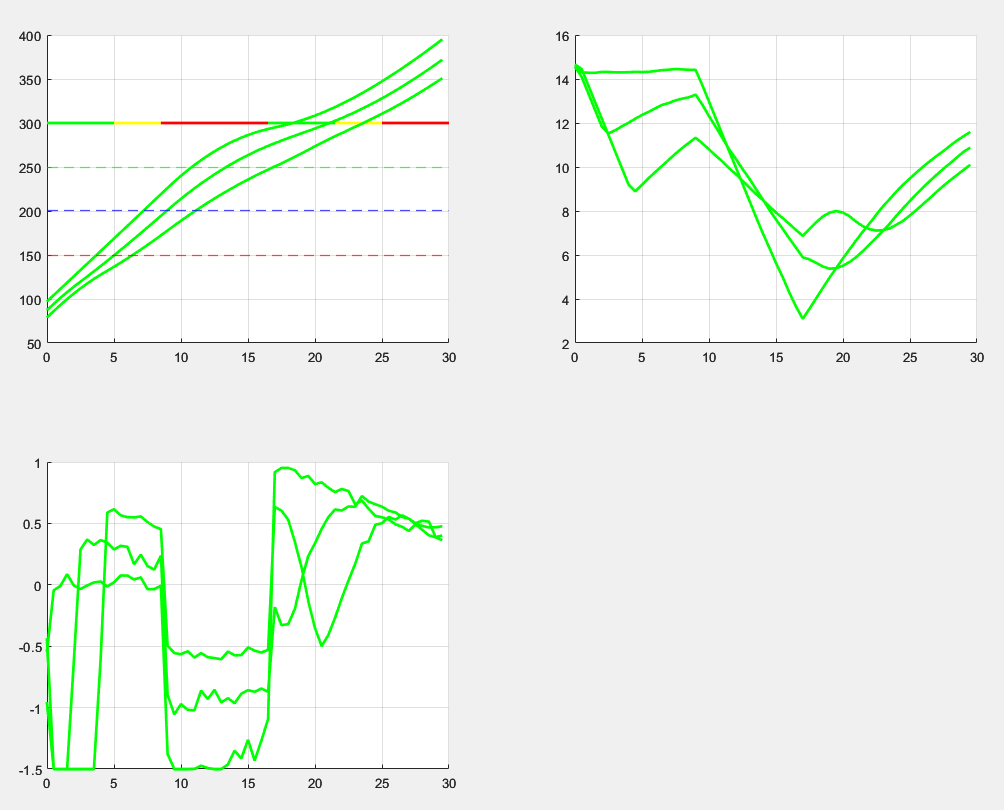
\includegraphics[width= 1\linewidth]{figures/particle filter.png}
    \caption{Unfinished particle filter}
    \label{fig: particle filter}
\end{figure}

The expected outcome is that the green line represents the ground truth states, with particles scattered around it. When the particle filter receives noisy measurements from the loops, particles closer to the ground truth are expected to have larger weights, shows a larger size, reflecting their higher likelihood of accuracy.

\subsection{Procedure}
The procedure will outline the steps for setting initial conditions, starting simulations, and collecting data.
\begin{itemize}
    \item \textbf{Initialization:} To ensure consistency within the particle filter process, the initialization for generating ground truth states, state-based prediction output, and measurement-based correction output follows the same procedure. The initialization step uses predefined bounds to generate initial states for position, velocity, acceleration, and decision for each particle, with each particle representing the states of all vehicles.
    \item \textbf{Simulation:} The simulation begins by generating traffic signal states through the state transition function module. The initial states are then passed to the simulation function to generate the ground truth states and corresponding measurements.
    \item \textbf{Main Process:} In the main script, the ground truth data is plotted, and the initial particles proceed with the state-based prediction. Once the ground truth measurements are received, the particle filter updates the weights, performs resampling, and ultimately produces the state estimations.
\end{itemize}

\subsubsection{Repetitions and Variations}
The parameter \textit{num\_iterations} is adjustable and depends on the traffic signal cycle time. To capture the decision-making process during the yellow phase, \textit{num\_iterations} must be at least longer than the duration of one complete traffic signal cycle.




\subsubsection{Invalidate results: generate state-based prediction output for single vehicle}

\begin{figure}[H]
    \centering
    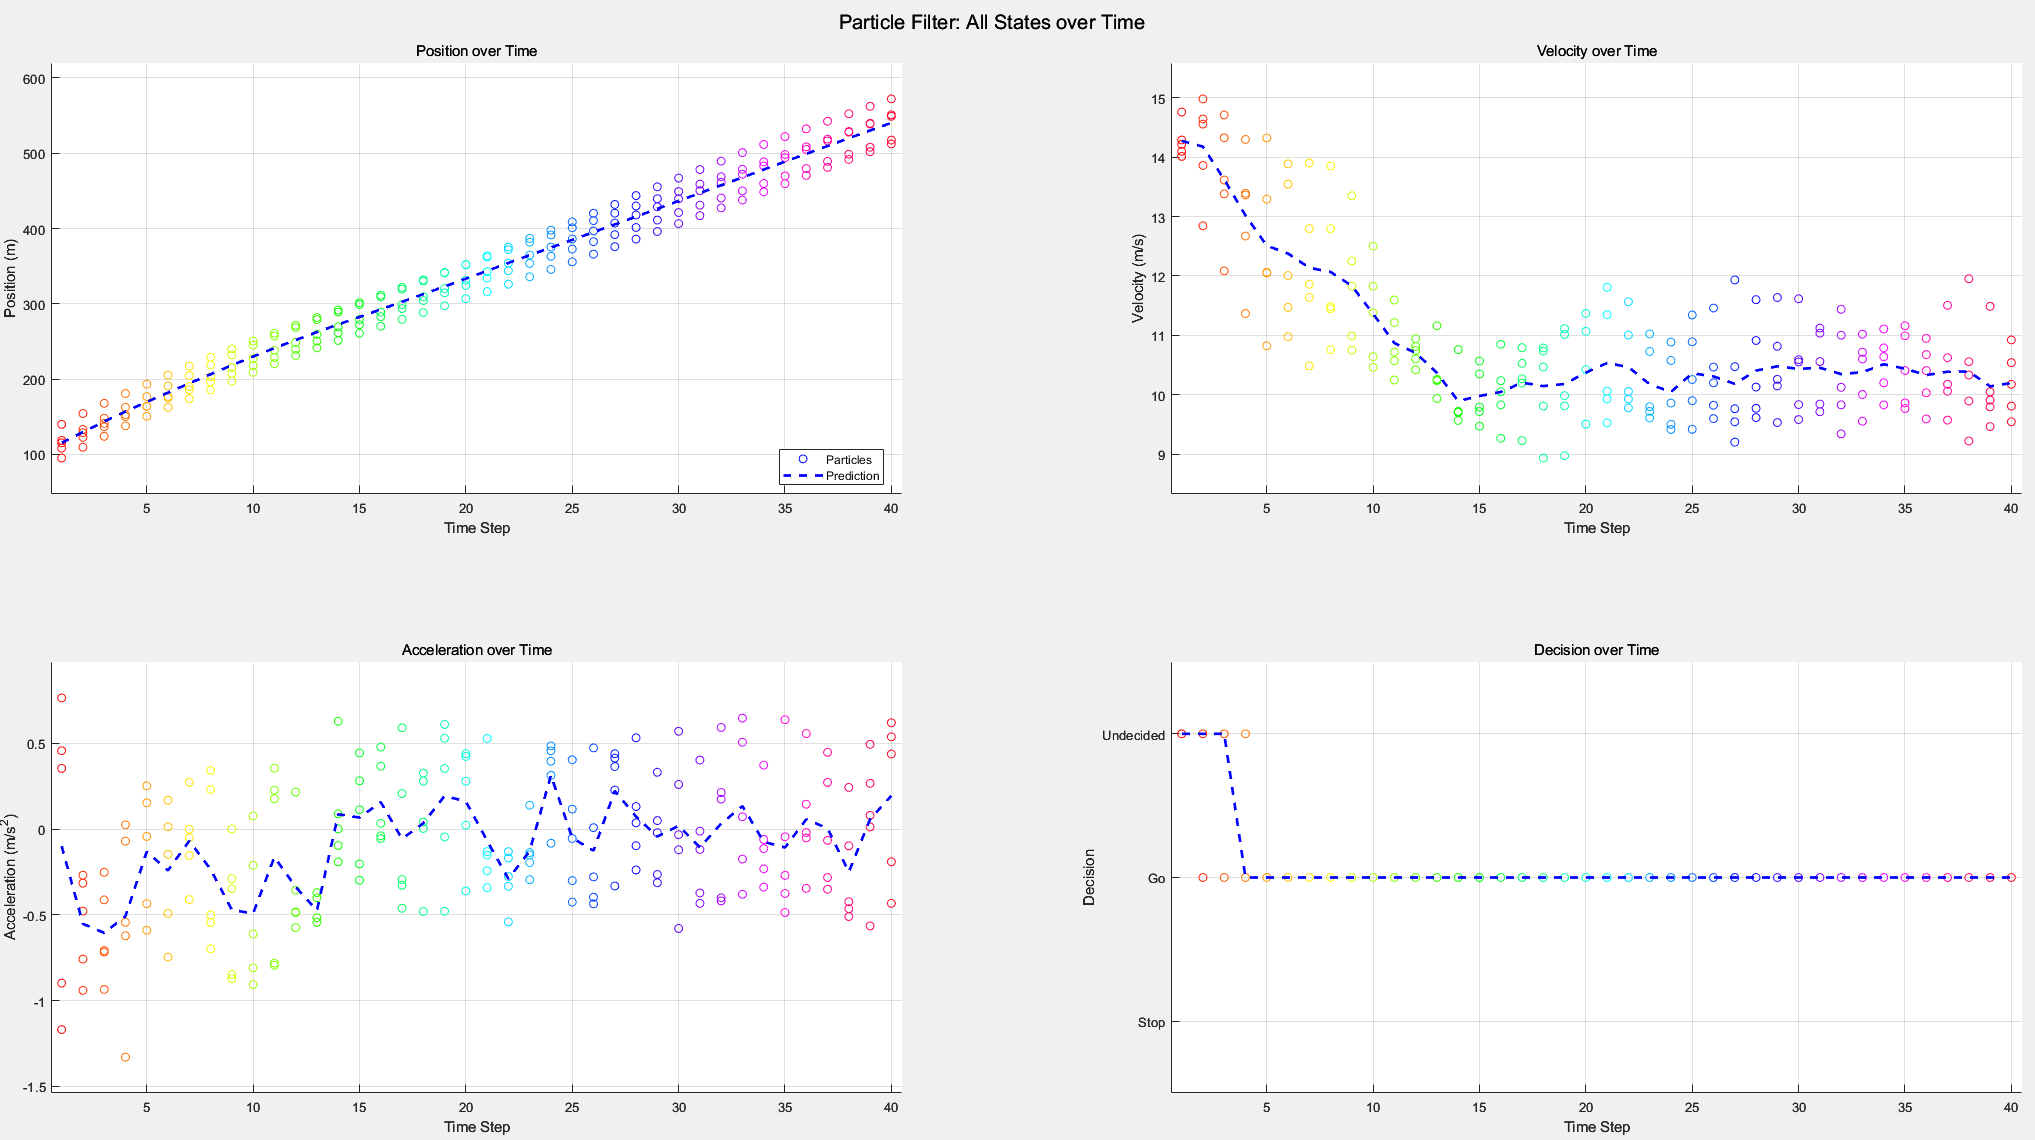
\includegraphics[width= 1\linewidth]{figures/Scenario 1.2.1-1, generate state-based prediction output for single vehicle.png}
    \caption{generate state-based prediction output for single vehicle, $N_\text{particles} = 5$}
    \label{fig: Scenario 1.2.1-1, generate state-based prediction output for single vehicle}
\end{figure}

\begin{figure}[H]
    \centering
    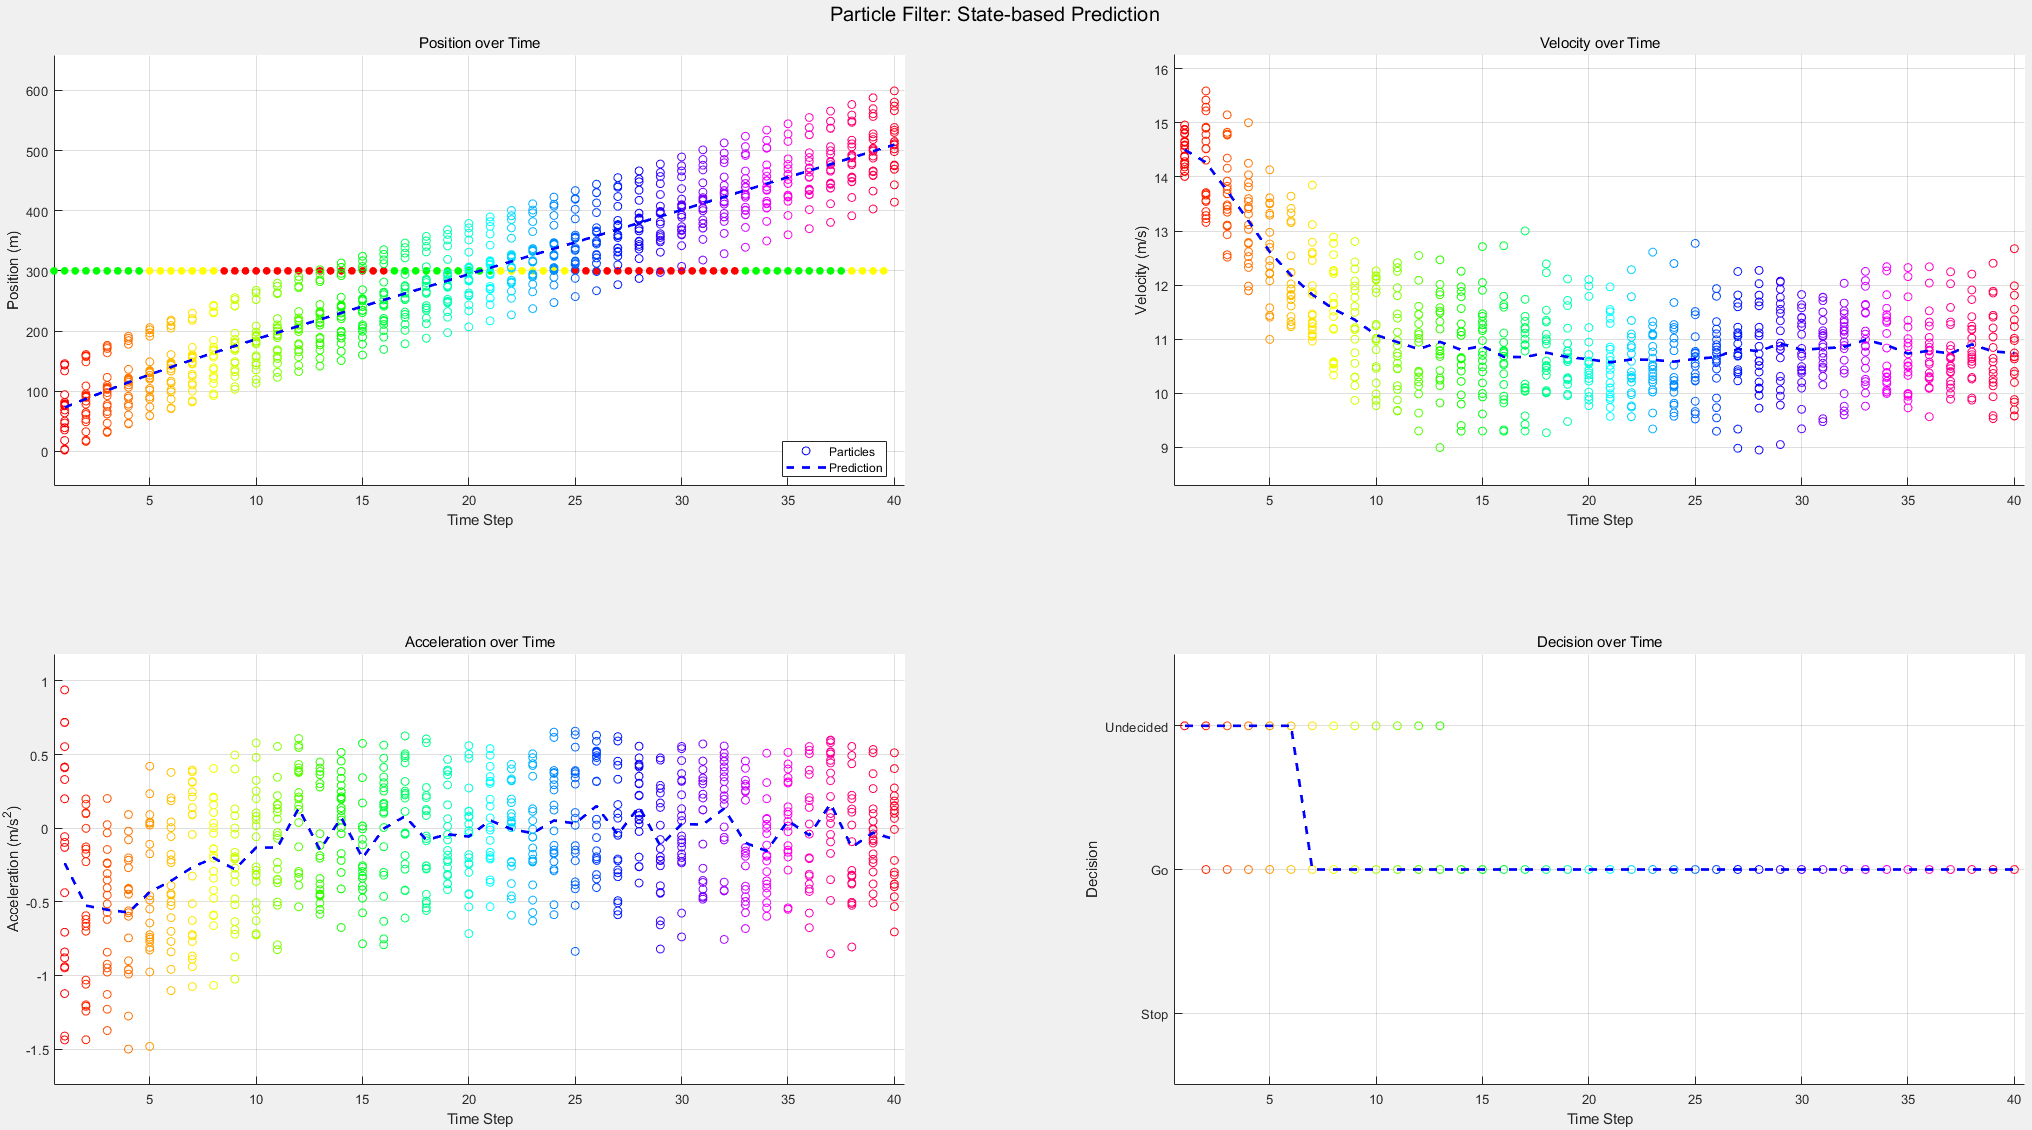
\includegraphics[width= 1\linewidth]{figures/Scenario 1.2.1-2, generate state-based prediction output for single vehicle.png}
    \caption{generate state-based prediction output for single vehicle, $N_\text{particles} = 20$}
    \label{fig: Scenario 1.2.1-2, generate state-based prediction output for single vehicle}
\end{figure}

\begin{figure}[H]
    \centering
    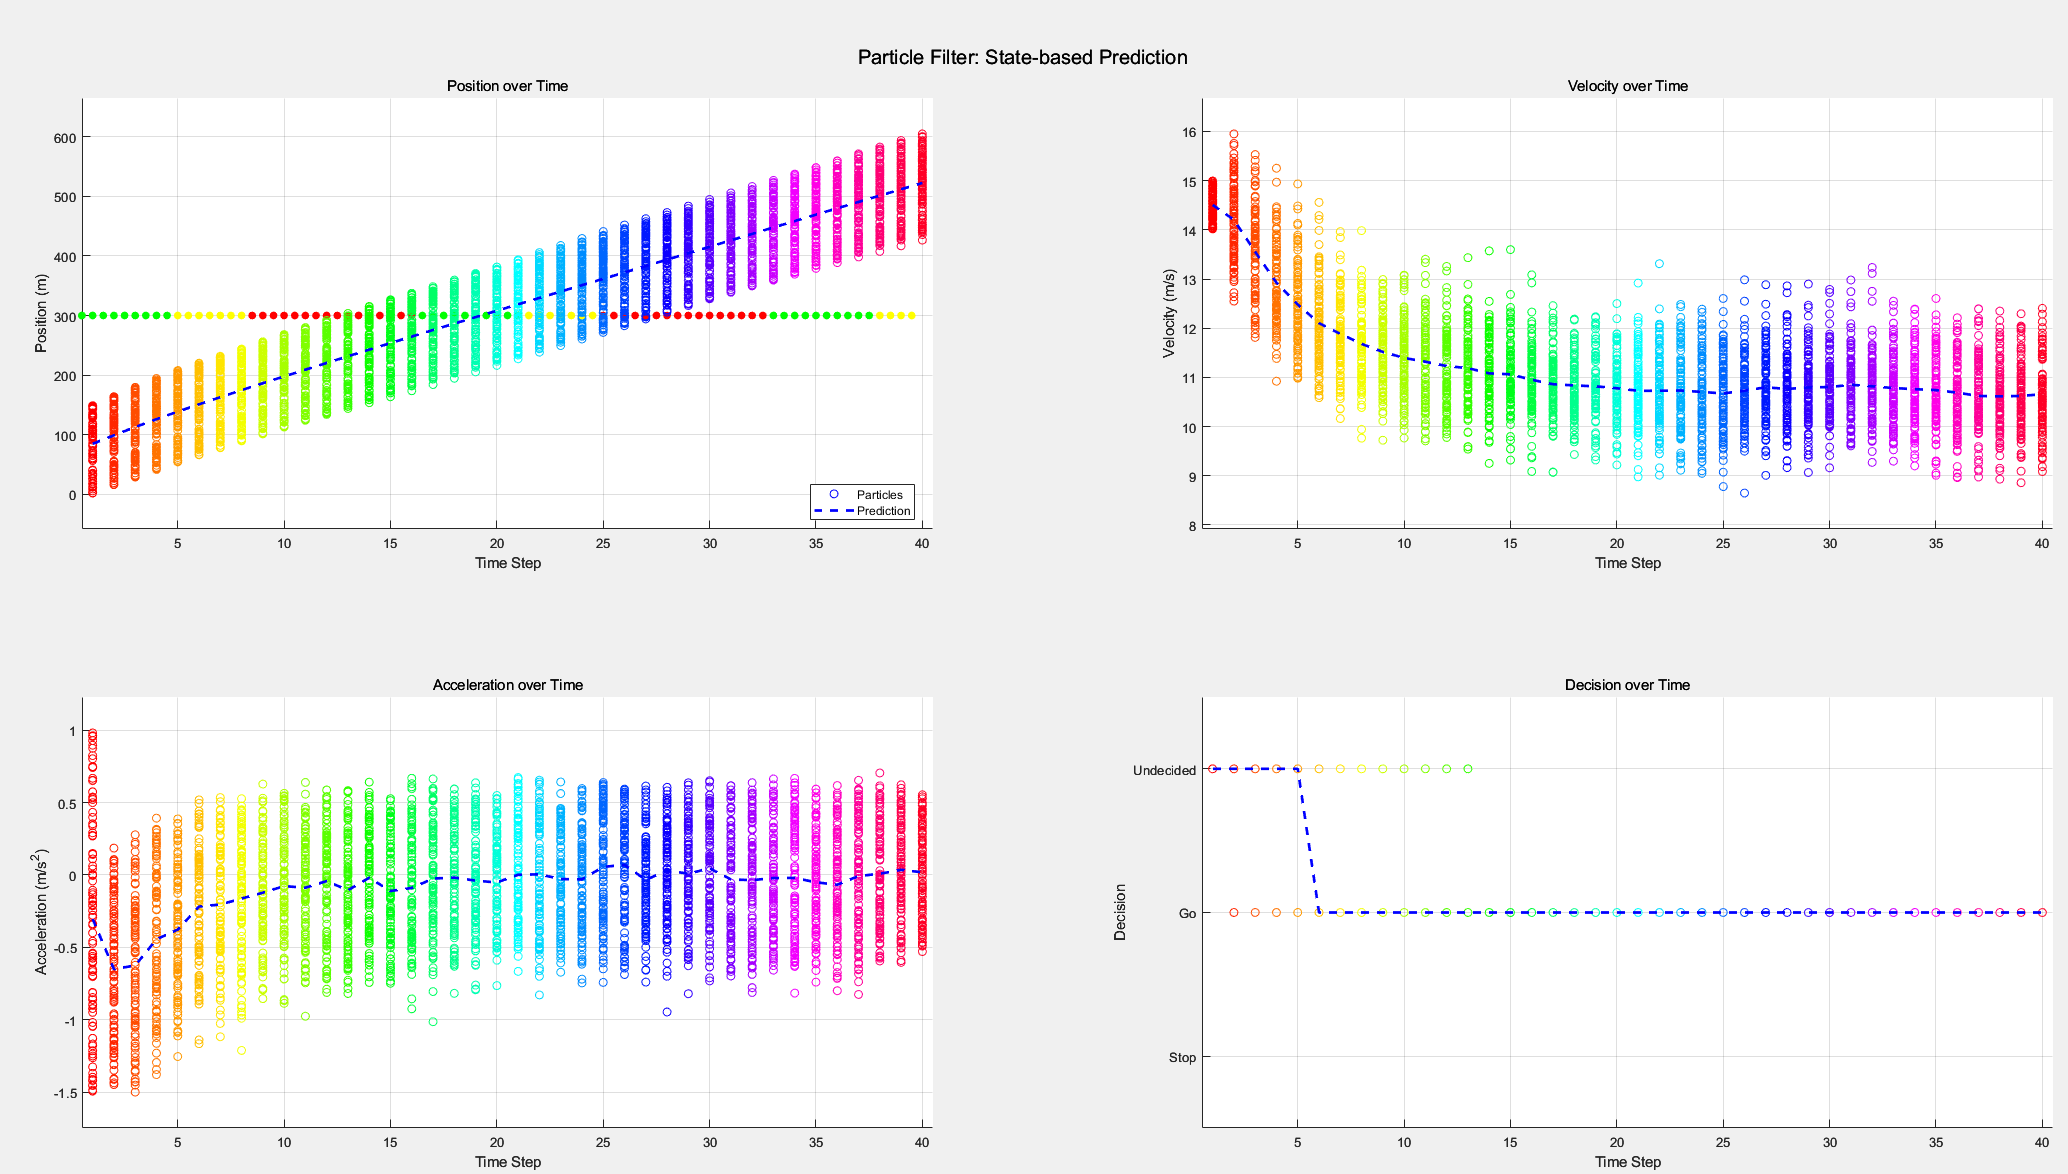
\includegraphics[width= 1\linewidth]{figures/Scenario 1.2.1-3, generate state-based prediction output for single vehicle.png}
    \caption{generate state-based prediction output for single vehicle, $N_\text{particles} = 100$}
    \label{fig: Scenario 1.2.1-3, generate state-based prediction output for single vehicle}
\end{figure}


\subsection{Future Work}
\begin{enumerate}
    \item \textbf{Sensitivity Analysis of $p_\text{stop}$:} \\
    Perform a sensitivity analysis on the decision parameters, particularly $p_\text{stop}$. This involves adjusting these parameters to assess their sensitivity and evaluate their impact on the performance of the PF-SIQE.
    
    \item \textbf{Sensitivity Analysis of Loop Detector Placement:} \\
    Investigate the sensitivity of PF-SIQE to the placement of loop detectors. This entails evaluating whether the performance of the estimator is influenced by the detector locations and, if so, determining the optimal positioning for maximum effectiveness.
    
    \item \textbf{Sensitivity to GPS Penetration Rate:} \\
    Assess the sensitivity of PF-SIQE to the penetration rate of GPS-equipped vehicles. The goal is to identify the minimum proportion of GPS-equipped vehicles required to ensure satisfactory performance of the queue estimator.
    
    \item \textbf{Evaluation of Particle Filter Parameters:} \\
    Explore the influence of particle filter parameters on the performance of PF-SIQE. This includes examining the effects of the number of particles, the threshold for the Effective Particle Number, and the impact of initial conditions. Key parameters to be tested include:
    \begin{itemize}
        \item Number of particles
        \item Threshold for Effective Particle Number
        \item Initial conditions
    \end{itemize}
\end{enumerate}







\section{Discussion}

\subsection{Interpretation of Results}
The primary objective of this thesis was to develop and apply the Particle Filter-Based Signalized Intersection Queue Estimator (PF-SIQE) to estimate vehicle queues at signalized intersections. Although the particle filter process was not fully visualized and validated, the validation of the traffic decision-making model was successfully completed. The ground truth states and the traffic signal state transitions were generated as planned, allowing for an initial evaluation of vehicle behavior during decision-making at intersections.

The key result is that the traffic decision-making model correctly captures vehicle responses in the dilemma zone based on the defined probability ($p_\text{stop}$). These results align with the expected decision patterns of vehicles in real-world scenarios, particularly in the transition from yellow to red lights. However, without the complete execution of the particle filter process, the accuracy of queue estimation and the filter's performance under noisy measurement conditions remain unverified.

\subsection{Validation}
The validation of the traffic decision-making model confirms its effectiveness in representing vehicle behavior in the dilemma zone. The model’s ability to handle stochastic decision-making offers promising potential for future research and application in traffic management systems. However, the particle filter’s validation, which was intended to assess how well the filter handles noisy measurements and updates particle weights, could not be completed due to the visualization challenges. Without this, the core performance of PF-SIQE in accurately estimating queue lengths cannot be fully evaluated at this stage.

\subsection{Limitations}
A significant limitation in this work is the incomplete execution of the particle filter process, which halted the full validation of the PF-SIQE model. As a result, key aspects such as parameter tuning for sensitivity analysis and performance validation under noisy conditions were not conducted. Additionally, due to the absence of real-world data, the model’s validation remains purely simulation-based, and further experiments are needed to verify its effectiveness in real-world applications. Future work should focus on resolving the particle filter visualization issues and extending the validation to include the entire filter process and a broader range of scenarios.

\section{Conclusion}

\subsection{Summary of Findings}
This thesis explored the development of the Particle Filter-Based Signalized Intersection Queue Estimator (PF-SIQE), focusing on real-time queue estimation at signalized intersections. While the particle filter process and its visualization remain incomplete, the traffic decision-making model was successfully validated, showing that it can accurately represent vehicle behavior in the dilemma zone. Ground truth states and measurements were generated as expected, but without completing the particle filter, further results, including accurate queue length estimations, could not be achieved.

\subsection{Implications}
The validation of the traffic decision-making model provides important insights into the potential for applying decision models in traffic management systems. However, the incomplete validation of the PF-SIQE model highlights the need for additional research to fully unlock the estimator's capabilities. Once fully developed and validated, PF-SIQE could significantly improve real-time traffic signal control and optimization by providing accurate queue length estimates, thus contributing to more efficient and adaptive intelligent transportation systems.

\subsection{Future Work}
Future research should focus on completing the particle filter visualization and validation. Key areas for improvement include optimizing the particle filter’s handling of noisy measurements, conducting parameter sensitivity tests, and validating the entire model with real-world traffic data. Expanding the model to incorporate lateral vehicle behavior, lane changes, and multi-lane intersections would also enhance its applicability in more complex urban traffic scenarios. Additionally, extending the research to investigate different particle filter resampling methods and noise models could further improve the accuracy and robustness of the queue estimation process.




 
\afterpage{\blankpage}
\chapter{Discussion, Conclusion, and Recommendation}
\label{chapter: Discussion, Conclusion, and Recommendation}


This chapter presents a comprehensive summary of the key findings from the research and how they align with the initial objectives. The chapter also revisits the main hypotheses and assumptions made during the study, examining their theoretical and practical implications. The discussion further evaluates the significance of the results within the broader context of intelligent transportation systems (ITS) and identifies any limitations encountered. Finally, the chapter offers recommendations for future research, highlighting areas where the PF-SIQE model can be further refined and extended. Through these insights, the conclusion encapsulates the core contributions of this research while outlining the potential path forward.

\section{Outcomes}

This thesis set out to develop a Particle Filter-based Signalized Intersection Queue Estimator (PF-SIQE) to estimate real-time queue lengths at signalized intersections, addressing several research objectives. Below is a summary of the key outcomes related to these objectives.

\begin{enumerate}
    \item \textbf{Developing a PF-SIQE architecture and algorithm framework:} \\
    The PF-SIQE architecture and algorithm framework were successfully developed, as detailed in Chapter \ref{chapter: Development of a Particle Filter-Based Signalized Intersection Queue Estimator (PF-SIQE)}. The architecture consists of three core modules: the particle filter module, the state transition function module, and the measurement function module. The modular design allows for flexibility and adaptability, making it possible to integrate various microscopic traffic flow models and observational data from different detection technologies. This meets the first research objective, as the framework is both scalable and adaptable to diverse traffic conditions and sensor inputs.

    \item \textbf{Studying detection technologies, their outputs, and corresponding noise distributions:} \\
    Chapter \ref{chapter:Literature Review} explored various detection technologies and their output measurements. The focus was on loop detectors and GPS data, with noise characteristics for these technologies discussed in Chapter \ref{chapter: Development of a Particle Filter-Based Signalized Intersection Queue Estimator (PF-SIQE)}. A key contribution of this thesis is the novel mathematical representation of noise characteristics for loop detectors, which enhances the adaptability of the PF-SIQE. While not all detection technologies were covered, the research successfully addressed this objective by examining the most relevant technologies for signalized intersection queue estimation.

    \item \textbf{Building a modular mathematical model and implementing it in simulation:} \\
    The modular mathematical model of the PF-SIQE was developed and implemented in a simulation environment, as described in Chapter \ref{chapter: Development of a Particle Filter-Based Signalized Intersection Queue Estimator (PF-SIQE)}. This model integrates the three core modules, utilizing state transition functions and measurements to estimate vehicle queues at intersections. The implementation verified the model's ability to function as designed, thus achieving the third objective.

    \item \textbf{Validation of the PF-SIQE:} \\
    Initial validation efforts focused on the traffic light decision-making model, demonstrating that vehicle behavior in simulations aligned with the decision strategies outlined in the model. Though additional sensitivity tests were initially planned, they were not fully completed due to time constraints. However, the validation results provide a solid foundation for the model's reliability. Further validation is recommended for future work to confirm the estimator’s performance under a broader range of conditions.
\end{enumerate}

By addressing these key objectives, this research has made significant progress in the development of a scalable, adaptable, and real-time signalized intersection queue estimator. While some areas, such as sensitivity analysis, will require future research, the outcomes presented here reflect a strong foundation for further development and practical application of the PF-SIQE.


\section{Discussions}


\subsection{Hypothesis}
This research was driven by the hypothesis that a particle filter-based algorithm can accurately estimate real-time queue lengths at signalized intersections, while offering flexibility and adaptability to different data sources. The validation of the traffic light decision-making model supported this hypothesis, demonstrating that vehicle behavior—such as the decision to stop or proceed—was consistent with the designed strategies. This provides a strong foundation for the application of particle filters in dynamic, real-time traffic scenarios. Furthermore, the modularity of the PF-SIQE framework enables it to handle various detection technologies and adapt to different traffic environments, enhancing its potential for practical implementation.

\subsection{Assumptions}
\begin{itemize}
    \item \textbf{Driver Decision Distance ($D_h = 150$ m):} \\
    It is assumed that when a vehicle is within 150 meters of the traffic signal, the driver begins making decisions to stop or proceed based on the signal status. This assumption is based on standard visibility requirements in ideal conditions. However, factors such as weather, road layout (e.g., curves, gradients), and obstacles can influence a driver's decision-making process. Relaxing this assumption would require dynamic modeling of visibility conditions and driver response times, which could alter the estimated queue lengths. In practice, adjusting the decision distance based on site-specific investigations would provide more accurate estimates for different intersections.

    \item \textbf{Vehicle Arrival and Departure:} \\
    This research assumes that the number of vehicles in the study area remains constant over time—when one vehicle exits, another immediately enters. While this simplifies the modeling process, it does not reflect real-world traffic dynamics, where vehicle arrivals and departures are more complex and stochastic. To model varying numbers of vehicles, changes would be needed in the state transition functions, where variable entry and exit rates could be introduced. The model would also need to account for factors such as vehicle platooning, traffic signal timing, and varying traffic demand across time periods.

    \item \textbf{GPS Data Labeling:} \\
    The model assumes that it is possible to identify which vehicle is associated with each GPS reading. In reality, GPS data may not always be labeled for individual vehicles, particularly in non-commercial settings. However, certain commercial fleets do share their real-time positions. Relaxing this assumption would require developing techniques to associate GPS signals with specific vehicles, such as vehicle re-identification algorithms or data fusion methods. Overlapping signals from nearby vehicles and GPS inaccuracies, particularly at low speeds, remain significant challenges to address in practical implementations.

    \item \textbf{Queue Definition:} \\
    The definition of a queue in this thesis is based on a velocity threshold: vehicles are considered to be in a queue if their velocity is below a certain threshold and they occupy a cumulative distance corresponding to the standard vehicle length. This assumption simplifies the process but has limitations. For instance, it does not account for different vehicle types, which may have varying lengths and behaviors. Additionally, determining the velocity threshold is a topic for further study, as this can significantly influence queue length estimation. A known drawback is that once a red light turns green, the queue may appear to suddenly disappear within a single time step, even though vehicles are still present in the intersection. This highlights the importance of integrating vehicle arrival and departure dynamics into future models.

    Moreover, the definition of a queue varies across the literature depending on the study's objective. For the purpose of studying signal cycle performance, defining the queue as vehicles with near standstill velocity may be most appropriate. However, other definitions could serve different purposes, such as analyzing traffic congestion or vehicle delays. As such, the choice of queue definition in this thesis is pragmatic and aligns with the objective of improving real-time traffic signal control.

    \item \textbf{Speed Loop Detector:} \\
    The algorithm used with the speed loop detector differentiates between whether a vehicle is passing through or not. However, the current model lacks consideration for situations where a vehicle is stationary on the detector. Accurately identifying when a vehicle is at a standstill on the detector is crucial for detecting and analyzing queues. This limitation needs to be addressed in future work to improve the accuracy of queue estimation and traffic flow analysis.

    \item \textbf{Comparison with Other Queue Estimators:} \\
    This research does not include a comparison with other queue estimators, such as the Extended Kalman Filter, for two main reasons: time constraints and uncertainty about the comparability of different approaches to handle noise. Kalman filters and their variants (such as the Unscented Kalman Filter, Ensemble Kalman Filter, and Adaptive Kalman Filter) approach noise and uncertainty differently than particle filters, which may make direct comparisons challenging. A comprehensive study of these variants would also require significant additional time. Therefore, such comparisons are considered potential future work.
\end{itemize}

\subsection{Theoretical Implications}
Theoretically, this research contributes to the growing body of knowledge on real-time, microscopic level traffic modeling and estimation using particle filters. The PF-SIQE framework pushes the boundaries of queue length estimation by offering a flexible, scalable architecture that can be applied across different detection technologies and traffic scenarios. This ability to adapt to diverse data sources, combined with high-resolution queue tracking, represents a significant improvement over traditional macroscopic models. Additionally, relaxing some of the assumptions mentioned earlier could lead to more realistic models, further enhancing the theoretical foundation for real-time traffic estimation.

These advancements address the immediate need for more granular traffic management solutions and open new pathways for future research in particle filter-based queue estimation algorithms. The exploration of more complex vehicle dynamics, such as varying arrival and departure rates, is a crucial area for extending the current model.

\subsection{Practical Implications}
From a practical perspective, the PF-SIQE model holds great potential for applications in intelligent transportation systems (ITS), such as Vehicle-to-Infrastructure (V2I) and Infrastructure-to-Vehicle (I2V) communications, adaptive traffic signals, and Green Light Optimal Speed Advisory (GLOSA) systems. However, several key assumptions—such as the reliance on simulated data for validation—highlight the gap between this research and real-world deployment.

Before the model can be effectively implemented in urban environments, it is necessary to validate it using real-world data. This validation would involve comparing the PF-SIQE’s estimations with actual traffic data collected from signalized intersections. One potential source of such data is phased array radar systems (refer to Prof. Hao Yue's lab in Beijing Jiaotong University), which can provide position, speed, and other detailed metrics for each vehicle at an intersection. Although these radar systems offer continuous monitoring, the data they produce may be imprecise and contain noise, necessitating extensive pre-processing before it can be used for validation purposes. Noise reduction and data cleaning will be critical steps in ensuring that the input data aligns with the assumptions of the PF-SIQE model.

In addition, real-world data collection from GPS-equipped vehicles, especially those within commercial fleets, would help validate the model's ability to estimate vehicle queues in diverse traffic conditions. While labeled GPS data may be available for certain vehicles, general traffic scenarios would require advanced vehicle identification techniques, such as data fusion from multiple sensors, to reliably track vehicles through an intersection.

Other key considerations include optimizing the placement of loop detectors and understanding the penetration rates of floating car sensors to ensure accurate data inputs for the model. Accurate real-time data on vehicle positions, speeds, and movements are essential for validating the particle filter’s state transition and measurement functions.

These refinements will help bridge the gap between the theoretical framework presented in this research and its practical deployment in real-world traffic management solutions.



\section{Recommendations for Future Work}

Several promising directions for future work arise from this research:

\subsection{State Transition Function Module}
    \begin{itemize}
        \item Integrate lateral microscopic models, such as lane change models, into the state transition function module to handle lateral vehicle movements. For instance, introducing $i_{k+1}^\text{lane} = g(x_k, i_k^{\text{lane}}, \text{lane change external factors}, n_k^\text{lateral})$ to describe lane changes and lateral motion more accurately.
        \item Simulate multiple lanes and turning motions at more complex intersections to extend the applicability of the model beyond simple intersections. These simulations would test the impact of lane changes, turning motions, and lane-specific configurations on queue estimation and traffic flow.
        \item The road layout will be expanded in the estimator to include the following characteristics:
        \begin{itemize}
            \item Number of lanes,
            \item Type of lanes (e.g., through lanes, dedicated turning lanes, bus lanes),
            \item Direction of traffic flows.
        \end{itemize}
    \end{itemize}

\subsection{Measurement Function Module}
    \begin{itemize}
        \item Incorporate data from a wider range of detection technologies, and explore different combinations of these data sources (e.g., loop detectors, GPS, phased array radar) to assess their impact on the estimator’s accuracy. 
        \item Study how the placement of loop detectors and radar affects estimation results, and optimize detector configurations for various intersection types. Phased array radar data, despite containing noise and inaccuracies, could be processed to provide detailed information on vehicle positions and speeds.
        \item Analyze how varying levels of floating sensor penetration (e.g., GPS-equipped vehicles) influence the estimator’s performance, particularly in real-world scenarios.
    \end{itemize}

\subsection{Particle Filter Module}
    \begin{itemize}
        \item Investigate how the number of particles affects estimation accuracy and computational efficiency, and test different resampling methods (e.g., systematic resampling, stratified resampling) to improve performance. 
        \item Explore alternative paradigms for particle representation, such as assigning multiple particles to individual vehicles or employing a hierarchical filtering approach where each vehicle is tracked using its own particle filter, allowing for collaborative filtering between vehicles.
    \end{itemize}

\subsection{Queue Estimation}
    Queue estimation, a key feature of the PF-SIQE, can be enhanced by refining the velocity threshold method used for determining the number of stationary vehicles. In this thesis, the queue is estimated by counting vehicles with speeds below a threshold. Future work should focus on:
    \begin{itemize}
        \item Developing more dynamic thresholding techniques that account for acceleration and deceleration during signal transitions, avoiding abrupt changes in queue estimates when vehicles start moving simultaneously at green lights.
        \item Extending the state space representation to handle varying arrival and departure rates, which would model real-world scenarios more effectively. This could involve modifying the state transition equations to include time-varying vehicle entries and exits.
    \end{itemize}

\subsection{Simulation Sensitivity Analysis}
\begin{itemize}
    \item Conduct sensitivity analyses on factors such as acceleration noise, loop detector placement, GPS noise distribution, and floating sensor penetration to better understand their influence on the estimator’s performance. These analyses will provide insights into how different detection technologies and environmental conditions affect the PF-SIQE’s accuracy.
\end{itemize}

\subsection{Real-World Implementation}
\begin{itemize}
    \item Real-world testing is a crucial next step to ensure the PF-SIQE model’s practical applicability. This testing should be conducted using actual traffic data collected from signalized intersections. Phased array radar systems, like those available at Prof. Hao Yue's lab in Beijing Jiaotong University, or GPS data from vehicles, could provide valuable insights into vehicle dynamics at intersections. These data sources, while continuous, will require careful pre-processing—such as noise filtering and data smoothing—to align with the assumptions of the PF-SIQE.
    
    \item In addition to validating the model's performance with real-world data, these tests should focus on assessing the PF-SIQE’s robustness across varying intersection types, lane configurations, and traffic conditions. This includes examining different traffic flow patterns, vehicle densities, and detection technologies. Such testing will not only fine-tune the model for practical use but also highlight areas for further refinement or adaptation of the algorithm.
\end{itemize}















\afterpage{\blankpage}


%% Prevent urls running into margins in bibliography
\setcounter{biburlnumpenalty}{7000}
\setcounter{biburllcpenalty}{7000}
\setcounter{biburlucpenalty}{7000}

%% Add bibliography

\printbibliography[heading=bibintoc,title=References]

%% ----------------------------------------------------------------------
%%    Appendix (Letters for chapters)
%% ----------------------------------------------------------------------

\appendix

\chapter{Summary of the list of Criteria}
\label{appendix: Summary of the list of Criteria}

This table provides a summary of key criteria that can be used to evaluate the performance of the PF-SIQE model and other estimation algorithms. These criteria are relevant for assessing the accuracy, robustness, and efficiency of the model in various traffic conditions, making them crucial for understanding the model's practical implications and identifying areas for future improvement.
\section{Selecion of the Appropriate Evaluation Criteria}\label{Selecion of the Appropriate Evaluation Criteria}
A performance evaluation framework requires the careful selection and definition of criteria to assess the PF-SIQE's performance. Appendix \ref{appendix: Summary of the list of Criteria} presents various criteria used in the evaluation of model performance. The selection of appropriate evaluation criteria is crucial and must align with the specific performance requirements. It is important to consider how the characteristics and advantages of each criterion match these requirements and why the disadvantages may be negligible in this context.

The primary requirement for the PF-SIQE is to accurately estimate queue lengths at signalized intersections while effectively handling noisy measurements. Mean Absolute Error (MAE) offers a clear measure of the average magnitude of errors in estimations, which is directly pertinent to evaluating the accuracy of queue length estimates. Unlike Mean Squared Error (MSE), which can be disproportionately affected by large errors, MAE treats all errors equally. This is particularly important in traffic management systems where occasional large errors, due to sudden stops, accelerations, or atypical behavior, should not unduly influence performance evaluation. MAE is well-suited for such applications, as maintaining consistent accuracy is more critical than minimizing the effect of infrequent large deviations. Hence, this thesis selects MAE as the primary and overall criterion.




High particle diversity is crucial for the PF-SIQE, as it enhances robustness and adaptability, allowing the filter to recover from incorrect estimations. This capability is essential in dynamic vehicular traffic systems, where states can change unpredictably. Therefore, studying particle diversity as an additional criterion is necessary. Particle diversity can be evaluated by calculating the effective number of particles, which is previously defined in Equation \ref{eq: effective number of particles}: $\widehat{N^{eff}} = \frac{1}{\sum_{j=1}^N ({w}_k^{j})^2}$. Where, \(\widehat{N^{eff}}\) represents the effective number of particles, and \({w}_k^{j}\) denotes the weight of the \(j\)-th particle at time step \(k\). When the effective number of particles falls below a certain threshold, resampling should be performed to maintain diversity and ensure accurate state representation.

By selecting MAE as the primary criterion and Particle Diversity as a supplementary criterion, the evaluation framework aligns well with the specific performance requirements of the PF-SIQE. MAE ensures precise and robust queue length estimations, while Particle Diversity ensures the filter's adaptability and robustness to changing traffic conditions. These criteria together provide a comprehensive evaluation of the PF-SIQE's performance in real-world traffic management scenarios.
\newgeometry{landscape, left=1cm, right=1cm, top=1.5cm, bottom=1.5cm}
\begin{landscape}
\begin{table}
\centering
\footnotesize 
\caption{Summary of the list of Criteria}
\label{Summary of the list of Criteria}
% 为各列分配不同的相对宽度
\begin{tabularx}{\linewidth}{@{} l 
>{\hsize=1.2\hsize}X  
>{\hsize=.8\hsize}X  
>{\hsize=.9\hsize}X  
>{\hsize=.9\hsize}X 
>{\hsize=1.2\hsize}X 
@{}} 
\toprule
\textbf{Criterion} & \textbf{Definition and Equation} & \textbf{Characteristics} & \textbf{Advantages} & \textbf{Disadvantages} & \textbf{Applicable Scene} \\ 
\midrule
\textbf{Mean Squared Error} & The average of the squares of the differences between the estimated and actual values. \newline
\( \text{MSE} = \frac{1}{n} \sum_{i=1}^{n} (y_i - \hat{y}_i)^2 \) & Emphasizes larger errors due to squaring. & Sensitive to large errors, making it useful for applications where such errors are particularly undesirable. & Can be overly influenced by outliers. & Useful in tracking and navigation applications where minimizing large deviations is crucial. \\ 
\midrule
\textbf{Mean Absolute Error} & The average of the absolute differences between the estimated and actual values. \newline
\( \text{MAE} = \frac{1}{n} \sum_{i=1}^{n} |y_i - \hat{y}_i| \) & Provides a direct measure of error magnitude without emphasizing larger errors. & Less sensitive to outliers than MSE. & May not adequately penalize larger errors. & Effective in economic forecasting where outliers can be common but large errors are not disproportionately penalized. \\ 
\midrule
\textbf{Root Mean Squared Error} & The square root of MSE. \newline
\( \text{RMSE} = \sqrt{\text{MSE}} \) & Balances between the magnitude of errors and their frequency. & More interpretable in terms of error magnitude than MSE. & Still sensitive to outliers. & Useful in energy demand forecasting, where error magnitude in predictions can have significant implications. \\ 
\midrule
\textbf{Maximum Absolute Error} & The largest absolute difference between the estimated and actual values. \newline
\( \text{Max Error} = \max(|y_i - \hat{y}_i|) \) & Indicates the worst-case error. & Useful for understanding the maximum possible error. & Does not provide information about typical errors. & Important in safety-critical applications, such as autonomous driving, where the worst-case scenario needs to be minimized. \\ 
\midrule
\textbf{Coverage Probability} & The probability that the true value falls within a specified confidence interval around the estimated value. & Measures the reliability of the confidence intervals. & Directly relates to the confidence one can have in the predictions. & Can be difficult to compute for non-linear models. & Valuable in statistical weather forecasting where providing reliable confidence intervals is as important as the predictions themselves. \\ 
\midrule
\textbf{Particle Diversity} & A measure of how spread out or varied the particles are in a particle filter. High diversity means the particles cover a wide range of the state space. & Indicates the ability of a particle filter to explore and represent the state space effectively. & Ensures that the filter can adapt to changes in the system dynamics and can recover from incorrect estimations. & Maintaining high diversity can be challenging, especially after resampling steps, which might lead to particle depletion. & Crucial in dynamic environments where the system's state can change unpredictably, such as in robotics navigation and tracking moving objects. \\ 
\midrule
\textbf{Cramer-Rao Lower Bound} & A theoretical lower bound on the variance of unbiased estimators. It provides a measure of the best possible accuracy that any unbiased estimator can achieve for a given parameter. %\newline
\( \text{Var}(\hat{\theta}) \geq \frac{1}{I(\theta)} \) & Serves as a benchmark to evaluate the efficiency of estimators. An estimator is considered efficient if it reaches the CRLB. & Offers a way to understand the inherent limitations in estimating a parameter and to assess the performance of estimators. & Applicable only to unbiased estimators and requires knowledge of the true parameter values, which may not always be available or clearly defined. & Useful in signal processing and communications, where it is important to evaluate the theoretical limits of system performance. \\ 
\bottomrule
\end{tabularx}
\end{table}
\end{landscape}
\restoregeometry






% performance criteria
%\chapter{source code}
%\label{chapter:title}
\emph{Adding source code to your report/thesis is supported with the package {\normalfont\texttt{listings}}. An example can be found below. Files can be added using {\normalfont\texttt{\textbackslash lstinputlisting[language=<language>]\{<filename>\}}}.}

\begin{lstlisting}[language=Python]
"""
ISA Calculator: import the function, specify the height and it will return a
list in the following format: [Temperature,Density,Pressure,Speed of Sound].
Note that there is no check to see if the maximum altitude is reached.
"""

import math
g0 = 9.80665
R = 287.0
layer1 = [0, 288.15, 101325.0]
alt = [0,11000,20000,32000,47000,51000,71000,86000]
a = [-.0065,0,.0010,.0028,0,-.0028,-.0020]

def atmosphere(h):
    for i in range(0,len(alt)-1):
        if h >= alt[i]:
            layer0 = layer1[:]
            layer1[0] = min(h,alt[i+1])
            if a[i] != 0:
                layer1[1] = layer0[1] + a[i]*(layer1[0]-layer0[0])
                layer1[2] = layer0[2] * (layer1[1]/layer0[1])**(-g0/(a[i]*R))
            else:
                layer1[2] = layer0[2]*math.exp((-g0/(R*layer1[1]))*(layer1[0]-layer0[0]))
    return [layer1[1],layer1[2]/(R*layer1[1]),layer1[2],math.sqrt(1.4*R*layer1[1])]
\end{lstlisting}






\emph{If a task division is required, a simple template can be found below for convenience. Feel free to use, adapt or completely remove.}

\begin{table}[htb]
    \setlength\extrarowheight{4pt}
    \centering
    \caption{Distribution of the workload}
    \label{tab:taskdivision}
    \begin{tabularx}{\textwidth}{lXX}
        \toprule
        & Task & Student Name(s) \\
        \midrule
        & Summary & \\
        Chapter 1 & Introduction &  \\
        Chapter 2 &  & \\
        Chapter 3 &  & \\
        Chapter * &  & \\
        Chapter * & Conclusion &  \\
        \midrule
        & Editors & \\
        & CAD and Figures & \\
        & Document Design and Layout & \\
        \bottomrule
    \end{tabularx}
\end{table}
% task division
%\input{appendix/appendix-c} % Create file to add

\end{document}
